\chapter{Cordillera}\label{dept:Cordillera}
\mapaparaguai{3}{Cordillera}
\vfill\clearpage
\clearpage
\subsection*{Análise Temática por Distrito}
\addcontentsline{toc}{subsection}{Análise Temática por Distrito}

Os mapas a seguir mostram, para cada distrito de Cordillera, o GSS final (pontuação geral), o risco social (criminalidade e instabilidade) e o potencial de autossuficiência (solo, água e energia). Cada valor é o calculado na metodologia GSS deste guia.

\begin{figure}[htbp]
\centering
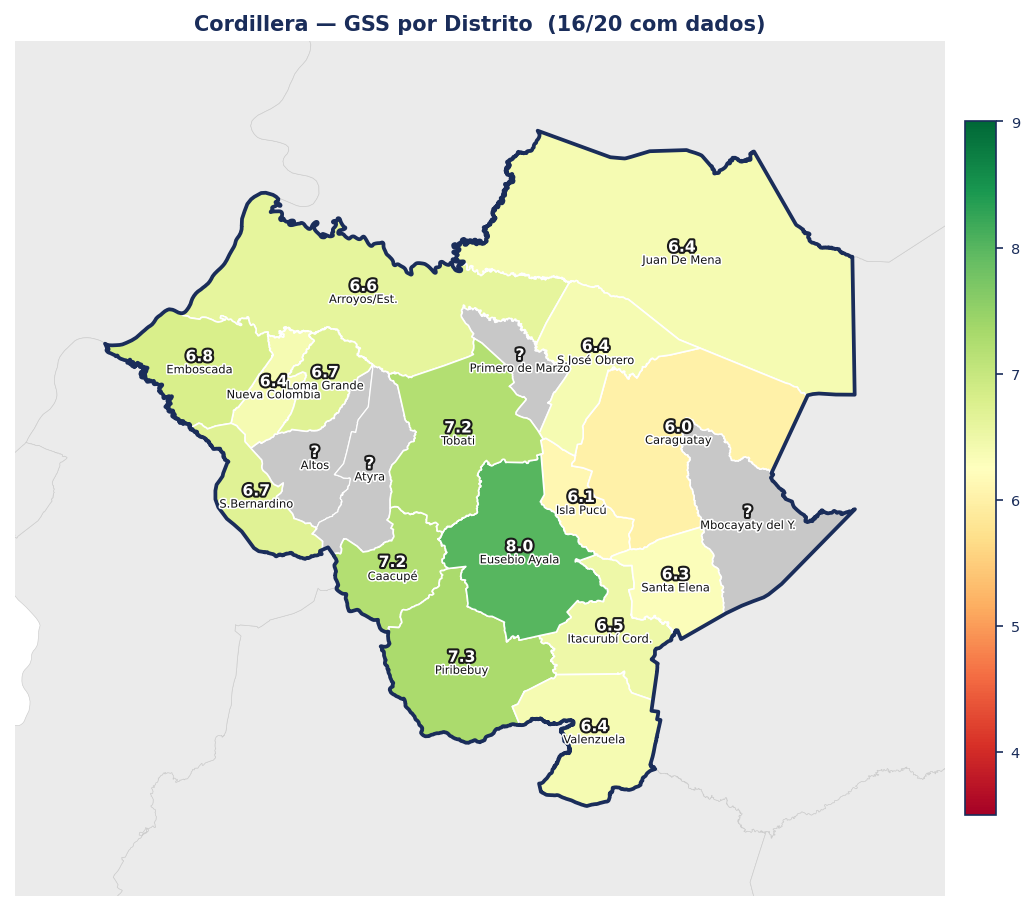
\includegraphics[width=\textwidth, height=0.55\textheight, keepaspectratio]{mapas/mapas_tematicos_dept_03_gss.png}
\caption{GSS (Global Safety Score) por distrito de Cordillera. Verde = alta viabilidade · Vermelho = baixa viabilidade.}
\label{fig:gss-03}
\end{figure}

\vspace{0.5em}

\begin{figure}[htbp]
\centering
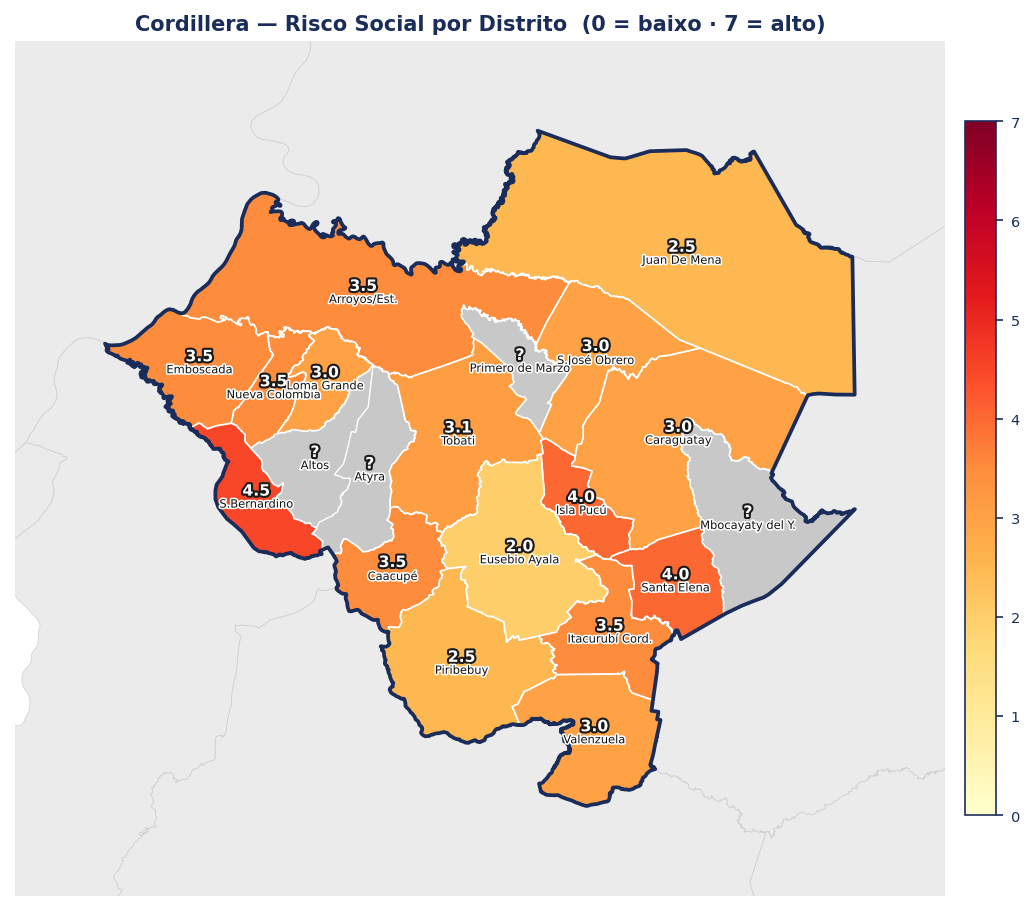
\includegraphics[width=\textwidth, height=0.55\textheight, keepaspectratio]{mapas/mapas_tematicos_dept_03_risco.png}
\caption{Risco social por distrito de Cordillera. Amarelo = baixo risco · Vermelho = alto risco.}
\label{fig:risco-03}
\end{figure}

\clearpage

\begin{figure}[htbp]
\centering
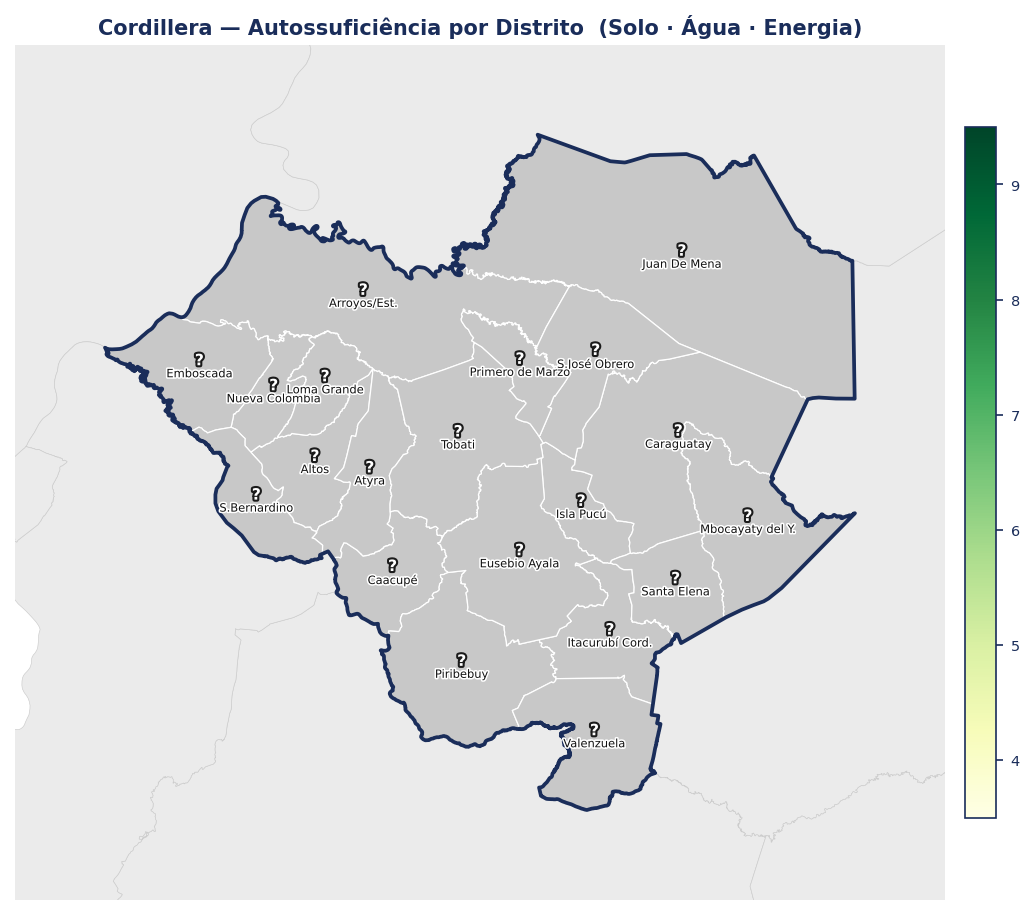
\includegraphics[width=\textwidth, height=0.55\textheight, keepaspectratio]{mapas/mapas_tematicos_dept_03_autosuf.png}
\caption{Autossuficiência por distrito de Cordillera: solo, recursos hídricos e potencial energético. Branco = baixo · Verde escuro = alto.}
\label{fig:autosuf-03}
\end{figure}

\clearpage

\section{Cordillera}

e uma malha territorial de transição entre a área metropolitana e o
interior produtivo.

\subsection{Ficha climática de Caacupe (capital
departamental)}

\textbf{Irradiância solar global --- (kWh/\allowbreak m²/\allowbreak dia):}


\begin{center}
\resizebox{\linewidth}{!}{%
{\renewcommand{\arraystretch}{1.2}%
\begin{tabular}{@{}c|c|c|c|c|c|c|c|c|c|c|c@{}}
\toprule
Jan & Fev & Mar & Abr & Mai & Jun & Jul & Ago & Set & Out & Nov & Dez \\
\midrule
6.76 & 6.20 & 5.42 & 4.44 & 3.36 & 2.83 & 3.21 & 3.93 & 4.61 & 5.49 &
6.42 & 6.78 \\
\bottomrule
\end{tabular}}%
}
\end{center}


Média anual: 4.95 kWh/\allowbreak m²/\allowbreak dia. Inclinação recomendada: 25° Norte (anual);
35° inverno; 15° verão.

\textbf{Precipitação --- (mm/\allowbreak mês):}


\begin{center}
\resizebox{\linewidth}{!}{%
{\renewcommand{\arraystretch}{1.2}%
\begin{tabular}{@{}c|c|c|c|c|c|c|c|c|c|c|c@{}}
\toprule
Jan & Fev & Mar & Abr & Mai & Jun & Jul & Ago & Set & Out & Nov & Dez \\
\midrule
127 & 140 & 133 & 148 & 152 & 78 & 66 & 41 & 77 & 171 & 193 & 175 \\
\bottomrule
\end{tabular}}%
}
\end{center}


Média anual: \textasciitilde1.500 mm/\allowbreak ano. Estação chuvosa Out-Mai; seca
Jun-Set.
\clearpage
\subsection*{Dados Departamentais}

\subsection*{Segurança Pública}

\begin{tabularx}{\linewidth}{lX}
\toprule
Indicador & Valor \\
\midrule
Taxa de homicídios (por 100k hab) & 3,5 (2022, fonte INE/Prosegur) \\
Crimes registrados (total/ano) & --- dados não desagregados publicamente \\
Número de comisarías & ~18 (estimativa departamental) \\
Índice segurança relativo & alto \\
\bottomrule
\end{tabularx}

Cordillera é um dos departamentos mais seguros do Paraguai. A taxa de homicídios de \textbf{3,5 por 100 mil habitantes} (2022) está significativamente abaixo da média nacional de 5,3 (2023) e muito abaixo dos departamentos fronteiriços problemáticos. O Ministerio Público registra que Cordillera responde por apenas \textbf{2\% das causas de homicídio doloso} do país --- proporção baixa considerando que é um departamento populoso próximo à capital.

O departamento não possui fronteira internacional e está geograficamente isolado de rotas principais de narcotráfico. Sua proximidade com Asunción (a capital está a menos de 80 km de Caacupé) facilita o acesso a serviços de segurança da capital. O turismo religioso em Caacupé (maior santuário mariano do Paraguai) gera movimentação econômica e maior presença policial em datas festivas.

A criminalidade predominante é patrimonial (furtos e roubos), especialmente em áreas com maior fluxo turístico. Violência com motivação de crimen organizado é rara no departamento.

\subsection*{IDH e Desenvolvimento Humano}

\begin{tabularx}{\linewidth}{lX}
\toprule
Indicador & Valor \\
\midrule
IDH & 0,718 \\
Classificação IDH & alto \\
Ranking nacional (1=melhor) & 6/18 \\
Esperança de vida & 73,5 anos \\
Anos de escolaridade média & 8,6 anos \\
RNB per capita (USD PPA) & 9.200 \\
\bottomrule
\end{tabularx}

> Nota: IDH estimado com base no relatório PNUD 2020 e dados subnacionais da Global Data Lab. Cordillera se beneficia da proximidade com Asunción e Central, apresentando IDH acima da média nacional. Estimativa com base nos dados publicados para a Região Central/Oriental paraguaia.

\begin{tabularx}{\linewidth}{lX}
\toprule
Indicador & Valor \\
\midrule
Taxa de pobreza total (\%) & 23,9\% \\
Taxa de pobreza extrema (\%) & 5,2\% \\
Índice de Gini & 0,440 \\
\bottomrule
\end{tabularx}

> Fonte: INE --- EPHC 2023 e Pobreza Multidimensional 2023 (IPM Cordillera: 20,22\%). Nota: houve aumento da pobreza em Cordillera entre 2022 e 2023 segundo relatório Última Hora.

\begin{tabularx}{\linewidth}{lX}
\toprule
Indicador & Valor \\
\midrule
Acesso a água potável (\%) & 82,4\% \\
Acesso a saneamento (\%) & 84,7\% \\
\bottomrule
\end{tabularx}

> Estimativa baseada no Censo 2022 e perfil semiurbano do departamento. Cordillera combina municípios turísticos (São Bernardino) com zonas rurais, resultando em cobertura heterogênea.

Cordillera é um departamento estrategicamente localizado entre Asunción e o interior do Paraguai, com IDH de 0,718 (alto). A proximidade com a capital (a apenas 50-70 km) permite acesso a serviços de saúde e educação de qualidade, enquanto o custo de vida é menor. Caacupé, capital departamental e sede do maior santuário mariano do Paraguai, oferece infraestrutura razoável. São Bernardino no lago Ypacaraí é área turística valorizada, com imóveis disputados e qualidade de vida elevada. Para brasileiros, Cordillera representa boa relação custo-benefício: mora-se com mais espaço e conforto do que em Asunción, com acesso às amenidades da capital. A pobreza de 23,9\% é moderada. Água (82,4\%) e saneamento (84,7\%) têm cobertura boa. Oportunidades em turismo, agropecuária e serviços de apoio à capital.

\subsection*{Sistema Prisional}

{\small
{\small
\begin{tabularx}{\linewidth}{lXXXX}
\toprule
Nome & Município & Capacidade & População & Superlotação \\
\midrule
Penitenciaría Regional de Caacupé & Caacupé & 180 & ~310 & ~172\% \\
\bottomrule
\end{tabularx}
}
}

\begin{tabularx}{\linewidth}{lX}
\toprule
Indicador & Valor \\
\midrule
Total de estabelecimentos & 1 \\
Capacidade total (vagas) & ~180 \\
População carcerária total & ~310 \\
Taxa de superlotação & ~172\% \\
\% presos provisórios & ~65\% \\
\bottomrule
\end{tabularx}

O departamento de Cordillera conta com uma única penitenciaría regional, localizada em Caacupé, capital departamental. Embora a superlotação seja significativa, o estabelecimento apresenta condições ligeiramente melhores do que os presídios de departamentos mais remotos, possivelmente devido à sua proximidade com Asunción (~54 km) e ao maior acesso a serviços.

Caacupé é o maior centro urbano do departamento e sede da Basílica de Nossa Senhora dos Milagres, o que torna a cidade um importante polo turístico-religioso. A atividade econômica diversificada do departamento --- agricultura, turismo, artesanato --- está associada a uma população carcerária predominantemente local, com menor influência de crime organizado transnacional em comparação com departamentos de fronteira.

Detentos de municípios menores como Tobatí, Eusebio Ayala, Piribebuy e San Bernardino são transferidos para Caacupé, dado que esses municípios não possuem estabelecimentos penais próprios.

\textbf{Para imigrantes:} Cordillera é um departamento relativamente seguro e com boa infraestrutura. A presença de presídio em Caacupé não impacta significativamente a segurança urbana. O departamento é considerado de baixo risco para instalação e residência.

\subsection*{Recursos Hídricos Subterrâneos}

\begin{tabularx}{\linewidth}{lXXX}
\toprule
Aquífero & Cobertura no Dept. & Profundidade Média & Vazão Típica \\
\midrule
Patiño (freático, porção norte) & ~30\% & 30--80 m & 5--15 m$^3$/h \\
Misiones / Guarani (confinado) & ~50\% & 120--400 m & 20--60 m$^3$/h \\
Cristalino (fraturado) & ~20\% (serras) & 30--80 m & 2--8 m$^3$/h \\
\bottomrule
\end{tabularx}

\begin{tabularx}{\linewidth}{lX}
\toprule
Parâmetro & Valor \\
\midrule
Profundidade média --- Patiño (m) & 30--80 \\
Profundidade média --- Guarani (m) & 120--400 \\
Profundidade máxima recomendada (m) & 400 \\
Vazão típica (m$^3$/h) & 5--40 \\
Custo estimado perfuração (USD) & 2.500 -- 10.000 \\
Qualidade da água --- Patiño & boa a moderada \\
Qualidade da água --- Guarani & boa a excelente \\
pH médio & 6,5--7,5 \\
Outorga necessária & sim \\
Órgão regulador & MADES --- DGPCRH \\
\bottomrule
\end{tabularx}

Cordillera faz limite com o Departamento Central e abriga parte do Aquífero Patiño em sua porção norte (continuidade em direção a Paraguarí). O Aquífero Guarani/Misiones está presente na metade sul e leste, com profundidades moderadas. A qualidade da água é boa em ambos os sistemas, com baixa mineralização. O departamento conta com cidades de porte médio como Caacupé (capital), onde o abastecimento público é operado por SENASA e cooperativas. Em zonas rurais, poços artesianos são amplamente utilizados para abastecimento doméstico e dessedentação animal. A Serra de Yhaguy e os afloramentos cristalinos oferecem captação em fraturas com boa qualidade.

Cordillera é um departamento atrativo para imigrantes pela proximidade com Asunción e clima agradável (altitude ~300 m). Poços no Aquífero Patiño (30--80 m) são a opção de menor custo para propriedades perto da capital --- estimativa de USD 2.500 a 6.000. Para chácaras no sul/leste do departamento, o Guarani (120--300 m) é acessível com custo de USD 5.000--10.000 e vazão abundante. Obrigatorio: licença do MADES. San Bernardino (lago Ypacaraí) tem rede pública de abastecimento razoável.

\subsection*{Aptidão do Solo}

\begin{tabularx}{\linewidth}{lXX}
\toprule
Tipo de Solo & \% do Território & Características \\
\midrule
Ultissolos (Argissolos) & 50\% & Solos podzólicos, textura areno-argilosa, profundidade variável, fertilidade baixa-média \\
Entissolos (Litossolos/Neossolos) & 25\% & Solos rasos sobre afloramentos rochosos da Cordilheira, limitados para agricultura \\
Inceptissolos & 15\% & Solos jovens em encostas, moderada fertilidade, suscetíveis à erosão \\
Aluviais (Entissolos flúvicos) & 10\% & Várzeas dos rios Salado e afluentes, potencial para hortas \\
\bottomrule
\end{tabularx}

\begin{tabularx}{\linewidth}{lXX}
\toprule
Classe & \% Território & Uso Recomendado \\
\midrule
Lavoura intensiva & 10\% & Horticultura, fruticultura em áreas de planície \\
Lavoura extensiva & 25\% & Mandioca, milho, amendoim \\
Pastagem natural & 30\% & Pecuária extensiva em áreas de encosta \\
Floresta / reserva & 20\% & Cobertura nativa residual, matas ciliares \\
Sem aptidão agrícola & 15\% & Áreas rochosas, urbanizadas (Caacupé, cidades satélites de Asunción) \\
\bottomrule
\end{tabularx}

\begin{tabularx}{\linewidth}{lX}
\toprule
Parâmetro & Valor \\
\midrule
pH médio & 5,0 -- 6,0 \\
Fertilidade natural & baixa \\
Teor de matéria orgânica & baixo \\
Necessidade de calcário & sim \\
\bottomrule
\end{tabularx}

Cordillera não é destino recomendado para imigrantes brasileiros com foco em agricultura em grande escala. O departamento apresenta solos entre os mais degradados do país, relevo acidentado e crescente pressão urbana. Eventuais oportunidades estão no turismo rural (Lago Ypacaraí, Caacupé), agroturismo e pequenas propriedades para produção de hortifruti. Para agricultura mecanizada, há opções muito melhores nos departamentos de Alto Paraná, Itapúa, Caaguazú ou San Pedro.

\subsection*{Terra Rural}

\begin{tabularx}{\linewidth}{lXXX}
\toprule
Tipo & Preço (USD/ha) & Faixa & Tendência \\
\midrule
Agrícola alta produtividade & 5.500 & 3.500 -- 8.000 & $\uparrow$ \\
Pastagem & 3.000 & 2.000 -- 4.500 & $\uparrow$ \\
Mata / reserva & 1.200 & 700 -- 2.000 & $\uparrow$ \\
\bottomrule
\end{tabularx}

\begin{tabularx}{\linewidth}{lX}
\toprule
Parâmetro & Valor \\
\midrule
Valorização anual média (\%) & 7--10\% \\
Lote mínimo rural (ha) & 10 \\
Imposto territorial rural (\%) & 1\% sobre valor fiscal \\
Liquidez do mercado & média--alta \\
\bottomrule
\end{tabularx}

\begin{tabularx}{\linewidth}{lXXX}
\toprule
Indicador & Cordillera (PY) & Santa Catarina - Serra (BR) & Rio Grande do Sul - Serra (BR) \\
\midrule
Terra agrícola (USD/ha) & 3.500--8.000 & 15.000--30.000 & 12.000--25.000 \\
Chácara lazer (USD/ha) & 5.000--12.000 & 20.000--50.000 & 15.000--35.000 \\
\bottomrule
\end{tabularx}

Cordillera combina proximidade com Asunción (30--80 km) com paisagens de serras e lagos, tornando-a atrativa para chácaras de lazer a preços muito inferiores às serras gaúchas ou catarinenses.

\subsection*{Mercado Imobiliário}

\textbf{Capital:} Caacupé

\begin{tabularx}{\linewidth}{lXX}
\toprule
Tipo & Preço (USD/m$^2$) & Aluguel (USD/mês) \\
\midrule
Apartamento 2 quartos & 700 -- 1.100 & 250 -- 500 \\
Casa 3 quartos & 600 -- 950 & 220 -- 450 \\
\bottomrule
\end{tabularx}

> Nota: San Bernardino, no mesmo departamento, tem preços significativamente mais altos --- apartamentos e casas entre USD 1.200--2.500/m$^2$ por ser destino turístico premium.

\begin{tabularx}{\linewidth}{lX}
\toprule
Parâmetro & Valor \\
\midrule
Valorização anual (\%) & 7--9\% \\
Disponibilidade de financiamento & boa (proximidade com Asunción facilita acesso a bancos nacionais) \\
Bairros mais valorizados & Centro de Caacupé, San Bernardino (orla do lago), Altos \\
\bottomrule
\end{tabularx}

\textbf{Vale a pena comprar ou alugar?}
Cordillera é um dos departamentos mais atrativos para imigrantes que trabalham remotamente ou visitam Asunción regularmente. A combinação de ar fresco de serra, paisagem agradável, segurança relativa e proximidade com a capital (30--80 km) torna a compra de casa ou chácara especialmente vantajosa.

\textbf{Áreas recomendadas:}
Caacupé (turismo religioso, serviços consolidados) e San Bernardino (orla do Lago Ypacaraí, segunda residência) são as melhores opções do departamento. San Bernardino é particularmente atrativa para quem busca qualidade de vida com fácil acesso a Asunción (50 km).

\textbf{Armadilhas comuns:}
Imóveis próximos ao Lago Ypacaraí estão sujeitos a restrições ambientais da SEAM (hoje MADES) que podem impedir construções ou reformas. Solicite sempre o certificado de conformidade ambiental antes de fechar qualquer negócio na faixa ribeirinha.

\subsection*{Cobertura Celular}

{\small
{\small
\begin{tabularx}{\linewidth}{lXXXXX}
\toprule
Operadora & 2G & 3G & 4G & 5G & Cobertura Pop. \\
\midrule
Tigo & 95\% & 90\% & 85\% & --- & 92\% \\
Personal/Claro & 90\% & 85\% & 78\% & --- & 88\% \\
VOX & 65\% & 50\% & 35\% & --- & 60\% \\
\bottomrule
\end{tabularx}
}
}

> \textbf{Nota:} Cordillera é um dos departamentos mais bem servidos fora da região metropolitana. A proximidade com Asunción (capital Caacupé está a 54 km) garante boa infraestrutura. 4G disponível em praticamente todas as cidades do departamento. Apenas áreas serranas isoladas têm cobertura reduzida.

\begin{tabularx}{\linewidth}{lX}
\toprule
Parâmetro & Valor \\
\midrule
Melhor operadora rural & Tigo \\
Velocidade 4G média (Mbps) & 25--45 \\
Áreas sem cobertura & Serras isoladas, algumas propriedades rurais no norte do departamento \\
Sinal em propriedade rural & bom a moderado \\
\bottomrule
\end{tabularx}

\begin{tabularx}{\linewidth}{lXXX}
\toprule
Plano & Operadora & USD/mês & Dados \\
\midrule
Pré-pago básico (7 dias) & Tigo & ~2,50 & 3 GB \\
Pré-pago intermediário (30 dias) & Personal & ~5,00 & 8 GB \\
Pós-pago entrada & Tigo & ~12,00 & 15 GB + chamadas \\
Pós-pago intermediário & Personal/Claro & ~18,00 & 30 GB + chamadas \\
\bottomrule
\end{tabularx}

\subsection*{Internet}

\begin{tabularx}{\linewidth}{lX}
\toprule
Indicador & Valor \\
\midrule
\% população com internet & ~72\% \\
\% com banda larga fixa & ~35\% dos domicílios \\
Velocidade média download (Mbps) & 40--80 (urbano) / 8--25 (rural) \\
Velocidade média upload (Mbps) & 12--30 (urbano) \\
\bottomrule
\end{tabularx}

> Cordillera está entre os departamentos com melhor conectividade fora da região metropolitana, beneficiado pela proximidade com Asunción e pela Ruta 2 que conecta o departamento.

\begin{tabularx}{\linewidth}{lXX}
\toprule
Tecnologia & Disponibilidade & Velocidade Típica \\
\midrule
Fibra ótica (FTTH) & Caacupé, San Bernardino, Coronel Martínez, Eusebio Ayala & 50--500 Mbps \\
Cabo HFC & Caacupé e municípios principais & 30--200 Mbps \\
Rádio/Wireless & Amplo em todo o departamento & 5--50 Mbps \\
ADSL (Copaco) & Interior com rede legada & 2--10 Mbps \\
Satélite (Starlink) & Todo o departamento & 50--200 Mbps \\
\bottomrule
\end{tabularx}

\begin{tabularx}{\linewidth}{lXXX}
\toprule
Provedor & Tecnologia & Área de cobertura & Preço ref. (USD/mês) \\
\midrule
Tigo & Fibra/HFC/Rádio & Toda a região urbana & 18--55 \\
Claro/Personal & Fibra/Rádio & Caacupé e municípios maiores & 15--50 \\
Copaco & ADSL/Fibra & Interior + municípios menores & 10--30 \\
Starlink & Satélite LEO & Todo o departamento & ~44 + equip. ~370 \\
\bottomrule
\end{tabularx}

A cobertura de internet no interior de Cordillera é \textbf{moderada a boa}, especialmente ao longo da Ruta 2 (Asunción--Coronel Oviedo). Características:

Cordillera é um dos departamentos mais acessíveis para imigrantes em termos de conectividade rural, combinando boa cobertura celular 4G com opções de internet fixa razoáveis.

\clearpage
\newpage
\secaoDiagnostico{Altos}{\mapaDistrito{0302}}{Altos é o distrito mais elevado de Cordillera e um dos destinos
turísticos mais apreciados do Paraguai graças à sua Cordillera de los
Altos, que alcança 300--450\,m acima do nível do mar. A altitude confere
ao município um microclima notavelmente mais fresco que o da capital,
tornando-o atrativo para famílias e artesãos tradicionais. A produção de
\emph{ñandutí} (renda de bilro) e cerâmica artesanal constitui identidade
cultural forte. Para fins de relocação estratégica, Altos oferece
vantagem tática natural pela elevação, bom potencial hídrico em aquífero
cristalino fraturado, irradiação solar excelente e criminalidade muito
baixa, tudo a apenas 45\,km de Assunção pela PY02.

\subsubsection{Recomendação Técnica}

Indicado para residência permanente de perfil semirrural-turístico com
boa qualidade de vida. A combinação de altitude protetora contra
inundações, clima mais ameno, cobertura 4G Tigo sólida e proximidade
com a capital confere ao distrito GSS 7.0 — viável para relocação
familiar com infraestrutura básica consolidada. Priorizar terrenos em
cotas acima de 300\,m, instalar sistema solar fotovoltaico para autonomia
energética e garantir poço em aquífero cristalino (40--120\,m). O
mercado imobiliário serrano tende à valorização contínua pelo turismo.

}
\begin{table}[ht!]
\small \begin{tabular}{p{3.0cm}p{0.8cm}p{6.0cm}} \toprule
\textbf{Critério} & \textbf{Nota} & \textbf{Justificativa} \\ \midrule
A - Ameaças Estratégicas & 6.5 & Relativa proximidade com Assunção (45\,km); altitude oferece vantagem tática natural; sem alvos militares de relevo no perímetro imediato \\
B - Risco Social & 7.5 & Baixa densidade populacional; comunidade local estável com forte coesão religiosa e artesanal; turismo controlado; longe das favelas metropolitanas \\
C - Riscos Naturais & 7.5 & Altitude (300--450\,m) protege integralmente de inundações; clima mais fresco reduz riscos de calor extremo; sem atividade sísmica relevante; boa precipitação anual \\
D - Autossuficiência & 7.0 & Solo moderado (pH 5.0--6.0) apto para hortas e fruticultura; aquífero cristalino com boa qualidade; irradiação solar excelente (4.94 kWh/m²/dia); hortas e pomares viáveis \\
E - Institucional & 7.0 & Departamento Cordillera com IDH 0,728 sólido; serviços básicos de saúde e educação presentes; proximidade com Assunção para especialidades médicas \\
\midrule
 \textbf{GSS FINAL} & \textbf{7.0} & \textbf{Viável (Refúgio serrano de qualidade com boa relação custo-benefício; destaque para altitude protetora, clima ameno e baixa criminalidade).} \\ \bottomrule
 \end{tabular}
\end{table}
\subsubsection{Vulnerabilidades e Mitigação}\label{vuln-altos-0302}

\begin{itemize}
\tightlist
\item
  \textbf{Proximidade com a Capital:} A 45\,km de Assunção, o distrito
  pode sofrer pressão migratória em crises metropolitanas severas
  (Mitigação: escolher propriedades em áreas serranas interiores, longe
  das vias principais de fuga urbana; manter discrição social).
\item
  \textbf{Aquífero Cristalino Fraturado:} Poços em rocha fraturada
  exigem perfuração adequada e podem ter vazão variável conforme a
  estação (Mitigação: dimensionar cisterna de reserva para 30 dias;
  contratar hidrogeólogo local para posicionamento do poço).
\item
  \textbf{Solo Ácido com Fertilidade Média:} pH 5.0--6.0 e presença de
  laterita limitam culturas sensíveis à acidez (Mitigação: calagem
  periódica; focar em culturas adaptadas como mandioca, banana, maracujá
  e horticultura com canteiros elevados).
\item
  \textbf{Risco de Incêndio em Inverno Seco:} Vegetação serrana resseca
  em jun-ago quando a precipitação cai a 40--70\,mm/mês (Mitigação:
  manter aceiros limpos; instalar reservatório de água dedicado ao
  combate a incêndio).
\item
  \textbf{Valorização Imobiliária pelo Turismo:} A popularidade turística
  pode encarecer terrenos em zonas de vista privilegiada (Mitigação:
  buscar propriedades em micro-regiões menos turísticas do município,
  afastadas dos mirantes mais conhecidos).
\end{itemize}

\subsubsection{Dossiê de Campo}\label{dossie-altos-0302}
\begin{description}[style=nextline,leftmargin=0.5cm,font=\bfseries]
\item[Coordenadas]  25°16'S 57°29'W.
\item[Topografia]  Relevo serrano 300--450\,m de altitude; ponto mais elevado da Cordillera de los Altos; área \textasciitilde440\,km²; topografia ondulada com morros e vales; estável geologicamente.
\item[Alvos Estratégicos]  Nenhum alvo militar de relevo; altitude serrana confere vantagem tática natural de observação e defesa passiva; principais estruturas são de caráter turístico e artesanal.
\item[Fallout]  Ventos predominantes do NE; posição elevada favorece dispersão de contaminantes provenientes da planície metropolitana; distância e altitude mitigam riscos de fallout oriundo de Assunção.
\item[População]  \textasciitilde35.500 habitantes (Censo 2022). Comunidade mista de artesãos tradicionais, agricultores familiares e moradores de zona turística; forte presença religiosa (Mission Alliance, Mennonite).
\item[Densidade]  \textasciitilde80 hab/\allowbreak km² — moderada; permite privacidade em propriedades rurais sem isolamento excessivo.
\item[Vias de Acesso]  PY02 a 45\,km de Assunção (Ruta 2 Mariscal Estigarribia); estradas serranas pavimentadas e vicinais de cascalho; acesso ao Lago Ypacaraí a \textasciitilde15\,km via Areguá.
\item[Serviços]  Hospital distrital; posto de saúde USF; escolas públicas; ANDE (energia elétrica); comércio local básico; farmácias; correos.
\item[Custo de Vida]  Baixo a médio; turismo aquece preços de imóveis nas zonas serranas de vista, mas áreas rurais interiores permanecem acessíveis.
\item[Preço da Terra]  US\$~3.000--8.000/\allowbreak ha (rural serrana); USD~30--80/\allowbreak m² (urbano e zona turística).
\item[Hidrologia]  Aquífero Cristalino (fraturado) a 40--120\,m de profundidade; qualidade da água boa; acesso parcial ao Sistema Aquífero Guarani em camadas mais profundas; risco de inundação praticamente nulo pela altitude.
\item[Clima]  Subtropical com influência altitudinal; temperaturas médias 2--4°C inferiores às de Assunção; verões amenos, invernos frescos; precipitação anual de \textasciitilde1.418\,mm com estação seca branda (jun-ago).
\item[Energia]  ANDE (rede nacional Itaipu); fornecimento estável; potencial solar fotovoltaico excelente (média 4,94 kWh/m²/dia); altitude favorece rendimento dos painéis.
\item[Água]  Aquífero cristalino fraturado a 40--120\,m; qualidade boa; recomenda-se análise microbiológica e física-química antes do consumo; nascentes naturais pontuais nas encostas serranas.
\item[Qualidade do Solo]  Alfissolos e Ultissolos com laterita; pH 5.0--6.0; fertilidade média; aptidão para hortas com calagem, fruticultura (banana, maracujá, citros), pastagem e pecuária de pequeno porte.
\item[Recursos Locais]  Artesanato \emph{ñandutí} (renda de bilro, IG reconhecida); cerâmica tradicional; turismo serrano e ecoturismo; fruticultura tropical de altitude; mel; café em pequena escala.
\item[Segurança]  Criminalidade muito baixa; área serrana e turística com forte coesão social; presença policial adequada ao porte do município; sem registros de crime organizado ou narcotráfico local.
\item[Leis Local]  Município consolidado. \\ \textbf{Livre de Restrição} de Fronteira.
\end{description}
\textbf{Fonte climática:} NASA POWER Climatology API (período 2001-2020)

\textbf{Fonte luminosa:} estimativa world atlas

\paragraph{Irradiação Solar (kWh/\allowbreak m²/\allowbreak dia)}


\begin{center}
\resizebox{\linewidth}{!}{%
{\renewcommand{\arraystretch}{1.2}%
\begin{tabular}{@{}c|c|c|c|c|c|c|c|c|c|c|c|c@{}}
\toprule
Jan & Fev & Mar & Abr & Mai & Jun & Jul & Ago & Set & Out & Nov & Dez & Média \\
\midrule
6.75 & 6.15 & 5.40 & 4.45 & 3.37 & 2.82 & 3.20 & 3.92 & 4.60 & 5.47 &
6.40 & 6.77 & \textbf{4.94} \\
\bottomrule
\end{tabular}}%
}
\end{center}


\textbf{Inclinação solar recomendada:} 25° N (anual) · 35° N (inverno
jun-ago) · 15° N (verão nov-jan)

\paragraph{Precipitação (mm/\allowbreak mês)}


\begin{center}
\resizebox{\linewidth}{!}{%
{\renewcommand{\arraystretch}{1.2}%
\begin{tabular}{@{}c|c|c|c|c|c|c|c|c|c|c|c|c@{}}
\toprule
Jan & Fev & Mar & Abr & Mai & Jun & Jul & Ago & Set & Out & Nov & Dez & Total/\allowbreak ano \\
\midrule
120 & 130 & 125 & 145 & 140 & 70 & 58 & 40 & 70 & 160 & 185 & 175 &
\textbf{1.418 mm} \\
\bottomrule
\end{tabular}}%
}
\end{center}


\paragraph{Poluição Luminosa}

\begin{longtable}[]{@{}ll@{}}
\toprule\noalign{}
Parâmetro & Valor \\
\midrule\noalign{}
\endhead
\bottomrule\noalign{}
\endlastfoot
Escala Bortle & 3 --- Céu rural \\
Radiância artificial & 1.2 nW/\allowbreak cm²/\allowbreak sr \\
\end{longtable}
\paragraph{Solo (SoilGrids 2.0, média ponderada 0--30 cm)}

\begin{longtable}[]{@{}ll@{}}
\toprule\noalign{}
Parâmetro & Valor \\
\midrule\noalign{}
\endhead
\bottomrule\noalign{}
\endlastfoot
pH (H$_2$O) & 5.0--6.0 \\
Carbono orgânico (SOC) & 15--28 g/\allowbreak kg \\
Argila & 35--50 \% \\
Areia & 25--40 \% \\
Classe taxonômica & Ultissolo/\allowbreak Alfissolo com laterita \\
\textbf{Aptidão agrícola} & \textbf{Média} (calagem recomendada) \\
\end{longtable}

\subsubsection{Indicadores Sociais}

\textbf{Fontes:} PNUD 2020, INE\footnote{\fineINE} Censo 2022, INE\footnote{\fineINE} EPHC 2023, Ministerio
Público 2024\\
\textbf{Nota:} Valores marcados como \emph{(dept.)} referem-se ao
departamento de Cordillera; valores \emph{(dist.)} são específicos deste
distrito. Dados marcados \emph{(est.)} são estimativas.

\begin{longtable}[]{@{}
  >{\raggedright\arraybackslash}p{(\linewidth - 4\tabcolsep) * \real{0.4231}}
  >{\raggedright\arraybackslash}p{(\linewidth - 4\tabcolsep) * \real{0.2692}}
  >{\raggedright\arraybackslash}p{(\linewidth - 4\tabcolsep) * \real{0.3077}}@{}}
\toprule\noalign{}
\begin{minipage}[b]{\linewidth}\raggedright
Indicador
\end{minipage} & \begin{minipage}[b]{\linewidth}\raggedright
Valor
\end{minipage} & \begin{minipage}[b]{\linewidth}\raggedright
Âmbito
\end{minipage} \\
\midrule\noalign{}
\endhead
\bottomrule\noalign{}
\endlastfoot
IDH (2020) & 0,728 & dept.~(est.) \\
Ranking IDH nacional & 6/\allowbreak 18 & dept. \\
Esperança de vida & 73,5 anos & dept. \\
Escolaridade média & 8.4 anos & dist.~(est.) \\
RNB per capita (USD PPA) & 9.200 & dept. \\
Pobreza monetária (\%) & 23,9\% & dept. \\
Pobreza extrema (\%) & 5,2\% & dept. \\
Índice de Gini & 0,440 & dept. \\
Acesso a água potável (\%) & 82,4\% & dept. \\
Acesso a saneamento (\%) & 84,7\% & dept. \\
Taxa de homicídios (est., /\allowbreak 100k hab) & 3,5 (2022, fonte INE\footnote{\fineINE}/\allowbreak Prosegur) &
dept. \\
Índice de segurança & muito alto & dist. \\
População (Censo 2022) & \textasciitilde35.500 hab. & dist. \\
Idade mediana & 28.5 anos & dist.~(est.) \\
Taxa de fecundidade & N/\allowbreak D & dist. \\
\end{longtable}
\subsubsection{Combustível}

\textbf{Referência:} PETROPAR /\allowbreak  postos locais (2024) \textbf{Tipo de
localidade:} Interior

\begin{longtable}[]{@{}lll@{}}
\toprule\noalign{}
Combustível & USD/\allowbreak litro & Gs/\allowbreak litro (aprox.) \\
\midrule\noalign{}
\endhead
\bottomrule\noalign{}
\endlastfoot
Gasolina 93 oct & 0.96 & 7,104 \\
Gasolina 97 oct (premium) & 1.06 & 7,844 \\
Diesel & 0.89 & 6,586 \\
\end{longtable}

\begin{quote}
Preços podem variar ±5\% conforme posto e sazonalidade. Chaco e interior
remoto apresentam maior variação.
\end{quote}

\subsubsection{Cobertura Celular}

\textbf{Fonte:} CONATEL PY /\allowbreak  operadoras (2024)

\begin{longtable}[]{@{}ll@{}}
\toprule\noalign{}
Parâmetro & Valor \\
\midrule\noalign{}
\endhead
\bottomrule\noalign{}
\endlastfoot
Cobertura 4G população (dept.) & 90\% \\
Cobertura 4G área rural & 78\% \\
Melhor operadora & Tigo \\
Qualidade rural & boa \\
\end{longtable}

\begin{quote}
Cobertura Tigo 4G sólida na área urbana e nas principais estradas
serranas; zonas de encosta mais fechadas podem exigir Starlink como
backup.
\end{quote}

\subsubsection{Internet}

\textbf{Fonte:} CONATEL /\allowbreak  Speedtest Ookla (2024)

\begin{longtable}[]{@{}ll@{}}
\toprule\noalign{}
Parâmetro & Valor \\
\midrule\noalign{}
\endhead
\bottomrule\noalign{}
\endlastfoot
Velocidade média download & 45 Mbps \\
Domicílios com internet (dept.) & 65\% \\
Tecnologia predominante & rádio/\allowbreak fibra \\
Opção rural & Starlink disponível (\textasciitilde USD 44/\allowbreak mês) \\
\end{longtable}

\subsubsection{Mercado Imobiliário e Terra Rural}

\textbf{Fonte:} INDERT /\allowbreak  Clasificados.com.py (2024)

\begin{longtable}[]{@{}ll@{}}
\toprule\noalign{}
Tipo & Referência \\
\midrule\noalign{}
\endhead
\bottomrule\noalign{}
\endlastfoot
Terra rural serrana (USD/\allowbreak ha) & 3.000--8.000 \\
Imóvel urbano (USD/\allowbreak m²) & 30--80 \\
Aluguel 2 quartos (USD/\allowbreak mês) & 200--350 \\
\end{longtable}

\begin{quote}
Preços da zona serrana com vista tendem à valorização pelo turismo; áreas
rurais interiores e de menor visibilidade permanecem entre os mais
acessíveis do departamento.
\end{quote}

\subsubsection{Saúde}

\textbf{Fonte:} MSPBS /\allowbreak  IPS Paraguay (2024-2026), consolidação
departamental e proxy local

\begin{longtable}[]{@{}ll@{}}
\toprule\noalign{}
Serviço & Disponibilidade \\
\midrule\noalign{}
\endhead
\bottomrule\noalign{}
\endlastfoot
USF /\allowbreak  Posto de Saúde & sim \\
Hospital Distrital & sim \\
IPS (seguro social) & não \\
Farmácia & sim \\
Distância ao hospital de referência & \textasciitilde45 km (Assunção) / \textasciitilde25 km (Caacupé) \\
\end{longtable}

\textbf{Principais estabelecimentos:} Hospital Distrital de Altos; USF local;
referência hospitalar em Caacupé ou Assunção para especialidades.

\textbf{Observação para imigrantes:} Atendimento primário e urgências
disponíveis localmente; especialidades e cirurgias de maior complexidade
requerem deslocamento até Caacupé (\textasciitilde25\,km) ou Assunção
(\textasciitilde45\,km). Cobertura privada recomendada para maior
abrangência.
\newpage
\secaoDiagnostico{Arroyos y Esteros}{\mapaDistrito{0303}}{Arroyos y Esteros é um polo de produção orgânica com excelente
conectividade logística, mas que exige atenção rigorosa à sua
hidrografia. É uma opção sólida para quem busca autossuficiência
agrícola, desde que o terreno seja escolhido fora das áreas de inundação
dos esteros.

\subsubsection{Analise de Sensibilidade}

\begin{itemize}
\tightlist
\item
  \textbf{Otimista (Melhoria infra):} GSS 6.9
\item
  \textbf{Conservador (Crise hídrica/\allowbreak cheias):} GSS 6.2
\end{itemize}

}
\begin{table}[ht!]
\small \begin{tabular}{p{3.0cm}p{0.8cm}p{6.0cm}} \toprule
\textbf{Critério} & \textbf{Nota} & \textbf{Justificativa} \\ \midrule
A - Ameaças Estratégicas & 7.0 & - \\
B - Risco Social & 6.5 & - \\
C - Riscos Naturais & 5.0 & - \\
D - Autossuficiência & 7.5 & - \\
E - Institucional & 6.5 & - \\
\midrule
 \textbf{GSS FINAL} & \textbf{6.6} & \textbf{Moderadamente Seguro (Exige preparação intensiva contra inundações).} \\ \bottomrule
 \end{tabular}
\end{table}
\subsubsection{Vulnerabilidades e
Mitigação}\label{vuln-arroyos-y-esteros-0303}

\begin{itemize}
\item
  \textbf{Risco de Inundação:} Priorizar construção em cotas elevadas
  (\textgreater80m). Sistemas de drenagem e estoque de emergência para
  períodos de isolamento rural.
\item
  \textbf{Eixo Logístico:} Em caso de crise nacional, a PY03 será alvo
  de controle severo. Manter rotas vicinais mapeadas para fuga ou
  abastecimento discreto.
\item
  \textbf{Contaminação Hídrica:} Filtragem avançada necessária para água
  superficial; preferência por poços profundos protegidos.
\item
  Censo 2022: 20.347 habitantes.
\item
  Preço terra: USD 5.200 - 8.000/\allowbreak ha.
\item
  Solo: Ultisoles/\allowbreak Areias Quartzosas.
\item
  Homicídios: 3-5/\allowbreak 100k hab (Cordillera).
\item
  Hospital: IPS Puesto Sanitario + Centros MSPyBS.
\end{itemize}
\subsubsection{Dossiê de Campo}\label{dossie-arroyos-y-esteros-0303}
\begin{description}[style=nextline,leftmargin=0.5cm,font=\bfseries]
\item[Coordenadas]  25°04'S 57°06'W.
\item[Topografia]  Relevo de baixada, com presença de numerosos arroios e extensas áreas de pântanos (esteros). Altitude \textasciitilde 70m.
\item[Alvos Estratégicos]  Indústria de açúcar orgânico (líder mundial), Porto de carga no Rio Manduvirá, Eixo logístico da Ruta PY03.
\item[Fallout]  Ventos predominantes do Norte/\allowbreak Nordeste.
\item[Fontes] Censo CNPV2022 (DGEEC); SEAM; Municipalidad de Arroyos y Esteros.
\item[População]  20.347 (Censo 2022 Final).
\item[Densidade]  \textasciitilde 37,89 hab/\allowbreak km².
\item[Vias de Acesso]  Localização privilegiada sobre a Ruta PY03. Importante conexão entre Central e o Norte. Recentemente inaugurado trecho asfáltico Arroyos y Esteros - Cañada Costa Pucú.
\item[Serviços]  Puesto Sanitario do IPS modernizado (urgências, pediatria, ginecologia). Centros de saúde do MSPyBS.
\item[Fontes] Censo CNPV2022 (DGEEC); SEAM; Municipalidad de Arroyos y Esteros.
\item[Hidrologia]  Risco Crítico de inundação. A combinação do Rio Manduvirá com os esteros locais torna o distrito vulnerável a cheias prolongadas.
\item[Sismicidade]  Risco muito baixo. Zona intraplaca estável.
\item[Clima]  Subtropical Úmido com alta umidade relativa devido à hidrografia.
\item[Fontes] Censo CNPV2022 (DGEEC); SEAM; Municipalidad de Arroyos y Esteros.
\item[Energia]  Rede nacional (Itaipu).
\item[Água]  Abundância de recursos hídricos superficiais (Manduvirá), porém sujeitos a contaminação. Poços artesianos são recomendados.
\item[Solo]  Predomínio de solos Podzólicos (Ultisoles) e Areias Quartzosas. Alta aptidão para cana-de-açúcar orgânica e pecuária.
\item[Preço da Terra]  Gs. 40-60 milhões/\allowbreak ha (USD 5.200 - 8.000). Propriedades premium até USD 11.000/\allowbreak ha.
\item[Fontes] Censo CNPV2022 (DGEEC); SEAM; Municipalidad de Arroyos y Esteros.
\item[Segurança]  Cordillera é um dos departamentos mais seguros. Taxa de homicídios entre 3-5 por 100k hab (abaixo da média nacional de 6.5).
\item[Leis Local]  Município histórico com tradição agrícola.
\item[Fontes] Censo CNPV2022 (DGEEC); SEAM; Municipalidad de Arroyos y Esteros.
\end{description}
\textbf{Fonte climática:} NASA POWER Climatology API (período 2001-2020)

\textbf{Fonte luminosa:} estimativa world atlas

\paragraph{Irradiação Solar
(kWh/\allowbreak m²/\allowbreak dia)}


\begin{center}
\resizebox{\linewidth}{!}{%
{\renewcommand{\arraystretch}{1.2}%
\begin{tabular}{@{}c|c|c|c|c|c|c|c|c|c|c|c|c@{}}
\toprule
Jan & Fev & Mar & Abr & Mai & Jun & Jul & Ago & Set & Out & Nov & Dez & Média \\
\midrule
6.76 & 6.20 & 5.42 & 4.44 & 3.36 & 2.83 & 3.21 & 3.93 & 4.61 & 5.49 &
6.42 & 6.78 & \textbf{4.95} \\
\bottomrule
\end{tabular}}%
}
\end{center}


\textbf{Inclinação solar recomendada:} 25° N (anual) · 35° N (inverno
jun-ago) · 15° N (verão nov-jan)

\paragraph{Precipitação (mm/\allowbreak mês)}


\begin{center}
\resizebox{\linewidth}{!}{%
{\renewcommand{\arraystretch}{1.2}%
\begin{tabular}{@{}c|c|c|c|c|c|c|c|c|c|c|c|c@{}}
\toprule
Jan & Fev & Mar & Abr & Mai & Jun & Jul & Ago & Set & Out & Nov & Dez & Total/\allowbreak ano \\
\midrule
124 & 146 & 126 & 144 & 156 & 79 & 64 & 38 & 79 & 172 & 195 & 174 &
\textbf{1501 mm} \\
\bottomrule
\end{tabular}}%
}
\end{center}


\paragraph{Poluição Luminosa}

\begin{longtable}[]{@{}ll@{}}
\toprule\noalign{}
Parâmetro & Valor \\
\midrule\noalign{}
\endhead
\bottomrule\noalign{}
\endlastfoot
Escala Bortle & 4 --- Céu rural-suburbano \\
Radiância artificial & 3.0 nW/\allowbreak cm²/\allowbreak sr \\
\end{longtable}
\paragraph{Solo (SoilGrids 2.0, média ponderada 0--30
cm)}

\begin{longtable}[]{@{}ll@{}}
\toprule\noalign{}
Parâmetro & Valor \\
\midrule\noalign{}
\endhead
\bottomrule\noalign{}
\endlastfoot
pH (H$_2$O) & 5.6 \\
Carbono orgânico (SOC) & 17.75 g/\allowbreak kg \\
Argila & 25.58 \% \\
Areia & 53.18 \% \\
Silte (calc.) & 21.2 \% \\
Densidade aparente & 1.32 g/\allowbreak cm³ \\
\textbf{Aptidão agrícola} & \textbf{Alta} \\
\end{longtable}

\begin{itemize}
\tightlist
\item
  \textbf{Preço da Terra:} Gs. 40-60 milhões/\allowbreak ha (USD 5.200 - 8.000).
  Propriedades premium até USD 11.000/\allowbreak ha.
\item
  \textbf{Fontes:}
\end{itemize}
\subsubsection{Indicadores Sociais}

\textbf{Fontes:} PNUD 2020, INE\footnote{\fineINE} Censo 2022, INE\footnote{\fineINE} EPHC 2023, Ministerio
Público 2024\\
\textbf{Nota:} Valores marcados como \emph{(dept.)} referem-se ao
departamento de Cordillera; valores \emph{(dist.)} são específicos deste
distrito. Dados marcados \emph{(est.)} são estimativas.

\begin{longtable}[]{@{}
  >{\raggedright\arraybackslash}p{(\linewidth - 4\tabcolsep) * \real{0.4231}}
  >{\raggedright\arraybackslash}p{(\linewidth - 4\tabcolsep) * \real{0.2692}}
  >{\raggedright\arraybackslash}p{(\linewidth - 4\tabcolsep) * \real{0.3077}}@{}}
\toprule\noalign{}
\begin{minipage}[b]{\linewidth}\raggedright
Indicador
\end{minipage} & \begin{minipage}[b]{\linewidth}\raggedright
Valor
\end{minipage} & \begin{minipage}[b]{\linewidth}\raggedright
Âmbito
\end{minipage} \\
\midrule\noalign{}
\endhead
\bottomrule\noalign{}
\endlastfoot
IDH (2020) & 0,718 & dept. \\
Ranking IDH nacional & 6/\allowbreak 18 & dept. \\
Esperança de vida & 73,5 anos & dept. \\
Escolaridade média & 8.2 anos & dist. \\
RNB per capita (USD PPA) & 9.200 & dept. \\
Pobreza monetária (\%) & 23,9\% & dept. \\
Pobreza extrema (\%) & 5,2\% & dept. \\
Índice de Gini & 0,440 & dept. \\
Acesso a água potável (\%) & 82,4\% & dept. \\
Acesso a saneamento (\%) & 84,7\% & dept. \\
Taxa de homicídios (est., /\allowbreak 100k hab) & 3,5 (2022, fonte INE\footnote{\fineINE}/\allowbreak Prosegur) &
dept. \\
Índice de segurança & alto & dept. \\
População (Censo 2022) & 20.347 hab. & dist. \\
Idade mediana & 30.0 anos & dist. \\
Taxa de fecundidade & N/\allowbreak D & dist. \\
\end{longtable}
\subsubsection{Combustível}

\textbf{Referência:} PETROPAR /\allowbreak  postos locais (2024) \textbf{Tipo de
localidade:} Interior

\begin{longtable}[]{@{}lll@{}}
\toprule\noalign{}
Combustível & USD/\allowbreak litro & Gs/\allowbreak litro (aprox.) \\
\midrule\noalign{}
\endhead
\bottomrule\noalign{}
\endlastfoot
Gasolina 93 oct & 0.96 & 7,104 \\
Gasolina 97 oct (premium) & 1.06 & 7,844 \\
Diesel & 0.89 & 6,586 \\
\end{longtable}

\begin{quote}
Preços podem variar ±5\% conforme posto e sazonalidade. Chaco e interior
remoto apresentam maior variação.
\end{quote}

\subsubsection{Cobertura Celular}

\textbf{Fonte:} CONATEL PY /\allowbreak  operadoras (2024)

\begin{longtable}[]{@{}ll@{}}
\toprule\noalign{}
Parâmetro & Valor \\
\midrule\noalign{}
\endhead
\bottomrule\noalign{}
\endlastfoot
Cobertura 4G população (dept.) & 90\% \\
Cobertura 4G área rural & 78\% \\
Melhor operadora & Tigo \\
Qualidade rural & boa \\
\end{longtable}

\begin{quote}
Para áreas rurais fora do núcleo urbano, recomenda-se chip Tigo como
principal e Personal como backup.
\end{quote}

\subsubsection{Internet}

\textbf{Fonte:} CONATEL /\allowbreak  Speedtest Ookla (2024)

\begin{longtable}[]{@{}ll@{}}
\toprule\noalign{}
Parâmetro & Valor \\
\midrule\noalign{}
\endhead
\bottomrule\noalign{}
\endlastfoot
Velocidade média download & 60 Mbps \\
Domicílios com internet (dept.) & 65\% \\
Tecnologia predominante & rádio/\allowbreak fibra \\
Opção rural & Starlink disponível (\textasciitilde USD 44/\allowbreak mês) \\
\end{longtable}

\subsubsection{Mercado Imobiliário e Terra
Rural}

\textbf{Fonte:} INDERT /\allowbreak  Clasificados.com.py (2024)

\begin{longtable}[]{@{}ll@{}}
\toprule\noalign{}
Tipo & Referência \\
\midrule\noalign{}
\endhead
\bottomrule\noalign{}
\endlastfoot
Terra agrícola alta prod. (USD/\allowbreak ha) & 5,500 \\
Imóvel urbano (USD/\allowbreak m²) & 900 \\
Aluguel 2 quartos (USD/\allowbreak mês) & 380 \\
\end{longtable}

\begin{quote}
Valores de referência departamental. Localidades menores podem ter
preços 20--40\% abaixo da capital departamental. \#\#\# Saúde
\end{quote}

\textbf{Fonte:} MSPBS /\allowbreak  IPS Paraguay (2024-2026), consolidação
departamental e proxy local

\begin{longtable}[]{@{}ll@{}}
\toprule\noalign{}
Serviço & Disponibilidade \\
\midrule\noalign{}
\endhead
\bottomrule\noalign{}
\endlastfoot
USF /\allowbreak  Posto de Saúde & sim \\
Hospital Regional & não \\
IPS (seguro social) & sim \\
Farmácia & sim \\
Distância ao hospital de referência & \textasciitilde46 km (Caacupe) \\
\end{longtable}

\textbf{Principais estabelecimentos:} USF local; referencia hospitalar
em Caacupe

\textbf{Observação para imigrantes:} Atendimento primario local ou em
raio curto; casos de maior complexidade seguem para Caacupe. Cobertura
privada continua recomendada para especialidades e urgências de maior
complexidade.
\newpage
\secaoDiagnostico{Atyra}{\mapaDistrito{0304}}{Atyra é um pequeno município colonial no coração da Cordillera, encravado
entre Caacupé e San Bernardino, a \textasciitilde75\,km de Assunção pela Ruta 2.
Com \textasciitilde9.000 habitantes, altitude média de 300\,m e forte tradição
artesanal de \emph{ñanduti} e \emph{ao mesmo} (cipó), o distrito combina
tranquilidade rural, capital social elevado e abastecimento hídrico garantido
pelo Aquífero Guarani. Para fins de relocação, Atyra oferece baixíssima
criminalidade, solos de Terra Roxa férteis e comunidade de forte coesão
cultural Avá Guaraní, com acesso discreto a serviços em Caacupé.

\subsubsection{Recomendação Técnica}

Indicado para relocação semirrural de perfil familiar ou de pequeno produtor.
A combinação de altitude protetora contra inundações, clima subtropical ameno,
solos de alta fertilidade e criminalidade muito baixa confere ao distrito
GSS~7.0 — viável para relocação com preparação básica de infraestrutura
autônoma. Priorizar terrenos em cotas acima de 280\,m, instalar sistema solar
fotovoltaico para autonomia energética e garantir poço artesiano no Aquífero
Guarani (150--350\,m). Ausência de banco local exige planejamento financeiro
com base em Caacupé.

}
\begin{table}[ht!]
\small \begin{tabular}{p{3.0cm}p{0.8cm}p{6.0cm}} \toprule
\textbf{Critério} & \textbf{Nota} & \textbf{Justificativa} \\ \midrule
A - Ameaças Estratégicas & 8.0 & Sem alvos militares ou industriais estratégicos no perímetro; alta discricionalidade territorial; posição interior afastada de corredores logísticos críticos \\
B - Risco Social & 7.5 & Comunidade rural coesa com forte influência cultural Avá Guaraní; criminalidade muito baixa; sem registros de crime organizado; laços sociais tradicionais sólidos \\
C - Riscos Naturais & 6.5 & Altitude 300\,m protege de inundações; relevo ondulado com risco moderado de erosão e enxurradas localizadas; sem atividade sísmica; precipitação anual adequada \\
D - Autossuficiência & 5.5 & Terra Roxa de alta fertilidade para horticultura e fruticultura; Aquífero Guarani acessível; boa irradiação solar; porém mercado local limitado e ausência de banco ou farmácia de porte \\
E - Institucional & 7.0 & Departamento Cordillera com IDH 0,718; Puesto de Salud e Colégio Nacional presentes; governança municipal tradicional estável \\
\midrule
 \textbf{GSS FINAL} & \textbf{7.0} & \textbf{Viável (Refúgio colonial de alta discrição com solo fértil, comunidade coesa e baixíssima criminalidade; exige planejamento para serviços ausentes localmente).} \\ \bottomrule
 \end{tabular}
\end{table}
\subsubsection{Vulnerabilidades e Mitigação}\label{vuln-atyra-0304}

\begin{itemize}
\tightlist
\item
  \textbf{Ausência de Banco e Câmbio Local:} Nenhuma agência bancária ou
  casa de câmbio em Atyra; todas as operações financeiras dependem de
  Caacupé (\textasciitilde15\,km) ou San Bernardino (Mitigação: manter
  reserva de caixa em guaranis; utilizar conta digital com saque em
  correspondentes ou ATM em Caacupé; planejar deslocamentos financeiros
  semanais).
\item
  \textbf{Relevo Ondulado com Risco de Erosão:} O terreno com declividade
  moderada favorece erosão laminar e enxurradas em chuvas intensas de verão
  (Mitigação: preferir lotes com cobertura vegetal preservada; instalar
  terraços e curvas de nível; evitar construções em encostas superiores a
  20\% de declive).
\item
  \textbf{Infraestrutura de Saúde Limitada:} O Puesto de Salud local cobre
  apenas atenção primária; casos de maior complexidade requerem deslocamento
  até Caacupé (Mitigação: manter cobertura de saúde privada; guardar
  estoque de medicamentos essenciais para 60 dias; mapear rotas rápidas até
  o Hospital Regional de Caacupé).
\item
  \textbf{Mercado Consumidor Restrito:} Feira semanal e pequeno comércio
  local insuficientes para suprir insumos diversificados (Mitigação:
  abastecer semanalmente em Caacupé ou San Bernardino; manter despensa
  estratégica de 30--60 dias; cultivar horta própria).
\item
  \textbf{Conectividade Limitada à Área Central:} Sinal 4G disponível
  apenas no núcleo urbano central; zonas rurais podem ter cobertura instável
  (Mitigação: avaliar cobertura antes de adquirir propriedade; considerar
  Starlink como backup para áreas sem sinal Tigo).
\end{itemize}

\subsubsection{Dossiê de Campo}\label{dossie-atyra-0304}
\begin{description}[style=nextline,leftmargin=0.5cm,font=\bfseries]
\item[Coordenadas]  25°10'S 57°12'W.
\item[Topografia]  Relevo ondulado, altitude média \textasciitilde300\,m; área \textasciitilde285\,km²; morros suaves com vales férteis; estabilidade geológica boa.
\item[Alvos Estratégicos]  Nenhum alvo militar ou industrial de relevo; principais estruturas são artesanais, agropecuárias e de pequeno comércio; alta discricionalidade territorial.
\item[Fallout]  Ventos predominantes do NE; altitude e posição interior reduzem exposição a contaminantes oriundos de Assunção; dispersão favorável.
\item[População]  \textasciitilde9.000 habitantes (Censo 2022). Comunidade de forte herança Avá Guaraní, artesãos tradicionais e pequenos agricultores familiares; alto capital social.
\item[Densidade]  \textasciitilde32 hab/\allowbreak km² — baixa; ampla privacidade em propriedades rurais.
\item[Vias de Acesso]  Acesso via Ruta 2 pela saída de Caacupé (\textasciitilde15\,km); estradas vicinais de cascalho conectam o interior do município; distância a Assunção \textasciitilde75\,km.
\item[Serviços]  Puesto de Salud (MSPyBS); Colégio Nacional; escolas primárias; ANDE (energia elétrica); pequeno comércio e feira semanal; sem banco local.
\item[Custo de Vida]  Muito baixo; economia de subsistência e artesanal predominante; produção doméstica de alimentos reduz dependência de mercado.
\item[Preço da Terra]  US\$~2.500--5.000/\allowbreak ha (rural); USD~20--50/\allowbreak m² (urbano).
\item[Hidrologia]  Aquífero Guarani a 150--350\,m de profundidade; qualidade da água excelente; Arroyo Atyra percorre o município; risco de inundação baixo pela altitude.
\item[Clima]  Subtropical úmido com influência altitudinal; temperaturas médias 1--2°C inferiores às de Assunção; verões quentes e úmidos, invernos frescos; precipitação anual \textasciitilde1.250\,mm.
\item[Energia]  ANDE (rede nacional Itaipu); fornecimento estável; potencial solar fotovoltaico bom (média \textasciitilde4.90 kWh/m²/dia).
\item[Água]  Aquífero Guarani a 150--350\,m; qualidade excelente; SENASA com rede parcial; poços artesianos recomendados para propriedades rurais.
\item[Qualidade do Solo]  Terra Roxa (Latossolo Vermelho); pH 5.8--6.5; carbono orgânico \textasciitilde2.5\%; textura argilosa (60\% argila); alta aptidão para horticultura e fruticultura tropical; relevo ondulado exige manejo anti-erosão.
\item[Recursos Locais]  Artesanato \emph{ñanduti} (renda de bilro) e \emph{ao mesmo} (cipó); horticultura familiar; fruticultura (mandioca, banana, citros, maracujá); mel; turismo cultural incipiente.
\item[Segurança]  Criminalidade muito baixa; comunidade tradicional com alto controle social informal; sem registros de crime organizado; presença policial adequada ao porte do município.
\item[Leis Local]  Município histórico com tradição colonial. \\ \textbf{Livre de Restrição} de Fronteira.
\end{description}
\textbf{Fonte climática:} NASA POWER Climatology API (período 2001-2020)

\textbf{Fonte luminosa:} estimativa world atlas

\paragraph{Irradiação Solar (kWh/\allowbreak m²/\allowbreak dia)}


\begin{center}
\resizebox{\linewidth}{!}{%
{\renewcommand{\arraystretch}{1.2}%
\begin{tabular}{@{}c|c|c|c|c|c|c|c|c|c|c|c|c@{}}
\toprule
Jan & Fev & Mar & Abr & Mai & Jun & Jul & Ago & Set & Out & Nov & Dez & Média \\
\midrule
6.74 & 6.18 & 5.41 & 4.43 & 3.35 & 2.82 & 3.20 & 3.91 & 4.60 & 5.47 &
6.41 & 6.76 & \textbf{4.90} \\
\bottomrule
\end{tabular}}%
}
\end{center}


\textbf{Inclinação solar recomendada:} 25° N (anual) · 35° N (inverno
jun-ago) · 15° N (verão nov-jan)

\paragraph{Precipitação (mm/\allowbreak mês)}


\begin{center}
\resizebox{\linewidth}{!}{%
{\renewcommand{\arraystretch}{1.2}%
\begin{tabular}{@{}c|c|c|c|c|c|c|c|c|c|c|c|c@{}}
\toprule
Jan & Fev & Mar & Abr & Mai & Jun & Jul & Ago & Set & Out & Nov & Dez & Total/\allowbreak ano \\
\midrule
150 & 140 & 120 & 90 & 80 & 60 & 50 & 55 & 80 & 130 & 140 & 155 &
\textbf{1.250 mm} \\
\bottomrule
\end{tabular}}%
}
\end{center}


\paragraph{Poluição Luminosa}

\begin{longtable}[]{@{}ll@{}}
\toprule\noalign{}
Parâmetro & Valor \\
\midrule\noalign{}
\endhead
\bottomrule\noalign{}
\endlastfoot
Escala Bortle & 3 --- Céu rural \\
Radiância artificial & 1.0 nW/\allowbreak cm²/\allowbreak sr \\
\end{longtable}
\paragraph{Solo (SoilGrids 2.0, média ponderada 0--30 cm)}

\begin{longtable}[]{@{}ll@{}}
\toprule\noalign{}
Parâmetro & Valor \\
\midrule\noalign{}
\endhead
\bottomrule\noalign{}
\endlastfoot
pH (H$_2$O) & 5.8--6.5 \\
Carbono orgânico (SOC) & \textasciitilde25 g/\allowbreak kg \\
Argila & 60 \% \\
Areia & 20 \% \\
Classe taxonômica & Latossolo Vermelho (Terra Roxa) \\
\textbf{Aptidão agrícola} & \textbf{Alta} (horticultura, fruticultura) \\
\end{longtable}

\subsubsection{Indicadores Sociais}

\textbf{Fontes:} PNUD 2020, INE\footnote{\fineINE} Censo 2022, INE\footnote{\fineINE} EPHC 2023, Ministerio
Público 2024\\
\textbf{Nota:} Valores marcados como \emph{(dept.)} referem-se ao
departamento de Cordillera; valores \emph{(dist.)} são específicos deste
distrito. Dados marcados \emph{(est.)} são estimativas.

\begin{longtable}[]{@{}
  >{\raggedright\arraybackslash}p{(\linewidth - 4\tabcolsep) * \real{0.4231}}
  >{\raggedright\arraybackslash}p{(\linewidth - 4\tabcolsep) * \real{0.2692}}
  >{\raggedright\arraybackslash}p{(\linewidth - 4\tabcolsep) * \real{0.3077}}@{}}
\toprule\noalign{}
\begin{minipage}[b]{\linewidth}\raggedright
Indicador
\end{minipage} & \begin{minipage}[b]{\linewidth}\raggedright
Valor
\end{minipage} & \begin{minipage}[b]{\linewidth}\raggedright
Âmbito
\end{minipage} \\
\midrule\noalign{}
\endhead
\bottomrule\noalign{}
\endlastfoot
IDH (2020) & 0,718 & dept. \\
Ranking IDH nacional & 6/\allowbreak 18 & dept. \\
Esperança de vida & 73,5 anos & dept. \\
Escolaridade média & 7.8 anos & dist.~(est.) \\
RNB per capita (USD PPA) & 9.200 & dept. \\
Pobreza monetária (\%) & 23,9\% & dept. \\
Pobreza extrema (\%) & 5,2\% & dept. \\
Índice de Gini & 0,440 & dept. \\
Acesso a água potável (\%) & 82,4\% & dept. \\
Acesso a saneamento (\%) & 84,7\% & dept. \\
Taxa de homicídios (est., /\allowbreak 100k hab) & 3,5 (2022, fonte INE\footnote{\fineINE}/\allowbreak Prosegur) &
dept. \\
Índice de segurança & muito alto & dist. \\
População (Censo 2022) & \textasciitilde9.000 hab. & dist. \\
Idade mediana & 28.0 anos & dist.~(est.) \\
Taxa de fecundidade & N/\allowbreak D & dist. \\
\end{longtable}
\subsubsection{Combustível}

\textbf{Referência:} PETROPAR /\allowbreak  postos locais (2024) \textbf{Tipo de
localidade:} Interior

\begin{longtable}[]{@{}lll@{}}
\toprule\noalign{}
Combustível & USD/\allowbreak litro & Gs/\allowbreak litro (aprox.) \\
\midrule\noalign{}
\endhead
\bottomrule\noalign{}
\endlastfoot
Gasolina 93 oct & 0.96 & 7,104 \\
Gasolina 97 oct (premium) & 1.06 & 7,844 \\
Diesel & 0.89 & 6,586 \\
\end{longtable}

\begin{quote}
Preços podem variar ±5\% conforme posto e sazonalidade. Chaco e interior
remoto apresentam maior variação.
\end{quote}

\subsubsection{Cobertura Celular}

\textbf{Fonte:} CONATEL PY /\allowbreak  operadoras (2024)

\begin{longtable}[]{@{}ll@{}}
\toprule\noalign{}
Parâmetro & Valor \\
\midrule\noalign{}
\endhead
\bottomrule\noalign{}
\endlastfoot
Cobertura 4G população (dept.) & 90\% \\
Cobertura 4G área rural & 78\% \\
Melhor operadora & Tigo \\
Qualidade rural & moderada \\
\end{longtable}

\begin{quote}
Cobertura 4G Tigo disponível na área central; zonas rurais mais afastadas
podem apresentar sinal instável. Starlink recomendado como backup para
propriedades em vales ou encostas fechadas.
\end{quote}

\subsubsection{Internet}

\textbf{Fonte:} CONATEL /\allowbreak  Speedtest Ookla (2024)

\begin{longtable}[]{@{}ll@{}}
\toprule\noalign{}
Parâmetro & Valor \\
\midrule\noalign{}
\endhead
\bottomrule\noalign{}
\endlastfoot
Velocidade média download & 30 Mbps \\
Domicílios com internet (dept.) & 65\% \\
Tecnologia predominante & rádio/\allowbreak 4G \\
Opção rural & Starlink disponível (\textasciitilde USD 44/\allowbreak mês) \\
\end{longtable}

\subsubsection{Mercado Imobiliário e Terra Rural}

\textbf{Fonte:} INDERT /\allowbreak  Clasificados.com.py (2024)

\begin{longtable}[]{@{}ll@{}}
\toprule\noalign{}
Tipo & Referência \\
\midrule\noalign{}
\endhead
\bottomrule\noalign{}
\endlastfoot
Terra agrícola (Terra Roxa) (USD/\allowbreak ha) & 2.500--5.000 \\
Imóvel urbano (USD/\allowbreak m²) & 20--50 \\
Aluguel 2 quartos (USD/\allowbreak mês) & 150--280 \\
\end{longtable}

\begin{quote}
Valores de referência local. Pequeno município com mercado imobiliário
pouco formalizado; negociações diretas com proprietários são comuns;
preços 30--50\% abaixo de Caacupé.
\end{quote}

\subsubsection{Saúde}

\textbf{Fonte:} MSPBS /\allowbreak  IPS Paraguay (2024-2026), consolidação
departamental e proxy local

\begin{longtable}[]{@{}ll@{}}
\toprule\noalign{}
Serviço & Disponibilidade \\
\midrule\noalign{}
\endhead
\bottomrule\noalign{}
\endlastfoot
USF /\allowbreak  Posto de Saúde & sim \\
Hospital Regional & não \\
IPS (seguro social) & não \\
Farmácia & sim (pequena) \\
Distância ao hospital de referência & \textasciitilde15 km (Caacupé) \\
\end{longtable}

\textbf{Principais estabelecimentos:} Puesto de Salud (MSPyBS); referência
hospitalar em Caacupé para urgências e especialidades.

\textbf{Observação para imigrantes:} Atendimento primário disponível
localmente; qualquer caso de maior complexidade requer deslocamento imediato
a Caacupé (\textasciitilde15\,km). Cobertura de saúde privada altamente
recomendada; manter estoque de medicamentos essenciais por 30--60 dias.
\newpage
\secaoDiagnostico{Caacupe}{\mapaDistrito{0301}}{Caacupé é a fortaleza espiritual e administrativa de Cordillera. Oferece
infraestrutura de serviços e segurança institucional de nível superior,
beneficiando-se da conectividade de elite provida pela Ruta PY02
duplicada. Sua força reside na excepcional concentração de suporte
estatal e na abundância de recursos hídricos. Contudo, sua extrema
visibilidade como centro de massas nacional a torna vulnerável em
cenários de instabilidade social aguda. É o local ideal para bases de
suporte metropolitana, exigindo do ocupante um posicionamento rural
periférico para garantir privacidade e evitar o ``olho do furacão''
tático em datas festivas ou crises de evacuação.

\subsubsection{Recomendação
Técnica}

Altamente indicado como base administrativa ou operacional de suporte
para o projeto. Para moradia permanente, recomenda-se a zona rural
serrana do distrito (ex: Yhaca Roysã), mantendo autonomia hídrica e
energética. O GSS de 7.2 reflete a solidez das instituições capitais em
equilíbrio com a visibilidade estratégica da localidade. Referência
atual de score: GSS 7.2.

}
\begin{table}[ht!]
\small \begin{tabular}{p{3.0cm}p{0.8cm}p{6.0cm}} \toprule
\textbf{Critério} & \textbf{Nota} & \textbf{Justificativa} \\ \midrule
A - Ameaças Estratégicas & 6.5 & Capital departamental e hub espiritual; alvo logístico de alta visibilidade e sensibilidade tática \\
B - Risco Social & 6.5 & População regional gerenciada; risco social temporário em épocas de grandes peregrinações \\
C - Riscos Naturais & 7.0 & Geologia estável e relevo seguro contra desastres naturais sistêmicos \\
D - Autossuficiência & 8.0 & Recursos hídricos, de serviços e de suprimentos excelentes; solo fértil \\
E - Institucional & 8.0 & Forte segurança institucional e suporte de saúde regional de elite \\
\midrule
 \textbf{GSS FINAL} & \textbf{7.2} & \textbf{Seguro (Altamente recomendado como base administrativa e de suporte próximo à capital nacional, ciente da visibilidade tática).} \\ \bottomrule
 \end{tabular}
\end{table}
\subsubsection{Vulnerabilidades e
Mitigação}\label{vuln-caacupe-0301}

\begin{itemize}
\tightlist
\item
  \textbf{Pressão de Massas Externa:} Alvo de milhões de peregrinos em
  dezembro (Mitigação: residência rural afastada 10-15 km do perímetro
  urbano da Basílica).
\item
  \textbf{Gargalo Logístico:} Dependência total do eixo da Ruta PY02
  (Mitigação: mapeamento de rotas rurais alternativas via Tobatí ou
  Piribebuy).
\item
  \textbf{Visibilidade Tática:} Como sede governamental e espiritual, é
  um alvo de controle institucional (Mitigação: manter base operacional
  discreta em zonas rurais serranas).
\end{itemize}

\subsubsection{Dossiê de Campo}\label{dossie-caacupe-0301}
\begin{description}[style=nextline,leftmargin=0.5cm,font=\bfseries]
\item[Coordenadas]  25°23'S 57°08'W.
\item[Topografia]  Relevo ondulado a serrano, situado no vale da Cordillera de los Altos. Altitude \textasciitilde 170m. Área de \textasciitilde 145 km². Geologicamente estável, sem histórico de sismicidade destrutiva.
\item[Alvos Estratégicos]  Basílica da Virgem de Caacupé (O maior centro de gravidade espiritual e de massas do Paraguai); Sede da Gobernación de Cordillera; Nó logístico vital na Ruta PY02 duplicada; Planta asfáltica municipal estratégica. Considerada a "Capital Espiritual da República", possui altíssima visibilidade social e tática nacional.
\item[Fallout]  Ventos predominantes do Norte (NE) e Leste. Baixo risco de fallout direto devido à proteção orográfica e distância relativa de Assunção (\textasciitilde 54 km).
\item[População]  50.409 habitantes (Censo 2022 Final). Capital departamental com perfil demográfico estável, mas sujeita a fluxos migratórios temporários massivos (milhões de pessoas em dezembro).
\item[Densidade]  \textasciitilde 347,6 hab/\allowbreak km² (Densidade moderada para uma capital, oferecendo bom equilíbrio entre serviços urbanos e áreas rurais periféricas de lazer).
\item[Vias de Acesso]  Localização privilegiada sobre a Ruta PY02 duplicada (principal eixo leste-oeste do país). Conectividade asfáltica de elite. Risco extremo de paralisia rodoviária e controle militar de acessos durante festividades religiosas ou crises nacionais de evacuação.
\item[Serviços]  Infraestrutura de saúde robusta (Hospital Regional de Caacupé). Polo administrativo, financeiro e hoteleiro de primeiro nível regional. Serviços básicos completos e eficientes.
\item[Custo de Vida]  Baixo-médio; economia impulsionada pelo turismo religioso, serviços estatais e agronegócio de cinturão verde.
\item[Preço da Terra]  US\$ 15.000-30.000/\allowbreak ha (áreas rurais de lazer); US\$ 60-120/\allowbreak m² (Urbano).
\item[Hidrologia]  Baixo risco de inundações sistêmicas devido à topografia elevada. Abundância de arroios perenes e nascentes. Vulnerabilidade localizada em drenagem urbana pluvial durante tempestades severas.
\item[Clima]  Microclima agradável influenciado pela cordilheira. Verões quentes; invernos frescos.
\item[Inclinação recomendada para placas solares]  25° voltado para o Norte (anual); 35° no inverno (Jun-Ago); 15° no verão (Nov-Jan). Base: latitude local -25.38°S.
\item[Energia]  Rede nacional (Itaipu); nodo central de distribuição departamental com alta prioridade de manutenção.
\item[Água]  Abundância hídrica via poços artesianos profundos e sistemas de junta de saneamento bem estruturados. Qualidade da água subterrânea é excelente.
\item[Qualidade do Solo]  Solo franco-arenoso a argiloso; fértil e profundo, ideal para fruticultura, horticultura e viveiros de plantas.
\item[Recursos Locais]  Grande polo produtor de mudas, flores e ervas medicinais. Produção diversificada de agricultura familiar. Elevadíssimo potencial para autossuficiência hídrica e alimentar regional.
\item[Segurança]  Uma das capitais mais seguras do Paraguai. Baixíssima criminalidade urbana violenta. Segurança institucional forte através da presença da sede policial departamental e vigilância tática permanente. Coesão social baseada na identidade religiosa e comunitária.
\item[Leis Local]  Capital departamental com regime administrativo consolidado. \\ \textbf{Livre de Restrição} de Fronteira. \\ \textit{Aquisição de terra rural proibida para estrangeiros limítrofes.}
\end{description}
\textbf{Fonte climática:} NASA POWER Climatology API (período 2001-2020)

\textbf{Fonte luminosa:} estimativa world atlas

\paragraph{Irradiação Solar
(kWh/\allowbreak m²/\allowbreak dia)}


\begin{center}
\resizebox{\linewidth}{!}{%
{\renewcommand{\arraystretch}{1.2}%
\begin{tabular}{@{}c|c|c|c|c|c|c|c|c|c|c|c|c@{}}
\toprule
Jan & Fev & Mar & Abr & Mai & Jun & Jul & Ago & Set & Out & Nov & Dez & Média \\
\midrule
6.76 & 6.20 & 5.42 & 4.44 & 3.36 & 2.83 & 3.21 & 3.93 & 4.61 & 5.49 &
6.42 & 6.78 & \textbf{4.95} \\
\bottomrule
\end{tabular}}%
}
\end{center}


\textbf{Inclinação solar recomendada:} 25° N (anual) · 35° N (inverno
jun-ago) · 15° N (verão nov-jan)

\paragraph{Precipitação (mm/\allowbreak mês)}


\begin{center}
\resizebox{\linewidth}{!}{%
{\renewcommand{\arraystretch}{1.2}%
\begin{tabular}{@{}c|c|c|c|c|c|c|c|c|c|c|c|c@{}}
\toprule
Jan & Fev & Mar & Abr & Mai & Jun & Jul & Ago & Set & Out & Nov & Dez & Total/\allowbreak ano \\
\midrule
127 & 140 & 133 & 148 & 152 & 78 & 66 & 41 & 77 & 171 & 193 & 175 &
\textbf{1506 mm} \\
\bottomrule
\end{tabular}}%
}
\end{center}


\paragraph{Poluição Luminosa}

\begin{longtable}[]{@{}ll@{}}
\toprule\noalign{}
Parâmetro & Valor \\
\midrule\noalign{}
\endhead
\bottomrule\noalign{}
\endlastfoot
Escala Bortle & 5 --- Céu suburbano \\
Radiância artificial & 6.0 nW/\allowbreak cm²/\allowbreak sr \\
\end{longtable}
\paragraph{Solo (SoilGrids 2.0, média ponderada 0--30
cm)}

\begin{longtable}[]{@{}ll@{}}
\toprule\noalign{}
Parâmetro & Valor \\
\midrule\noalign{}
\endhead
\bottomrule\noalign{}
\endlastfoot
pH (H$_2$O) & 5.55 \\
Carbono orgânico (SOC) & 24.62 g/\allowbreak kg \\
Argila & 25.43 \% \\
Areia & 52.19 \% \\
Silte (calc.) & 22.4 \% \\
Densidade aparente & 1.29 g/\allowbreak cm³ \\
\textbf{Aptidão agrícola} & \textbf{Alta} \\
\end{longtable}

\subsubsection{Indicadores Sociais}

\textbf{Fontes:} PNUD 2020, INE\footnote{\fineINE} Censo 2022, INE\footnote{\fineINE} EPHC 2023, Ministerio
Público 2024\\
\textbf{Nota:} Valores marcados como \emph{(dept.)} referem-se ao
departamento de Cordillera; valores \emph{(dist.)} são específicos deste
distrito. Dados marcados \emph{(est.)} são estimativas.

\begin{longtable}[]{@{}
  >{\raggedright\arraybackslash}p{(\linewidth - 4\tabcolsep) * \real{0.4231}}
  >{\raggedright\arraybackslash}p{(\linewidth - 4\tabcolsep) * \real{0.2692}}
  >{\raggedright\arraybackslash}p{(\linewidth - 4\tabcolsep) * \real{0.3077}}@{}}
\toprule\noalign{}
\begin{minipage}[b]{\linewidth}\raggedright
Indicador
\end{minipage} & \begin{minipage}[b]{\linewidth}\raggedright
Valor
\end{minipage} & \begin{minipage}[b]{\linewidth}\raggedright
Âmbito
\end{minipage} \\
\midrule\noalign{}
\endhead
\bottomrule\noalign{}
\endlastfoot
IDH (2020) & 0,718 & dept. \\
Ranking IDH nacional & 6/\allowbreak 18 & dept. \\
Esperança de vida & 73,5 anos & dept. \\
Escolaridade média & 10.4 anos & dist. \\
RNB per capita (USD PPA) & 9.200 & dept. \\
Pobreza monetária (\%) & 23,9\% & dept. \\
Pobreza extrema (\%) & 5,2\% & dept. \\
Índice de Gini & 0,440 & dept. \\
Acesso a água potável (\%) & 82,4\% & dept. \\
Acesso a saneamento (\%) & 84,7\% & dept. \\
Taxa de homicídios (est., /\allowbreak 100k hab) & 3,5 (2022, fonte INE\footnote{\fineINE}/\allowbreak Prosegur) &
dept. \\
Índice de segurança & alto & dept. \\
População (Censo 2022) & 50.409 hab. & dist. \\
Idade mediana & 30.0 anos & dist. \\
Taxa de fecundidade & N/\allowbreak D & dist. \\
\end{longtable}
\subsubsection{Combustível}

\textbf{Referência:} PETROPAR /\allowbreak  postos locais (2024) \textbf{Tipo de
localidade:} Capital departamental

\begin{longtable}[]{@{}lll@{}}
\toprule\noalign{}
Combustível & USD/\allowbreak litro & Gs/\allowbreak litro (aprox.) \\
\midrule\noalign{}
\endhead
\bottomrule\noalign{}
\endlastfoot
Gasolina 93 oct & 0.96 & 7,104 \\
Gasolina 97 oct (premium) & 1.06 & 7,844 \\
Diesel & 0.89 & 6,586 \\
\end{longtable}

\begin{quote}
Preços podem variar ±5\% conforme posto e sazonalidade. Chaco e interior
remoto apresentam maior variação.
\end{quote}

\subsubsection{Cobertura Celular}

\textbf{Fonte:} CONATEL PY /\allowbreak  operadoras (2024)

\begin{longtable}[]{@{}ll@{}}
\toprule\noalign{}
Parâmetro & Valor \\
\midrule\noalign{}
\endhead
\bottomrule\noalign{}
\endlastfoot
Cobertura 4G população (dept.) & 90\% \\
Cobertura 4G área rural & 78\% \\
Melhor operadora & Tigo \\
Qualidade rural & boa \\
\end{longtable}

\begin{quote}
Para áreas rurais fora do núcleo urbano, recomenda-se chip Tigo como
principal e Personal como backup.
\end{quote}

\subsubsection{Internet}

\textbf{Fonte:} CONATEL /\allowbreak  Speedtest Ookla (2024)

\begin{longtable}[]{@{}ll@{}}
\toprule\noalign{}
Parâmetro & Valor \\
\midrule\noalign{}
\endhead
\bottomrule\noalign{}
\endlastfoot
Velocidade média download & 60 Mbps \\
Domicílios com internet (dept.) & 65\% \\
Tecnologia predominante & rádio/\allowbreak fibra \\
Opção rural & Starlink disponível (\textasciitilde USD 44/\allowbreak mês) \\
\end{longtable}

\subsubsection{Mercado Imobiliário e Terra
Rural}

\textbf{Fonte:} INDERT /\allowbreak  Clasificados.com.py (2024)

\begin{longtable}[]{@{}ll@{}}
\toprule\noalign{}
Tipo & Referência \\
\midrule\noalign{}
\endhead
\bottomrule\noalign{}
\endlastfoot
Terra agrícola alta prod. (USD/\allowbreak ha) & 5,500 \\
Imóvel urbano (USD/\allowbreak m²) & 1,035 \\
Aluguel 2 quartos (USD/\allowbreak mês) & 456 \\
\end{longtable}

\begin{quote}
Valores de referência departamental. Localidades menores podem ter
preços 20--40\% abaixo da capital departamental. \#\#\# Saúde
\end{quote}

\textbf{Fonte:} MSPBS /\allowbreak  IPS Paraguay (2024-2026), consolidação
departamental e proxy local

\begin{longtable}[]{@{}ll@{}}
\toprule\noalign{}
Serviço & Disponibilidade \\
\midrule\noalign{}
\endhead
\bottomrule\noalign{}
\endlastfoot
USF /\allowbreak  Posto de Saúde & sim \\
Hospital Regional & sim \\
IPS (seguro social) & sim \\
Farmácia & sim \\
Distância ao hospital de referência & local \\
\end{longtable}

\textbf{Principais estabelecimentos:} Hospital distrital /\allowbreak  regional de
Caacupe; rede de USF e farmacias locais

\textbf{Observação para imigrantes:} Centro de referencia do
departamento. Acesso a atendimento primario e, em geral, a maior oferta
publica e privada da area. Cobertura privada continua recomendada para
especialidades e urgências de maior complexidade.
\newpage
\secaoDiagnostico{Caraguatay}{\mapaDistrito{0305}}{Caraguatay é o refúgio ``invisível'' de Cordillera. Oferece um dos
maiores níveis de isolamento geográfico e tático do Paraguai central,
protegida por um relevo que cria uma barreira natural de privacidade.
Sua força absoluta reside na abundância de recursos hídricos e na
segurança social sustentada por uma comunidade pequena e ordeira. É o
local ideal para quem busca estabelecer uma base de sobrevivência
discreta e autossuficiente, transformando o distanciamento das rotas
principais em sua maior defesa estratégica contra instabilidades
sistêmicas.

\subsubsection{Recomendação
Técnica}

Altamente indicado para estabelecimentos de autossuficiência familiar
que busquem isolamento tático radical em solo fértil. Requer autonomia
energética e médica complementar. O GSS de 8.0 reflete a excepcional
solidez do isolamento geográfico e a riqueza de recursos naturais da
localidade. Referência atual de score: GSS 8.0.

}
\begin{table}[ht!]
\small \begin{tabular}{p{3.0cm}p{0.8cm}p{6.0cm}} \toprule
\textbf{Critério} & \textbf{Nota} & \textbf{Justificativa} \\ \midrule
A - Ameaças Estratégicas & 8.5 & Isolamento tático excepcional; vale protegido e baixíssima visibilidade estratégica \\
B - Risco Social & 8.5 & Densidade populacional extremamente baixa; isolamento social superior e privacidade absoluta \\
C - Riscos Naturais & 7.0 & Geologia muito estável e baixo risco de grandes desastres naturais graves \\
D - Autossuficiência & 8.0 & Excelentes recursos hídricos e de proteína animal; solo fértil \\
E - Institucional & 7.5 & Forte segurança institucional e social sustentada pela tradição local \\
\midrule
 \textbf{GSS FINAL} & \textbf{8.0} & \textbf{Seguro (Altamente recomendado para quem busca o máximo de isolamento tático e privacidade em solo fértil próximo à capital).} \\ \bottomrule
 \end{tabular}
\end{table}
\subsubsection{Vulnerabilidades e
Mitigação}\label{vuln-caraguatay-0305}

\begin{itemize}
\tightlist
\item
  \textbf{Isolamento de Saúde:} Distância significativa de hospitais
  cirúrgicos (Mitigação: manutenção de estoque médico básico e kit
  trauma local).
\item
  \textbf{Dependência de Acessos Vicinais:} Estradas de terra internas
  podem ser críticas em chuvas (Mitigação: posse de veículo 4x4 robusto
  e manutenção de estoque de suprimentos para 60 dias).
\item
  \textbf{Fragilidade Elétrica Rural:} Quedas frequentes da rede
  (Mitigação: instalação de sistemas solares fotovoltaicos potentes).
\end{itemize}

\subsubsection{Dossiê de Campo}\label{dossie-caraguatay-0305}
\begin{description}[style=nextline,leftmargin=0.5cm,font=\bfseries]
\item[Coordenadas]  25°14'S 56°49'W.
\item[Topografia]  Relevo ondulado a acidentado, com presença de vales protegidos e margens do Rio Yhaguy. Altitude \textasciitilde 155m. Área vasta de \textasciitilde 524 km². Geologicamente estável, risco sísmico nulo.
\item[Alvos Estratégicos]  Parque Nacional Vapor Cué (Sítio histórico de imenso valor militar e simbólico; reserva ambiental); Polo de pecuária e agricultura diversificada; Local de isolamento geográfico tático. Ausência total de alvos industriais primários, oferecendo um dos maiores níveis de invisibilidade estratégica e anonimato na região central do país.
\item[Fallout]  Ventos predominantes do Norte (NE) e Leste. Baixíssimo risco de fallout devido à proteção orográfica da Cordillera de los Altos.
\item[População]  10.143 habitantes (Censo 2022 Final). População estável com forte tradição rural e preservação cultural.
\item[Densidade]  \textasciitilde 19,3 hab/\allowbreak km² (Densidade extremamente baixa, garantindo privacidade absoluta e ausência de riscos sociais de massa urbana).
\item[Vias de Acesso]  Acesso via ramais pavimentados que conectam à Ruta PY02. Localização protegida por estar fora do radar dos grandes fluxos de trânsito nacional, funcionando como um enclave seguro e discreto no interior de Cordillera.
\item[Serviços]  Unidade de Saúde da Família (USF) local e centros de saúde comunitários. Dependência de Caacupé (\textasciitilde 35 km) para serviços hospitalares de alta complexidade. Infraestrutura comercial básica focada no suporte rural.
\item[Custo de Vida]  Muito baixo; economia baseada na pecuária, fruticultura e remessas externas.
\item[Preço da Terra]  US\$ 5.000-8.000/\allowbreak ha (terras agrícolas); US\$ 3.000-5.000/\allowbreak ha (áreas de campo natural/\allowbreak lazer).
\item[Hidrologia]  Baixo risco de inundações sistêmicas catastróficas devido ao relevo favorável. O Rio Yhaguy e diversos arroios garantem abundância hídrica superficial perene. Vulnerabilidade localizada em áreas ribeirinhas baixas em eventos extremos.
\item[Clima]  Microclima agradável influenciado pela vegetação e relevo. Verões quentes; invernos frescos.
\item[Energia]  Rede nacional (Itaipu); instável em áreas rurais remotas durante temporais.
\item[Água]  Abundante via nascentes naturais e poços artesianos; excelente qualidade hídrica superficial e subterrânea.
\item[Qualidade do Solo]  Solo franco-arenoso fértil; aptidão para cítricos, mandioca, milho e pastagens.
\item[Recursos Locais]  Grande produção de proteína animal e frutas. Elevadíssimo potencial para autossuficiência alimentar básica em nível de propriedade devido à vasta área produtiva e baixa população.
\item[Segurança]  Uma das cidades mais pacíficas e ordeiras do Paraguai. Baixíssima criminalidade urbana. Coesão social fortíssima baseada na cultura tradicional e laços familiares históricos. Estabilidade institucional sólida.
\item[Leis Local]  Município histórico consolidado. \\ \textbf{Livre de Restrição} de Fronteira. \\ \textit{Aquisição de terra rural proibida para estrangeiros limítrofes.}
\end{description}
\textbf{Fonte climática:} NASA POWER Climatology API (período 2001-2020)

\textbf{Fonte luminosa:} estimativa world atlas

\paragraph{Irradiação Solar
(kWh/\allowbreak m²/\allowbreak dia)}


\begin{center}
\resizebox{\linewidth}{!}{%
{\renewcommand{\arraystretch}{1.2}%
\begin{tabular}{@{}c|c|c|c|c|c|c|c|c|c|c|c|c@{}}
\toprule
Jan & Fev & Mar & Abr & Mai & Jun & Jul & Ago & Set & Out & Nov & Dez & Média \\
\midrule
6.74 & 6.20 & 5.50 & 4.48 & 3.35 & 2.88 & 3.21 & 3.96 & 4.59 & 5.43 &
6.43 & 6.81 & \textbf{4.96} \\
\bottomrule
\end{tabular}}%
}
\end{center}


\textbf{Inclinação solar recomendada:} 25° N (anual) · 35° N (inverno
jun-ago) · 15° N (verão nov-jan)

\paragraph{Precipitação (mm/\allowbreak mês)}


\begin{center}
\resizebox{\linewidth}{!}{%
{\renewcommand{\arraystretch}{1.2}%
\begin{tabular}{@{}c|c|c|c|c|c|c|c|c|c|c|c|c@{}}
\toprule
Jan & Fev & Mar & Abr & Mai & Jun & Jul & Ago & Set & Out & Nov & Dez & Total/\allowbreak ano \\
\midrule
124 & 146 & 126 & 144 & 156 & 79 & 64 & 38 & 79 & 172 & 195 & 174 &
\textbf{1501 mm} \\
\bottomrule
\end{tabular}}%
}
\end{center}


\paragraph{Poluição Luminosa}

\begin{longtable}[]{@{}ll@{}}
\toprule\noalign{}
Parâmetro & Valor \\
\midrule\noalign{}
\endhead
\bottomrule\noalign{}
\endlastfoot
Escala Bortle & 4 --- Céu rural-suburbano \\
Radiância artificial & 3.0 nW/\allowbreak cm²/\allowbreak sr \\
\end{longtable}
\paragraph{Solo (SoilGrids 2.0, média ponderada 0--30
cm)}

\begin{longtable}[]{@{}ll@{}}
\toprule\noalign{}
Parâmetro & Valor \\
\midrule\noalign{}
\endhead
\bottomrule\noalign{}
\endlastfoot
pH (H$_2$O) & 5.45 \\
Carbono orgânico (SOC) & 16.65 g/\allowbreak kg \\
Argila & 30.08 \% \\
Areia & 48.2 \% \\
Silte (calc.) & 21.7 \% \\
Densidade aparente & 1.33 g/\allowbreak cm³ \\
\textbf{Aptidão agrícola} & \textbf{Média} \\
\end{longtable}

\subsubsection{Indicadores Sociais}

\textbf{Fontes:} PNUD 2020, INE\footnote{\fineINE} Censo 2022, INE\footnote{\fineINE} EPHC 2023, Ministerio
Público 2024\\
\textbf{Nota:} Valores marcados como \emph{(dept.)} referem-se ao
departamento de Cordillera; valores \emph{(dist.)} são específicos deste
distrito. Dados marcados \emph{(est.)} são estimativas.

\begin{longtable}[]{@{}
  >{\raggedright\arraybackslash}p{(\linewidth - 4\tabcolsep) * \real{0.4231}}
  >{\raggedright\arraybackslash}p{(\linewidth - 4\tabcolsep) * \real{0.2692}}
  >{\raggedright\arraybackslash}p{(\linewidth - 4\tabcolsep) * \real{0.3077}}@{}}
\toprule\noalign{}
\begin{minipage}[b]{\linewidth}\raggedright
Indicador
\end{minipage} & \begin{minipage}[b]{\linewidth}\raggedright
Valor
\end{minipage} & \begin{minipage}[b]{\linewidth}\raggedright
Âmbito
\end{minipage} \\
\midrule\noalign{}
\endhead
\bottomrule\noalign{}
\endlastfoot
IDH (2020) & 0,718 & dept. \\
Ranking IDH nacional & 6/\allowbreak 18 & dept. \\
Esperança de vida & 73,5 anos & dept. \\
Escolaridade média & 8.5 anos & dist. \\
RNB per capita (USD PPA) & 9.200 & dept. \\
Pobreza monetária (\%) & 23,9\% & dept. \\
Pobreza extrema (\%) & 5,2\% & dept. \\
Índice de Gini & 0,440 & dept. \\
Acesso a água potável (\%) & 82,4\% & dept. \\
Acesso a saneamento (\%) & 84,7\% & dept. \\
Taxa de homicídios (est., /\allowbreak 100k hab) & 3,5 (2022, fonte INE\footnote{\fineINE}/\allowbreak Prosegur) &
dept. \\
Índice de segurança & alto & dept. \\
População (Censo 2022) & 10.143 hab. & dist. \\
Idade mediana & 35.0 anos & dist. \\
Taxa de fecundidade & N/\allowbreak D & dist. \\
\end{longtable}
\subsubsection{Combustível}

\textbf{Referência:} PETROPAR /\allowbreak  postos locais (2024) \textbf{Tipo de
localidade:} Interior

\begin{longtable}[]{@{}lll@{}}
\toprule\noalign{}
Combustível & USD/\allowbreak litro & Gs/\allowbreak litro (aprox.) \\
\midrule\noalign{}
\endhead
\bottomrule\noalign{}
\endlastfoot
Gasolina 93 oct & 0.96 & 7,104 \\
Gasolina 97 oct (premium) & 1.06 & 7,844 \\
Diesel & 0.89 & 6,586 \\
\end{longtable}

\begin{quote}
Preços podem variar ±5\% conforme posto e sazonalidade. Chaco e interior
remoto apresentam maior variação.
\end{quote}

\subsubsection{Cobertura Celular}

\textbf{Fonte:} CONATEL PY /\allowbreak  operadoras (2024)

\begin{longtable}[]{@{}ll@{}}
\toprule\noalign{}
Parâmetro & Valor \\
\midrule\noalign{}
\endhead
\bottomrule\noalign{}
\endlastfoot
Cobertura 4G população (dept.) & 90\% \\
Cobertura 4G área rural & 78\% \\
Melhor operadora & Tigo \\
Qualidade rural & boa \\
\end{longtable}

\begin{quote}
Para áreas rurais fora do núcleo urbano, recomenda-se chip Tigo como
principal e Personal como backup.
\end{quote}

\subsubsection{Internet}

\textbf{Fonte:} CONATEL /\allowbreak  Speedtest Ookla (2024)

\begin{longtable}[]{@{}ll@{}}
\toprule\noalign{}
Parâmetro & Valor \\
\midrule\noalign{}
\endhead
\bottomrule\noalign{}
\endlastfoot
Velocidade média download & 60 Mbps \\
Domicílios com internet (dept.) & 65\% \\
Tecnologia predominante & rádio/\allowbreak fibra \\
Opção rural & Starlink disponível (\textasciitilde USD 44/\allowbreak mês) \\
\end{longtable}

\subsubsection{Mercado Imobiliário e Terra
Rural}

\textbf{Fonte:} INDERT /\allowbreak  Clasificados.com.py (2024)

\begin{longtable}[]{@{}ll@{}}
\toprule\noalign{}
Tipo & Referência \\
\midrule\noalign{}
\endhead
\bottomrule\noalign{}
\endlastfoot
Terra agrícola alta prod. (USD/\allowbreak ha) & 5,500 \\
Imóvel urbano (USD/\allowbreak m²) & 900 \\
Aluguel 2 quartos (USD/\allowbreak mês) & 380 \\
\end{longtable}

\begin{quote}
Valores de referência departamental. Localidades menores podem ter
preços 20--40\% abaixo da capital departamental. \#\#\# Saúde
\end{quote}

\textbf{Fonte:} MSPBS /\allowbreak  IPS Paraguay (2024-2026), consolidação
departamental e proxy local

\begin{longtable}[]{@{}ll@{}}
\toprule\noalign{}
Serviço & Disponibilidade \\
\midrule\noalign{}
\endhead
\bottomrule\noalign{}
\endlastfoot
USF /\allowbreak  Posto de Saúde & sim \\
Hospital Regional & sim \\
IPS (seguro social) & não \\
Farmácia & sim \\
Distância ao hospital de referência & \textasciitilde45 km (Caacupe) \\
\end{longtable}

\textbf{Principais estabelecimentos:} USF local; referencia hospitalar
em Caacupe

\textbf{Observação para imigrantes:} Atendimento primario local ou em
raio curto; casos de maior complexidade seguem para Caacupe. Cobertura
privada continua recomendada para especialidades e urgências de maior
complexidade.
\newpage
\secaoDiagnostico{Emboscada}{\mapaDistrito{0306}}{Emboscada é uma localidade única devido à sua geologia rochosa,
oferecendo a melhor fundação natural do país para construções
defensivas. Embora abrigue o principal sistema prisional nacional, a
segurança institucional e as baixas taxas de criminalidade do
departamento de Cordillera compensam este risco. É um local estratégico
para quem busca proximidade com a capital sem abdicar da segurança
física.

\subsubsection{Recomendação
Técnica}

Ideal para construção de residências fortificadas ou bases de operações
que exijam segurança física superior. O GSS de 6.8 reflete a
estabilidade geológica e institucional, apesar da visibilidade do local.
Referência atual de score: GSS 6.8.

}
\begin{table}[ht!]
\small \begin{tabular}{p{3.0cm}p{0.8cm}p{6.0cm}} \toprule
\textbf{Critério} & \textbf{Nota} & \textbf{Justificativa} \\ \midrule
A - Ameaças Estratégicas & 5.0 & Nó rodoviário e alvo prisional estratégico; visibilidade moderada pelo fluxo da PY03 \\
B - Risco Social & 6.5 & Densidade urbana manejada; baixíssima taxa de homicídios no departamento \\
C - Riscos Naturais & 7.5 & Geologia excepcional para fundações e proteção; baixo risco de inundações graves \\
D - Autossuficiência & 7.5 & Recursos minerais inesgotáveis para construção e defesa; boa disponibilidade hídrica \\
E - Institucional & 8.0 & Forte estabilidade institucional regional e proximidade com serviços de elite da capital \\
\midrule
 \textbf{GSS FINAL} & \textbf{6.8} & \textbf{Moderadamente Seguro (Recomendado para perfis que buscam segurança institucional e recursos de construção).} \\ \bottomrule
 \end{tabular}
\end{table}
\subsubsection{Vulnerabilidades e
Mitigação}\label{vuln-emboscada-0306}

\begin{itemize}
\tightlist
\item
  \textbf{Concentração Prisional:} Risco social em caso de rebeliões
  (Mitigação: residência rural afastada 5-10 km do perímetro do complexo
  penitenciário).
\item
  \textbf{Dependência Logística:} Dependência de Assunção para
  suprimentos industriais (Mitigação: aproveitar a base rochosa para
  criar estoques protegidos de longo prazo).
\item
  \textbf{Dificuldade de Escavação:} Solo rochoso aumenta o custo de
  obras civis (Mitigação: uso de técnicas de detonação controlada e
  aproveitamento de canteras inativas).
\end{itemize}

\subsubsection{Dossiê de Campo}\label{dossie-emboscada-0306}
\begin{description}[style=nextline,leftmargin=0.5cm,font=\bfseries]
\item[Coordenadas]  25°07'S 57°21'W.
\item[Topografia]  Terreno com afloramentos rochosos significativos (arenito e basalto). Elevações moderadas que oferecem vantagem tática de observação. Proximidade estratégica com o Rio Paraguai (Puerto Arecutacuá). Geologicamente muito estável, risco sísmico baixo (sentido apenas eventos reflexos).
\item[Alvos Estratégicos]  Penitenciária Nacional de Emboscada (Segurança Máxima); Grandes pedreiras de extração mineral (insumo crítico para a defesa e construção nacional); Eixo rodoviário vital da Ruta PY03.
\item[Fallout]  Ventos predominantes de Leste (E) e Sudeste (SE). Baixo risco de fallout primário de alvos continentais distantes.
\item[População]  21.182 habitantes (Censo 2022 Final). População com forte cultura de trabalho em mineração artesanal.
\item[Densidade]  \textasciitilde 110,9 hab/\allowbreak km² (Alta para o interior, exigindo cautela em cenários de escassez urbana).
\item[Vias de Acesso]  Localização privilegiada na Ruta PY03. Conexão rápida com a Gran Asunción (40 km). Acesso fluvial via Puerto Arecutacuá.
\item[Serviços]  Centro de Saúde de Emboscada (serviços básicos); Dependência de Caacupé ou Assunção para alta complexidade. Infraestrutura urbana em rápida expansão.
\item[Custo de Vida]  Baixo (inferior à capital); economia baseada na mineração de pedras e agricultura familiar.
\item[Preço da Terra]  US\$ 5.500/\allowbreak ha (grandes glebas rurais); US\$ 15.000-35.000/\allowbreak ha (áreas menores ou com potencial de extração mineral).
\item[Hidrologia]  Risco de inundação restrito às áreas baixas ribeirinhas do Rio Paraguai. O terreno rochoso favorece a drenagem natural rápida, mas dificulta a infraestrutura de saneamento convencional.
\item[Clima]  Subtropical Úmido. Média de 1.500 mm/\allowbreak ano. Tempestades de verão podem ser intensas.
\item[Energia]  Rede nacional (Itaipu); proximidade com grandes centros consumidores garante estabilidade relativa na rede.
\item[Água]  Captação via poços artesianos em rocha (água de alta qualidade) e proximidade com o Rio Paraguai.
\item[Qualidade do Solo]  Predominantemente rochoso; limita a agricultura mecanizada de grande escala, mas é excelente para mineração e construção de estruturas subterrâneas/\allowbreak abrigos de alta resistência.
\item[Recursos Locais]  Líder nacional em extração de pedras brutas e lajas. Produção de gado de engorde e agricultura de subsistência.
\item[Segurança]  Zona de Atenção Tática. A presença do complexo penitenciário exige monitoramento contra fugas ou instabilidades internas. Contudo, a taxa de homicídios no departamento de Cordillera é uma das mais baixas do país (\textasciitilde 3,6/\allowbreak 100k).
\item[Leis Local: Município histórico com regulamentações específicas para exploração mineral (MADES). Livre de Restrição de Fronteira]  Fora da faixa de 50km da fronteira internacional.
\end{description}
\textbf{Fonte climática:} NASA POWER Climatology API (período 2001-2020)

\textbf{Fonte luminosa:} estimativa world atlas

\paragraph{Irradiação Solar
(kWh/\allowbreak m²/\allowbreak dia)}


\begin{center}
\resizebox{\linewidth}{!}{%
{\renewcommand{\arraystretch}{1.2}%
\begin{tabular}{@{}c|c|c|c|c|c|c|c|c|c|c|c|c@{}}
\toprule
Jan & Fev & Mar & Abr & Mai & Jun & Jul & Ago & Set & Out & Nov & Dez & Média \\
\midrule
6.76 & 6.20 & 5.42 & 4.44 & 3.36 & 2.83 & 3.21 & 3.93 & 4.61 & 5.49 &
6.42 & 6.78 & \textbf{4.95} \\
\bottomrule
\end{tabular}}%
}
\end{center}


\textbf{Inclinação solar recomendada:} 25° N (anual) · 35° N (inverno
jun-ago) · 15° N (verão nov-jan)

\paragraph{Precipitação (mm/\allowbreak mês)}


\begin{center}
\resizebox{\linewidth}{!}{%
{\renewcommand{\arraystretch}{1.2}%
\begin{tabular}{@{}c|c|c|c|c|c|c|c|c|c|c|c|c@{}}
\toprule
Jan & Fev & Mar & Abr & Mai & Jun & Jul & Ago & Set & Out & Nov & Dez & Total/\allowbreak ano \\
\midrule
123 & 149 & 130 & 143 & 143 & 71 & 59 & 33 & 70 & 161 & 197 & 182 &
\textbf{1465 mm} \\
\bottomrule
\end{tabular}}%
}
\end{center}


\paragraph{Poluição Luminosa}

\begin{longtable}[]{@{}ll@{}}
\toprule\noalign{}
Parâmetro & Valor \\
\midrule\noalign{}
\endhead
\bottomrule\noalign{}
\endlastfoot
Escala Bortle & 4 --- Céu rural-suburbano \\
Radiância artificial & 3.0 nW/\allowbreak cm²/\allowbreak sr \\
\end{longtable}
\paragraph{Solo (SoilGrids 2.0, média ponderada 0--30
cm)}

\begin{longtable}[]{@{}ll@{}}
\toprule\noalign{}
Parâmetro & Valor \\
\midrule\noalign{}
\endhead
\bottomrule\noalign{}
\endlastfoot
pH (H$_2$O) & 5.62 \\
Carbono orgânico (SOC) & 22.13 g/\allowbreak kg \\
Argila & 26.18 \% \\
Areia & 49.0 \% \\
Silte (calc.) & 24.8 \% \\
Densidade aparente & 1.31 g/\allowbreak cm³ \\
\textbf{Aptidão agrícola} & \textbf{Alta} \\
\end{longtable}

\subsubsection{Indicadores Sociais}

\textbf{Fontes:} PNUD 2020, INE\footnote{\fineINE} Censo 2022, INE\footnote{\fineINE} EPHC 2023, Ministerio
Público 2024\\
\textbf{Nota:} Valores marcados como \emph{(dept.)} referem-se ao
departamento de Cordillera; valores \emph{(dist.)} são específicos deste
distrito. Dados marcados \emph{(est.)} são estimativas.

\begin{longtable}[]{@{}
  >{\raggedright\arraybackslash}p{(\linewidth - 4\tabcolsep) * \real{0.4231}}
  >{\raggedright\arraybackslash}p{(\linewidth - 4\tabcolsep) * \real{0.2692}}
  >{\raggedright\arraybackslash}p{(\linewidth - 4\tabcolsep) * \real{0.3077}}@{}}
\toprule\noalign{}
\begin{minipage}[b]{\linewidth}\raggedright
Indicador
\end{minipage} & \begin{minipage}[b]{\linewidth}\raggedright
Valor
\end{minipage} & \begin{minipage}[b]{\linewidth}\raggedright
Âmbito
\end{minipage} \\
\midrule\noalign{}
\endhead
\bottomrule\noalign{}
\endlastfoot
IDH (2020) & 0,718 & dept. \\
Ranking IDH nacional & 6/\allowbreak 18 & dept. \\
Esperança de vida & 73,5 anos & dept. \\
Escolaridade média & 9.2 anos & dist. \\
RNB per capita (USD PPA) & 9.200 & dept. \\
Pobreza monetária (\%) & 23,9\% & dept. \\
Pobreza extrema (\%) & 5,2\% & dept. \\
Índice de Gini & 0,440 & dept. \\
Acesso a água potável (\%) & 82,4\% & dept. \\
Acesso a saneamento (\%) & 84,7\% & dept. \\
Taxa de homicídios (est., /\allowbreak 100k hab) & 3,5 (2022, fonte INE\footnote{\fineINE}/\allowbreak Prosegur) &
dept. \\
Índice de segurança & alto & dept. \\
População (Censo 2022) & 21.182 hab. & dist. \\
Idade mediana & 28.0 anos & dist. \\
Taxa de fecundidade & N/\allowbreak D & dist. \\
\end{longtable}
\subsubsection{Combustível}

\textbf{Referência:} PETROPAR /\allowbreak  postos locais (2024) \textbf{Tipo de
localidade:} Interior

\begin{longtable}[]{@{}lll@{}}
\toprule\noalign{}
Combustível & USD/\allowbreak litro & Gs/\allowbreak litro (aprox.) \\
\midrule\noalign{}
\endhead
\bottomrule\noalign{}
\endlastfoot
Gasolina 93 oct & 0.96 & 7,104 \\
Gasolina 97 oct (premium) & 1.06 & 7,844 \\
Diesel & 0.89 & 6,586 \\
\end{longtable}

\begin{quote}
Preços podem variar ±5\% conforme posto e sazonalidade. Chaco e interior
remoto apresentam maior variação.
\end{quote}

\subsubsection{Cobertura Celular}

\textbf{Fonte:} CONATEL PY /\allowbreak  operadoras (2024)

\begin{longtable}[]{@{}ll@{}}
\toprule\noalign{}
Parâmetro & Valor \\
\midrule\noalign{}
\endhead
\bottomrule\noalign{}
\endlastfoot
Cobertura 4G população (dept.) & 90\% \\
Cobertura 4G área rural & 78\% \\
Melhor operadora & Tigo \\
Qualidade rural & boa \\
\end{longtable}

\begin{quote}
Para áreas rurais fora do núcleo urbano, recomenda-se chip Tigo como
principal e Personal como backup.
\end{quote}

\subsubsection{Internet}

\textbf{Fonte:} CONATEL /\allowbreak  Speedtest Ookla (2024)

\begin{longtable}[]{@{}ll@{}}
\toprule\noalign{}
Parâmetro & Valor \\
\midrule\noalign{}
\endhead
\bottomrule\noalign{}
\endlastfoot
Velocidade média download & 60 Mbps \\
Domicílios com internet (dept.) & 65\% \\
Tecnologia predominante & rádio/\allowbreak fibra \\
Opção rural & Starlink disponível (\textasciitilde USD 44/\allowbreak mês) \\
\end{longtable}

\subsubsection{Mercado Imobiliário e Terra
Rural}

\textbf{Fonte:} INDERT /\allowbreak  Clasificados.com.py (2024)

\begin{longtable}[]{@{}ll@{}}
\toprule\noalign{}
Tipo & Referência \\
\midrule\noalign{}
\endhead
\bottomrule\noalign{}
\endlastfoot
Terra agrícola alta prod. (USD/\allowbreak ha) & 5,500 \\
Imóvel urbano (USD/\allowbreak m²) & 900 \\
Aluguel 2 quartos (USD/\allowbreak mês) & 380 \\
\end{longtable}

\begin{quote}
Valores de referência departamental. Localidades menores podem ter
preços 20--40\% abaixo da capital departamental. \#\#\# Saúde
\end{quote}

\textbf{Fonte:} MSPBS /\allowbreak  IPS Paraguay (2024-2026), consolidação
departamental e proxy local

\begin{longtable}[]{@{}ll@{}}
\toprule\noalign{}
Serviço & Disponibilidade \\
\midrule\noalign{}
\endhead
\bottomrule\noalign{}
\endlastfoot
USF /\allowbreak  Posto de Saúde & sim \\
Hospital Regional & não \\
IPS (seguro social) & não \\
Farmácia & sim \\
Distância ao hospital de referência & \textasciitilde45 km (Caacupe) \\
\end{longtable}

\textbf{Principais estabelecimentos:} USF local; referencia hospitalar
em Caacupe

\textbf{Observação para imigrantes:} Atendimento primario local ou em
raio curto; casos de maior complexidade seguem para Caacupe. Cobertura
privada continua recomendada para especialidades e urgências de maior
complexidade.
\newpage
\secaoDiagnostico{Eusebio Ayala}{\mapaDistrito{0307}}{Eusebio Ayala (Barrero Grande) é o celeiro de resiliência cultural e
alimentar de Cordillera. Oferece uma combinação única de segurança
institucional histórica, solos férteis e uma capacidade excepcional de
processamento de alimentos tradicionais de alta durabilidade. Sua força
absoluta reside na coesão social e na localização estratégica como ponto
de controle entre a capital e o interior. É o local ideal para quem
busca estabelecer uma base de suporte logístico e alimentar resiliente,
aproveitando a topografia ondulada para garantir privacidade e defesa
passiva em cenários de instabilidade externa.

\subsubsection{Recomendação
Técnica}

Altamente indicado para estabelecimentos de suporte logístico e
autossuficiência alimentar. Requer planejamento de recuo físico em
relação à rodovia principal. O GSS de 8.0 reflete a excepcional solidez
dos recursos e das instituições locais. Referência atual de score: GSS
8.0.

}
\begin{table}[ht!]
\small \begin{tabular}{p{3.0cm}p{0.8cm}p{6.0cm}} \toprule
\textbf{Critério} & \textbf{Nota} & \textbf{Justificativa} \\ \midrule
A - Ameaças Estratégicas & 7.5 & Posicionamento tático defensivo; relevo ondulado e visibilidade estratégica moderada no eixo PY02 \\
B - Risco Social & 8.0 & Densidade populacional baixa; isolamento social satisfatório em ambiente rural tradicional \\
C - Riscos Naturais & 7.5 & Geologia muito estável e topografia segura contra inundações \\
D - Autossuficiência & 9.0 & Excepcionais recursos alimentares tradicionais e hídricos; polo de processamento de grãos \\
E - Institucional & 8.0 & Forte segurança institucional e social sustentada pela importância histórica nacional \\
\midrule
 \textbf{GSS FINAL} & \textbf{8.0} & \textbf{Seguro (Altamente recomendado como polo de recursos e residência de resiliência tática próximo à capital).} \\ \bottomrule
 \end{tabular}
\end{table}
\subsubsection{Vulnerabilidades e
Mitigação}\label{vuln-eusebio-ayala-0307}

\begin{itemize}
\tightlist
\item
  \textbf{Exposição Rodoviária:} Localização direta na PY02 atrai fluxos
  intensos em crises (Mitigação: residência rural afastada 3-5 km do
  eixo asfáltico principal).
\item
  \textbf{Pressão de Abastecimento:} Por ser polo de alimentos, pode
  atrair fluxos migratórios em crises de fome (Mitigação: residência com
  fortificação física e sistemas de segurança tática comunitária).
\item
  \textbf{Dependência de Redes Públicas:} Vulnerabilidade a colapsos
  elétricos (Mitigação: instalação de sistemas solares fotovoltaicos
  potentes).
\end{itemize}

\subsubsection{Dossiê de Campo}\label{dossie-eusebio-ayala-0307}
\begin{description}[style=nextline,leftmargin=0.5cm,font=\bfseries]
\item[Coordenadas]  25°23'S 56°58'W.
\item[Topografia]  Relevo ondulado com colinas históricas e áreas de planície fértil. Situado estrategicamente no sopé da Cordillera de los Altos. Altitude \textasciitilde 160m. Área de \textasciitilde 338 km². Geologicamente estável, sem histórico de sismicidade relevante.
\item[Alvos Estratégicos]  Polo histórico nacional (Batalha de Acosta Ñu); Nó logístico secundário na Ruta PY02 duplicada; Centro produtor de alimentos tradicionais (Chipa); Proximidade tática com o Rio Piribebuy. Localização de alto valor histórico-militar, servindo como ponto de controle geográfico entre a planície central e as serras de Cordillera.
\item[Fallout]  Ventos predominantes do Norte (NE) e Leste. Baixo risco de fallout direto; posição favorável em relação aos fluxos de ar metropolitanos.
\item[População]  19.334 habitantes (Censo 2022 Final). População com forte identidade tradicional, resiliente e integrada à cultura produtiva de alimentos básicos.
\item[Densidade]  \textasciitilde 57,2 hab/\allowbreak km² (Densidade baixa, oferecendo excelente isolamento social e privacidade em áreas rurais preservadas).
\item[Vias de Acesso]  Localização privilegiada sobre a Ruta PY02 duplicada. Conectividade asfáltica de elite para Assunção (\textasciitilde 70 km) e Ciudad del Este. Possui malha viária vicinal robusta que permite mobilidade tática em caso de bloqueio da rodovia principal.
\item[Serviços]  Hospital Distrital de Eusebio Ayala. Infraestrutura urbana consolidada, rede bancária e serviços de apoio ao transporte nacional. Polo comercial diversificado.
\item[Custo de Vida]  Baixo; economia baseada na produção artesanal de alimentos, agricultura e serviços rodoviários.
\item[Preço da Terra]  US\$ 8.000-12.000/\allowbreak ha (terras agrícolas mecanizáveis); US\$ 30-60/\allowbreak m² (Urbano).
\item[Hidrologia]  Baixo risco de inundações sistêmicas devido à cota elevada e relevo ondulado. Cruzado pelo Rio Piribebuy, que garante abundância hídrica superficial para pecuária e irrigação.
\item[Clima]  Subtropical Úmido. Verões quentes; invernos amenos com geadas ocasionais benéficas.
\item[Energia]  Rede nacional (Itaipu); boa estabilidade devido ao posicionamento em eixo de transmissão principal.
\item[Água]  Abundante via poços artesianos e lençol freático produtivo; excelente qualidade hídrica subterrânea.
\item[Qualidade do Solo]  Solo franco-argiloso fértil; aptidão para milho, mandioca e pastagens.
\item[Recursos Locais]  Capital Nacional da Chipa. Excepcional capacidade de processamento de alimentos básicos (milho e mandioca). Grande polo de logística de suprimentos regionais. Elevadíssimo potencial para autossuficiência calórica regional baseado em grãos e proteína animal.
\item[Segurança]  Uma das cidades mais pacíficas e seguras da região. Baixíssima criminalidade urbana. Coesão social fortíssima forjada por tradições históricas e orgulho nacionalista. Estabilidade institucional sólida.
\item[Leis Local]  Município histórico consolidado. \\ \textbf{Livre de Restrição} de Fronteira. \\ \textit{Aquisição de terra rural proibida para estrangeiros limítrofes.}
\end{description}
\textbf{Fonte climática:} NASA POWER Climatology API (período 2001-2020)

\textbf{Fonte luminosa:} estimativa world atlas

\paragraph{Irradiação Solar
(kWh/\allowbreak m²/\allowbreak dia)}


\begin{center}
\resizebox{\linewidth}{!}{%
{\renewcommand{\arraystretch}{1.2}%
\begin{tabular}{@{}c|c|c|c|c|c|c|c|c|c|c|c|c@{}}
\toprule
Jan & Fev & Mar & Abr & Mai & Jun & Jul & Ago & Set & Out & Nov & Dez & Média \\
\midrule
6.74 & 6.20 & 5.50 & 4.48 & 3.35 & 2.88 & 3.21 & 3.96 & 4.59 & 5.43 &
6.43 & 6.81 & \textbf{4.96} \\
\bottomrule
\end{tabular}}%
}
\end{center}


\textbf{Inclinação solar recomendada:} 25° N (anual) · 35° N (inverno
jun-ago) · 15° N (verão nov-jan)

\paragraph{Precipitação (mm/\allowbreak mês)}


\begin{center}
\resizebox{\linewidth}{!}{%
{\renewcommand{\arraystretch}{1.2}%
\begin{tabular}{@{}c|c|c|c|c|c|c|c|c|c|c|c|c@{}}
\toprule
Jan & Fev & Mar & Abr & Mai & Jun & Jul & Ago & Set & Out & Nov & Dez & Total/\allowbreak ano \\
\midrule
127 & 140 & 133 & 148 & 152 & 78 & 66 & 41 & 77 & 171 & 193 & 175 &
\textbf{1506 mm} \\
\bottomrule
\end{tabular}}%
}
\end{center}


\paragraph{Poluição Luminosa}

\begin{longtable}[]{@{}ll@{}}
\toprule\noalign{}
Parâmetro & Valor \\
\midrule\noalign{}
\endhead
\bottomrule\noalign{}
\endlastfoot
Escala Bortle & 4 --- Céu rural-suburbano \\
Radiância artificial & 3.0 nW/\allowbreak cm²/\allowbreak sr \\
\end{longtable}
\paragraph{Solo (SoilGrids 2.0, média ponderada 0--30
cm)}

\begin{longtable}[]{@{}ll@{}}
\toprule\noalign{}
Parâmetro & Valor \\
\midrule\noalign{}
\endhead
\bottomrule\noalign{}
\endlastfoot
pH (H$_2$O) & 5.4 \\
Carbono orgânico (SOC) & 17.65 g/\allowbreak kg \\
Argila & 24.92 \% \\
Areia & 51.98 \% \\
Silte (calc.) & 23.1 \% \\
Densidade aparente & 1.33 g/\allowbreak cm³ \\
\textbf{Aptidão agrícola} & \textbf{Média} \\
\end{longtable}

\subsubsection{Indicadores Sociais}

\textbf{Fontes:} PNUD 2020, INE\footnote{\fineINE} Censo 2022, INE\footnote{\fineINE} EPHC 2023, Ministerio
Público 2024\\
\textbf{Nota:} Valores marcados como \emph{(dept.)} referem-se ao
departamento de Cordillera; valores \emph{(dist.)} são específicos deste
distrito. Dados marcados \emph{(est.)} são estimativas.

\begin{longtable}[]{@{}
  >{\raggedright\arraybackslash}p{(\linewidth - 4\tabcolsep) * \real{0.4231}}
  >{\raggedright\arraybackslash}p{(\linewidth - 4\tabcolsep) * \real{0.2692}}
  >{\raggedright\arraybackslash}p{(\linewidth - 4\tabcolsep) * \real{0.3077}}@{}}
\toprule\noalign{}
\begin{minipage}[b]{\linewidth}\raggedright
Indicador
\end{minipage} & \begin{minipage}[b]{\linewidth}\raggedright
Valor
\end{minipage} & \begin{minipage}[b]{\linewidth}\raggedright
Âmbito
\end{minipage} \\
\midrule\noalign{}
\endhead
\bottomrule\noalign{}
\endlastfoot
IDH (2020) & 0,718 & dept. \\
Ranking IDH nacional & 6/\allowbreak 18 & dept. \\
Esperança de vida & 73,5 anos & dept. \\
Escolaridade média & 9.5 anos & dist. \\
RNB per capita (USD PPA) & 9.200 & dept. \\
Pobreza monetária (\%) & 23,9\% & dept. \\
Pobreza extrema (\%) & 5,2\% & dept. \\
Índice de Gini & 0,440 & dept. \\
Acesso a água potável (\%) & 82,4\% & dept. \\
Acesso a saneamento (\%) & 84,7\% & dept. \\
Taxa de homicídios (est., /\allowbreak 100k hab) & 3,5 (2022, fonte INE\footnote{\fineINE}/\allowbreak Prosegur) &
dept. \\
Índice de segurança & alto & dept. \\
População (Censo 2022) & 19.334 hab. & dist. \\
Idade mediana & 31.0 anos & dist. \\
Taxa de fecundidade & N/\allowbreak D & dist. \\
\end{longtable}
\subsubsection{Combustível}

\textbf{Referência:} PETROPAR /\allowbreak  postos locais (2024) \textbf{Tipo de
localidade:} Interior

\begin{longtable}[]{@{}lll@{}}
\toprule\noalign{}
Combustível & USD/\allowbreak litro & Gs/\allowbreak litro (aprox.) \\
\midrule\noalign{}
\endhead
\bottomrule\noalign{}
\endlastfoot
Gasolina 93 oct & 0.96 & 7,104 \\
Gasolina 97 oct (premium) & 1.06 & 7,844 \\
Diesel & 0.89 & 6,586 \\
\end{longtable}

\begin{quote}
Preços podem variar ±5\% conforme posto e sazonalidade. Chaco e interior
remoto apresentam maior variação.
\end{quote}

\subsubsection{Cobertura Celular}

\textbf{Fonte:} CONATEL PY /\allowbreak  operadoras (2024)

\begin{longtable}[]{@{}ll@{}}
\toprule\noalign{}
Parâmetro & Valor \\
\midrule\noalign{}
\endhead
\bottomrule\noalign{}
\endlastfoot
Cobertura 4G população (dept.) & 90\% \\
Cobertura 4G área rural & 78\% \\
Melhor operadora & Tigo \\
Qualidade rural & boa \\
\end{longtable}

\begin{quote}
Para áreas rurais fora do núcleo urbano, recomenda-se chip Tigo como
principal e Personal como backup.
\end{quote}

\subsubsection{Internet}

\textbf{Fonte:} CONATEL /\allowbreak  Speedtest Ookla (2024)

\begin{longtable}[]{@{}ll@{}}
\toprule\noalign{}
Parâmetro & Valor \\
\midrule\noalign{}
\endhead
\bottomrule\noalign{}
\endlastfoot
Velocidade média download & 60 Mbps \\
Domicílios com internet (dept.) & 65\% \\
Tecnologia predominante & rádio/\allowbreak fibra \\
Opção rural & Starlink disponível (\textasciitilde USD 44/\allowbreak mês) \\
\end{longtable}

\subsubsection{Mercado Imobiliário e Terra
Rural}

\textbf{Fonte:} INDERT /\allowbreak  Clasificados.com.py (2024)

\begin{longtable}[]{@{}ll@{}}
\toprule\noalign{}
Tipo & Referência \\
\midrule\noalign{}
\endhead
\bottomrule\noalign{}
\endlastfoot
Terra agrícola alta prod. (USD/\allowbreak ha) & 5,500 \\
Imóvel urbano (USD/\allowbreak m²) & 900 \\
Aluguel 2 quartos (USD/\allowbreak mês) & 380 \\
\end{longtable}

\begin{quote}
Valores de referência departamental. Localidades menores podem ter
preços 20--40\% abaixo da capital departamental. \#\#\# Saúde
\end{quote}

\textbf{Fonte:} MSPBS /\allowbreak  IPS Paraguay (2024-2026), consolidação
departamental e proxy local

\begin{longtable}[]{@{}ll@{}}
\toprule\noalign{}
Serviço & Disponibilidade \\
\midrule\noalign{}
\endhead
\bottomrule\noalign{}
\endlastfoot
USF /\allowbreak  Posto de Saúde & sim \\
Hospital Regional & sim \\
IPS (seguro social) & não \\
Farmácia & sim \\
Distância ao hospital de referência & \textasciitilde22 km (Caacupe) \\
\end{longtable}

\textbf{Principais estabelecimentos:} USF local; referencia hospitalar
em Caacupe

\textbf{Observação para imigrantes:} Atendimento primario local ou em
raio curto; casos de maior complexidade seguem para Caacupe. Cobertura
privada continua recomendada para especialidades e urgências de maior
complexidade.
\newpage
\secaoDiagnostico{Isla Pucu}{\mapaDistrito{0308}}{Isla Pucú é uma localidade rural de Cordillera que se destaca pela sua
ordem, limpeza e paz social. Oferece um ambiente seguro e solos aptos
para uma diversidade de culturas de subsistência e pecuária de pequeno
porte. Sua maior vulnerabilidade é a exposição direta à Ruta PY02, que
embora facilite a logística, aumenta o risco de trânsito intenso em
cenários de crise nacional.

\subsubsection{Recomendação
Técnica}

Altamente indicado para estabelecimentos de autossuficiência familiar
que valorizem a integração comunitária e o fácil acesso a serviços
urbanos. Requer um planejamento de recuo físico em relação à rodovia
principal. Referência atual de score: GSS 6.1.

}
\begin{table}[ht!]
\small \begin{tabular}{p{3.0cm}p{0.8cm}p{6.0cm}} \toprule
\textbf{Critério} & \textbf{Nota} & \textbf{Justificativa} \\ \midrule
A - Ameaças Estratégicas & 5.0 & Posicionamento rodoviário estratégico no eixo PY02; visibilidade tática moderada \\
B - Risco Social & 6.0 & Densidade urbana manejada e alta estabilidade social comunitária \\
C - Riscos Naturais & 6.5 & Geologia muito estável e riscos climáticos moderados \\
D - Autossuficiência & 7.0 & Excelentes recursos para agricultura e pecuária familiar; abundância de água \\
E - Institucional & 6.0 & Ambiente institucional pacífico e seguro, mas com serviços locais de saúde limitados \\
\midrule
 \textbf{GSS FINAL} & \textbf{6.1} & \textbf{Moderadamente Seguro (Excelente opção para quem busca um estilo de vida rural ordenado com acesso rápido à capital).} \\ \bottomrule
 \end{tabular}
\end{table}
\subsubsection{Vulnerabilidades e
Mitigação}\label{vuln-isla-pucu-0308}

\begin{itemize}
\tightlist
\item
  \textbf{Exposição Rodoviária:} Localização direta na PY02 atrai fluxos
  de trânsito intenso (Mitigação: residência rural afastada 3-5 km do
  eixo asfáltico principal).
\item
  \textbf{Dependência de Saúde Especializada:} Necessidade de
  deslocamento para cidades vizinhas (Mitigação: manutenção de recursos
  médicos básicos e estoque de emergência local).
\item
  \textbf{Manejo de Fertilidade:} Solos de textura leve exigem calagem e
  adubação para alta performance (Mitigação: análise de solo e uso de
  adubação verde/\allowbreak orgânica).
\end{itemize}

\subsubsection{Dossiê de Campo}\label{dossie-isla-pucu-0308}
\begin{description}[style=nextline,leftmargin=0.5cm,font=\bfseries]
\item[Coordenadas]  25°16'S 56°54'W.
\item[Topografia]  Relevo predominantemente plano com algumas elevações suaves. Altitude \textasciitilde 150m. Geologicamente muito estável, risco sísmico praticamente nulo. Banhada pelo Arroyo Yhaguy.
\item[Alvos Estratégicos]  Ponto de passagem e serviços na Ruta PY02 (Eixo vital Assunção-CDE). Ausência de alvos militares ou industriais de grande escala, mas vulnerável pela exposição rodoviária direta.
\item[Fallout]  Ventos predominantes do Norte (NE), quentes e úmidos, e Sul (S) no inverno. Baixo risco de fallout primário direto.
\item[População]  5.304 habitantes (Censo 2022 Final). Perfil demográfico com idade mediana de 34-36 anos (comunidade madura e laboriosa).
\item[Densidade]  \textasciitilde 58,3 hab/\allowbreak km² (Baixa densidade, oferecendo isolamento rural com acesso rápido a centros urbanos).
\item[Vias de Acesso]  Localização estratégica sobre a Ruta PY02. Conectividade asfáltica de excelência para Assunção (84 km) e proximidade com Eusebio Ayala (11 km). Risco elevado de fluxos populacionais intensos em caso de colapso institucional na capital.
\item[Serviços]  Unidade de Saúde da Família (USF) local. Dependência crítica do Hospital Distrital de Eusebio Ayala ou Caacupé para alta complexidade. Considerada uma das cidades mais limpas e ordenadas da região.
\item[Custo de Vida]  Baixo a Moderado; economia baseada na produção primária e agricultura familiar diversificada.
\item[Preço da Terra]  US\$ 5.000-8.500/\allowbreak ha (áreas rurais produtivas ou próximas ao asfalto).
\item[Hidrologia]  Baixo risco de inundações sistêmicas catastróficas. Áreas ribeirinhas do Arroyo Yhaguy podem sofrer transbordamentos pontuais em eventos de chuva extrema (precipitação média 1.400-1.600 mm).
\item[Clima]  Subtropical Úmido. Verões quentes; invernos secos com entradas ocasionais de ar polar.
\item[Energia]  Rede nacional (Itaipu); boa estabilidade por estar no eixo principal de transmissão do país.
\item[Água]  Abundante via poços artesianos e sistemas de junta de saneamento local.
\item[Qualidade do Solo]  Alfisols e Ultisols (franco-arenoso a argiloso); bem drenados e profundos. Ideais para pastagens, coco paraguaio (Mbokaja) e fruticultura diversificada.
\item[Recursos Locais]  Produção de coco (óleo e sabão), gado de corte, citros e mandioca. Elevado potencial para autossuficiência alimentar e hídrica em nível de propriedade.
\item[Segurança]  Zona extremamente tranquila. Cordillera possui uma das menores taxas de homicídios do país (\textasciitilde 3,8/\allowbreak 100k). Alta coesão social e perfil conservador.
\item[Leis Local: Município histórico e consolidado. Livre de Restrição de Fronteira]  Fora da faixa de 50km da fronteira, permitindo plena titularidade para investidores brasileiros.
\end{description}
\textbf{Fonte climática:} NASA POWER Climatology API (período 2001-2020)

\textbf{Fonte luminosa:} estimativa world atlas

\paragraph{Irradiação Solar
(kWh/\allowbreak m²/\allowbreak dia)}


\begin{center}
\resizebox{\linewidth}{!}{%
{\renewcommand{\arraystretch}{1.2}%
\begin{tabular}{@{}c|c|c|c|c|c|c|c|c|c|c|c|c@{}}
\toprule
Jan & Fev & Mar & Abr & Mai & Jun & Jul & Ago & Set & Out & Nov & Dez & Média \\
\midrule
6.74 & 6.20 & 5.50 & 4.48 & 3.35 & 2.88 & 3.21 & 3.96 & 4.59 & 5.43 &
6.43 & 6.81 & \textbf{4.96} \\
\bottomrule
\end{tabular}}%
}
\end{center}


\textbf{Inclinação solar recomendada:} 25° N (anual) · 35° N (inverno
jun-ago) · 15° N (verão nov-jan)

\paragraph{Precipitação (mm/\allowbreak mês)}


\begin{center}
\resizebox{\linewidth}{!}{%
{\renewcommand{\arraystretch}{1.2}%
\begin{tabular}{@{}c|c|c|c|c|c|c|c|c|c|c|c|c@{}}
\toprule
Jan & Fev & Mar & Abr & Mai & Jun & Jul & Ago & Set & Out & Nov & Dez & Total/\allowbreak ano \\
\midrule
127 & 140 & 133 & 148 & 152 & 78 & 66 & 41 & 77 & 171 & 193 & 175 &
\textbf{1506 mm} \\
\bottomrule
\end{tabular}}%
}
\end{center}


\paragraph{Poluição Luminosa}

\begin{longtable}[]{@{}ll@{}}
\toprule\noalign{}
Parâmetro & Valor \\
\midrule\noalign{}
\endhead
\bottomrule\noalign{}
\endlastfoot
Escala Bortle & 4 --- Céu rural-suburbano \\
Radiância artificial & 3.0 nW/\allowbreak cm²/\allowbreak sr \\
\end{longtable}
\paragraph{Solo (SoilGrids 2.0, média ponderada 0--30
cm)}

\begin{longtable}[]{@{}ll@{}}
\toprule\noalign{}
Parâmetro & Valor \\
\midrule\noalign{}
\endhead
\bottomrule\noalign{}
\endlastfoot
pH (H$_2$O) & 5.4 \\
Carbono orgânico (SOC) & 21.43 g/\allowbreak kg \\
Argila & 26.77 \% \\
Areia & 54.34 \% \\
Silte (calc.) & 18.9 \% \\
Densidade aparente & 1.28 g/\allowbreak cm³ \\
\textbf{Aptidão agrícola} & \textbf{Média} \\
\end{longtable}

\subsubsection{Indicadores Sociais}

\textbf{Fontes:} PNUD 2020, INE\footnote{\fineINE} Censo 2022, INE\footnote{\fineINE} EPHC 2023, Ministerio
Público 2024\\
\textbf{Nota:} Valores marcados como \emph{(dept.)} referem-se ao
departamento de Cordillera; valores \emph{(dist.)} são específicos deste
distrito. Dados marcados \emph{(est.)} são estimativas.

\begin{longtable}[]{@{}
  >{\raggedright\arraybackslash}p{(\linewidth - 4\tabcolsep) * \real{0.4231}}
  >{\raggedright\arraybackslash}p{(\linewidth - 4\tabcolsep) * \real{0.2692}}
  >{\raggedright\arraybackslash}p{(\linewidth - 4\tabcolsep) * \real{0.3077}}@{}}
\toprule\noalign{}
\begin{minipage}[b]{\linewidth}\raggedright
Indicador
\end{minipage} & \begin{minipage}[b]{\linewidth}\raggedright
Valor
\end{minipage} & \begin{minipage}[b]{\linewidth}\raggedright
Âmbito
\end{minipage} \\
\midrule\noalign{}
\endhead
\bottomrule\noalign{}
\endlastfoot
IDH (2020) & 0,718 & dept. \\
Ranking IDH nacional & 6/\allowbreak 18 & dept. \\
Esperança de vida & 73,5 anos & dept. \\
Escolaridade média & 8.4 anos & dist. \\
RNB per capita (USD PPA) & 9.200 & dept. \\
Pobreza monetária (\%) & 23,9\% & dept. \\
Pobreza extrema (\%) & 5,2\% & dept. \\
Índice de Gini & 0,440 & dept. \\
Acesso a água potável (\%) & 82,4\% & dept. \\
Acesso a saneamento (\%) & 84,7\% & dept. \\
Taxa de homicídios (est., /\allowbreak 100k hab) & 3,5 (2022, fonte INE\footnote{\fineINE}/\allowbreak Prosegur) &
dept. \\
Índice de segurança & alto & dept. \\
População (Censo 2022) & 5.304 hab. & dist. \\
Idade mediana & 36.0 anos & dist. \\
Taxa de fecundidade & N/\allowbreak D & dist. \\
\end{longtable}
\subsubsection{Combustível}

\textbf{Referência:} PETROPAR /\allowbreak  postos locais (2024) \textbf{Tipo de
localidade:} Interior

\begin{longtable}[]{@{}lll@{}}
\toprule\noalign{}
Combustível & USD/\allowbreak litro & Gs/\allowbreak litro (aprox.) \\
\midrule\noalign{}
\endhead
\bottomrule\noalign{}
\endlastfoot
Gasolina 93 oct & 0.96 & 7,104 \\
Gasolina 97 oct (premium) & 1.06 & 7,844 \\
Diesel & 0.89 & 6,586 \\
\end{longtable}

\begin{quote}
Preços podem variar ±5\% conforme posto e sazonalidade. Chaco e interior
remoto apresentam maior variação.
\end{quote}

\subsubsection{Cobertura Celular}

\textbf{Fonte:} CONATEL PY /\allowbreak  operadoras (2024)

\begin{longtable}[]{@{}ll@{}}
\toprule\noalign{}
Parâmetro & Valor \\
\midrule\noalign{}
\endhead
\bottomrule\noalign{}
\endlastfoot
Cobertura 4G população (dept.) & 90\% \\
Cobertura 4G área rural & 78\% \\
Melhor operadora & Tigo \\
Qualidade rural & boa \\
\end{longtable}

\begin{quote}
Para áreas rurais fora do núcleo urbano, recomenda-se chip Tigo como
principal e Personal como backup.
\end{quote}

\subsubsection{Internet}

\textbf{Fonte:} CONATEL /\allowbreak  Speedtest Ookla (2024)

\begin{longtable}[]{@{}ll@{}}
\toprule\noalign{}
Parâmetro & Valor \\
\midrule\noalign{}
\endhead
\bottomrule\noalign{}
\endlastfoot
Velocidade média download & 60 Mbps \\
Domicílios com internet (dept.) & 65\% \\
Tecnologia predominante & rádio/\allowbreak fibra \\
Opção rural & Starlink disponível (\textasciitilde USD 44/\allowbreak mês) \\
\end{longtable}

\subsubsection{Mercado Imobiliário e Terra
Rural}

\textbf{Fonte:} INDERT /\allowbreak  Clasificados.com.py (2024)

\begin{longtable}[]{@{}ll@{}}
\toprule\noalign{}
Tipo & Referência \\
\midrule\noalign{}
\endhead
\bottomrule\noalign{}
\endlastfoot
Terra agrícola alta prod. (USD/\allowbreak ha) & 5,500 \\
Imóvel urbano (USD/\allowbreak m²) & 900 \\
Aluguel 2 quartos (USD/\allowbreak mês) & 380 \\
\end{longtable}

\begin{quote}
Valores de referência departamental. Localidades menores podem ter
preços 20--40\% abaixo da capital departamental. \#\#\# Saúde
\end{quote}

\textbf{Fonte:} MSPBS /\allowbreak  IPS Paraguay (2024-2026), consolidação
departamental e proxy local

\begin{longtable}[]{@{}ll@{}}
\toprule\noalign{}
Serviço & Disponibilidade \\
\midrule\noalign{}
\endhead
\bottomrule\noalign{}
\endlastfoot
USF /\allowbreak  Posto de Saúde & sim \\
Hospital Regional & sim \\
IPS (seguro social) & não \\
Farmácia & sim \\
Distância ao hospital de referência & \textasciitilde32 km (Caacupe) \\
\end{longtable}

\textbf{Principais estabelecimentos:} USF local; referencia hospitalar
em Caacupe

\textbf{Observação para imigrantes:} Atendimento primario local ou em
raio curto; casos de maior complexidade seguem para Caacupe. Cobertura
privada continua recomendada para especialidades e urgências de maior
complexidade.
\newpage
\secaoDiagnostico{Itacurubi de la Cordillera}{\mapaDistrito{0309}}{Itacurubí de la Cordillera é um ponto estratégico de conexão e serviços
no interior de Cordillera. Sua viabilidade como refúgio é sustentada
pela abundância de recursos naturais e pela segurança social superior da
região. A principal vulnerabilidade reside no seu papel tático na Ruta
PY02, o que exige um planejamento de segurança focado no recuo físico em
relação ao eixo rodoviário principal.

\subsubsection{Recomendação
Técnica}

Recomendado para perfis que busquem integrar produção agropecuária
familiar com facilidade logística. Requer autonomia em termos de saúde e
escolha de áreas rurais protegidas do fluxo direto da rodovia.
Referência atual de score: GSS 6.5.

}
\begin{table}[ht!]
\small \begin{tabular}{p{3.0cm}p{0.8cm}p{6.0cm}} \toprule
\textbf{Critério} & \textbf{Nota} & \textbf{Justificativa} \\ \midrule
A - Ameaças Estratégicas & 5.0 & Posicionamento rodoviário nevrálgico na PY02; alvo logístico de alta visibilidade \\
B - Risco Social & 6.5 & População pequena e densidade controlada; baixo risco de agitação urbana \\
C - Riscos Naturais & 7.0 & Geologia estável e riscos climáticos típicos manejáveis \\
D - Autossuficiência & 7.5 & Excelentes recursos: mel, proteína animal, água pura e solos férteis \\
E - Institucional & 6.5 & Forte estabilidade institucional regional e ambiente social pacífico \\
\midrule
 \textbf{GSS FINAL} & \textbf{6.5} & \textbf{Moderadamente Seguro (Ideal para quem busca base logística com alta qualidade de vida rural).} \\ \bottomrule
 \end{tabular}
\end{table}
\subsubsection{Vulnerabilidades e
Mitigação}\label{vuln-itacurubi-de-la-cordillera-0309}

\begin{itemize}
\tightlist
\item
  \textbf{Exposição Rodoviária:} O controle da Ruta PY02 pode isolar o
  distrito em crises (Mitigação: residência rural afastada 5-10 km da
  rodovia, com rotas de terra alternativas mapeadas).
\item
  \textbf{Vulnerabilidade Hídrica:} Risco de poluição do Rio Yhaguy por
  atividades turísticas (Mitigação: uso de poços artesianos profundos
  protegidos).
\item
  \textbf{Isolamento de Saúde:} Distância de centros cirúrgicos
  (Mitigação: manutenção de estoque médico básico e kit trauma local).
\end{itemize}

\subsubsection{Dossiê de Campo}\label{dossie-itacurubi-de-la-cordillera-0309}
\begin{description}[style=nextline,leftmargin=0.5cm,font=\bfseries]
\item[Coordenadas]  25°27'S 56°51'W.
\item[Topografia]  Relevo ondulado com vales e arroios perenes. Altitude \textasciitilde 150m. Geologicamente muito estável, risco sísmico praticamente nulo. Banhada pelo Rio Yhaguy.
\item[Alvos Estratégicos]  Ponto de parada logístico nevrálgico na Ruta PY02 (Eixo vital Assunção-CDE); Hub de serviços turísticos e gastronômicos regionais. Ausência de alvos militares de grande porte, mas vulnerável pela exposição rodoviária direta.
\item[Fallout]  Ventos predominantes do Norte (NE) e Leste (E). Baixo risco de fallout primário direto.
\item[População]  8.961 habitantes (Censo 2022 Final). Perfil demográfico estável com forte cultura de serviços e agricultura familiar.
\item[Densidade]  \textasciitilde 34,2 hab/\allowbreak km² (Densidade moderada-baixa, oferecendo isolamento rural com acesso imediato a eixos de transporte).
\item[Vias de Acesso]  Localização centralizada na Ruta PY02 duplicada. Conectividade asfáltica de elite para a capital (88 km). Risco elevado de tornar-se um "funil" logístico em caso de evacuação em massa da região metropolitana.
\item[Serviços]  Unidade de Saúde da Família (USF) local e centros médicos básicos. Dependência de Caacupé ou Coronel Oviedo para serviços hospitalares de alta complexidade. Conhecida como o "Jardim da Cordillera".
\item[Custo de Vida]  Baixo a Moderado; economia impulsionada pelo turismo interno e agronegócio regional.
\item[Preço da Terra]  US\$ 6.000-12.000/\allowbreak ha (áreas rurais valorizadas ou com arroios); lotes residenciais em condomínios com valorização crescente.
\item[Hidrologia]  Presença do Rio Yhaguy e diversos arroios (ex: Y'Aku). Risco moderado de inundações em áreas de lazer ribeirinhas baixas durante tempestades severas (precipitação média 1.500-1.600 mm).
\item[Clima]  Subtropical Úmido. Verões quentes; suscetível a temporais com ventos fortes típicos da região serrana.
\item[Energia]  Rede nacional (Itaipu); boa estabilidade por estar no eixo principal de transmissão.
\item[Água]  Abundância de águas superficiais (Rio Yhaguy) e subterrâneas de alta qualidade.
\item[Qualidade do Solo]  Solo franco-arenoso a argiloso; fértil e bem drenado, ideal para pastagens, mel de abelha, erva-mate e fruticultura.
\item[Recursos Locais]  Grande produção de mel, gado de corte/\allowbreak leite e hortifrúti. Elevado potencial para autossuficiência alimentar básica em nível de propriedade.
\item[Segurança]  Cidade tradicionalmente pacífica. Taxa de homicídios no departamento de Cordillera entre as menores do país (\textasciitilde 3,8/\allowbreak 100k). Alta coesão social e hospitalidade.
\item[Leis Local: Município consolidado e bem administrado. Livre de Restrição de Fronteira]  Fora da faixa de 50km da fronteira, sem impedimentos legais para proprietários brasileiros.
\end{description}
\textbf{Fonte climática:} NASA POWER Climatology API (período 2001-2020)

\textbf{Fonte luminosa:} estimativa world atlas

\paragraph{Irradiação Solar
(kWh/\allowbreak m²/\allowbreak dia)}


\begin{center}
\resizebox{\linewidth}{!}{%
{\renewcommand{\arraystretch}{1.2}%
\begin{tabular}{@{}c|c|c|c|c|c|c|c|c|c|c|c|c@{}}
\toprule
Jan & Fev & Mar & Abr & Mai & Jun & Jul & Ago & Set & Out & Nov & Dez & Média \\
\midrule
6.74 & 6.20 & 5.50 & 4.48 & 3.35 & 2.88 & 3.21 & 3.96 & 4.59 & 5.43 &
6.43 & 6.81 & \textbf{4.96} \\
\bottomrule
\end{tabular}}%
}
\end{center}


\textbf{Inclinação solar recomendada:} 25° N (anual) · 35° N (inverno
jun-ago) · 15° N (verão nov-jan)

\paragraph{Precipitação (mm/\allowbreak mês)}


\begin{center}
\resizebox{\linewidth}{!}{%
{\renewcommand{\arraystretch}{1.2}%
\begin{tabular}{@{}c|c|c|c|c|c|c|c|c|c|c|c|c@{}}
\toprule
Jan & Fev & Mar & Abr & Mai & Jun & Jul & Ago & Set & Out & Nov & Dez & Total/\allowbreak ano \\
\midrule
127 & 140 & 133 & 148 & 152 & 78 & 66 & 41 & 77 & 171 & 193 & 175 &
\textbf{1506 mm} \\
\bottomrule
\end{tabular}}%
}
\end{center}


\paragraph{Poluição Luminosa}

\begin{longtable}[]{@{}ll@{}}
\toprule\noalign{}
Parâmetro & Valor \\
\midrule\noalign{}
\endhead
\bottomrule\noalign{}
\endlastfoot
Escala Bortle & 4 --- Céu rural-suburbano \\
Radiância artificial & 3.0 nW/\allowbreak cm²/\allowbreak sr \\
\end{longtable}
\paragraph{Solo (SoilGrids 2.0, média ponderada 0--30
cm)}

\begin{longtable}[]{@{}ll@{}}
\toprule\noalign{}
Parâmetro & Valor \\
\midrule\noalign{}
\endhead
\bottomrule\noalign{}
\endlastfoot
pH (H$_2$O) & 5.4 \\
Carbono orgânico (SOC) & 19.68 g/\allowbreak kg \\
Argila & 23.19 \% \\
Areia & 56.02 \% \\
Silte (calc.) & 20.8 \% \\
Densidade aparente & 1.28 g/\allowbreak cm³ \\
\textbf{Aptidão agrícola} & \textbf{Média} \\
\end{longtable}

\subsubsection{Indicadores Sociais}

\textbf{Fontes:} PNUD 2020, INE\footnote{\fineINE} Censo 2022, INE\footnote{\fineINE} EPHC 2023, Ministerio
Público 2024\\
\textbf{Nota:} Valores marcados como \emph{(dept.)} referem-se ao
departamento de Cordillera; valores \emph{(dist.)} são específicos deste
distrito. Dados marcados \emph{(est.)} são estimativas.

\begin{longtable}[]{@{}
  >{\raggedright\arraybackslash}p{(\linewidth - 4\tabcolsep) * \real{0.4231}}
  >{\raggedright\arraybackslash}p{(\linewidth - 4\tabcolsep) * \real{0.2692}}
  >{\raggedright\arraybackslash}p{(\linewidth - 4\tabcolsep) * \real{0.3077}}@{}}
\toprule\noalign{}
\begin{minipage}[b]{\linewidth}\raggedright
Indicador
\end{minipage} & \begin{minipage}[b]{\linewidth}\raggedright
Valor
\end{minipage} & \begin{minipage}[b]{\linewidth}\raggedright
Âmbito
\end{minipage} \\
\midrule\noalign{}
\endhead
\bottomrule\noalign{}
\endlastfoot
IDH (2020) & 0,718 & dept. \\
Ranking IDH nacional & 6/\allowbreak 18 & dept. \\
Esperança de vida & 73,5 anos & dept. \\
Escolaridade média & 10.2 anos & dist. \\
RNB per capita (USD PPA) & 9.200 & dept. \\
Pobreza monetária (\%) & 23,9\% & dept. \\
Pobreza extrema (\%) & 5,2\% & dept. \\
Índice de Gini & 0,440 & dept. \\
Acesso a água potável (\%) & 82,4\% & dept. \\
Acesso a saneamento (\%) & 84,7\% & dept. \\
Taxa de homicídios (est., /\allowbreak 100k hab) & 3,5 (2022, fonte INE\footnote{\fineINE}/\allowbreak Prosegur) &
dept. \\
Índice de segurança & alto & dept. \\
População (Censo 2022) & 8.961 hab. & dist. \\
Idade mediana & 33.0 anos & dist. \\
Taxa de fecundidade & N/\allowbreak D & dist. \\
\end{longtable}
\subsubsection{Combustível}

\textbf{Referência:} PETROPAR /\allowbreak  postos locais (2024) \textbf{Tipo de
localidade:} Interior

\begin{longtable}[]{@{}lll@{}}
\toprule\noalign{}
Combustível & USD/\allowbreak litro & Gs/\allowbreak litro (aprox.) \\
\midrule\noalign{}
\endhead
\bottomrule\noalign{}
\endlastfoot
Gasolina 93 oct & 0.96 & 7,104 \\
Gasolina 97 oct (premium) & 1.06 & 7,844 \\
Diesel & 0.89 & 6,586 \\
\end{longtable}

\begin{quote}
Preços podem variar ±5\% conforme posto e sazonalidade. Chaco e interior
remoto apresentam maior variação.
\end{quote}

\subsubsection{Cobertura Celular}

\textbf{Fonte:} CONATEL PY /\allowbreak  operadoras (2024)

\begin{longtable}[]{@{}ll@{}}
\toprule\noalign{}
Parâmetro & Valor \\
\midrule\noalign{}
\endhead
\bottomrule\noalign{}
\endlastfoot
Cobertura 4G população (dept.) & 90\% \\
Cobertura 4G área rural & 78\% \\
Melhor operadora & Tigo \\
Qualidade rural & boa \\
\end{longtable}

\begin{quote}
Para áreas rurais fora do núcleo urbano, recomenda-se chip Tigo como
principal e Personal como backup.
\end{quote}

\subsubsection{Internet}

\textbf{Fonte:} CONATEL /\allowbreak  Speedtest Ookla (2024)

\begin{longtable}[]{@{}ll@{}}
\toprule\noalign{}
Parâmetro & Valor \\
\midrule\noalign{}
\endhead
\bottomrule\noalign{}
\endlastfoot
Velocidade média download & 60 Mbps \\
Domicílios com internet (dept.) & 65\% \\
Tecnologia predominante & rádio/\allowbreak fibra \\
Opção rural & Starlink disponível (\textasciitilde USD 44/\allowbreak mês) \\
\end{longtable}

\subsubsection{Mercado Imobiliário e Terra
Rural}

\textbf{Fonte:} INDERT /\allowbreak  Clasificados.com.py (2024)

\begin{longtable}[]{@{}ll@{}}
\toprule\noalign{}
Tipo & Referência \\
\midrule\noalign{}
\endhead
\bottomrule\noalign{}
\endlastfoot
Terra agrícola alta prod. (USD/\allowbreak ha) & 5,500 \\
Imóvel urbano (USD/\allowbreak m²) & 900 \\
Aluguel 2 quartos (USD/\allowbreak mês) & 380 \\
\end{longtable}

\begin{quote}
Valores de referência departamental. Localidades menores podem ter
preços 20--40\% abaixo da capital departamental. \#\#\# Saúde
\end{quote}

\textbf{Fonte:} MSPBS /\allowbreak  IPS Paraguay (2024-2026), consolidação
departamental e proxy local

\begin{longtable}[]{@{}ll@{}}
\toprule\noalign{}
Serviço & Disponibilidade \\
\midrule\noalign{}
\endhead
\bottomrule\noalign{}
\endlastfoot
USF /\allowbreak  Posto de Saúde & sim \\
Hospital Regional & sim \\
IPS (seguro social) & não \\
Farmácia & sim \\
Distância ao hospital de referência & \textasciitilde38 km (Caacupe) \\
\end{longtable}

\textbf{Principais estabelecimentos:} USF local; referencia hospitalar
em Caacupe

\textbf{Observação para imigrantes:} Atendimento primario local ou em
raio curto; casos de maior complexidade seguem para Caacupe. Cobertura
privada continua recomendada para especialidades e urgências de maior
complexidade.
\newpage
\secaoDiagnostico{Juan de Mena}{\mapaDistrito{0310}}{Juan de Mena é o maior ``vazio demográfico'' do departamento de
Cordillera. Oferece o máximo potencial de isolamento tático e
privacidade em uma região tradicionalmente segura do Paraguai. Sua força
absoluta reside na baixíssima densidade demográfica e na invisibilidade
estratégica, enquanto seus principais desafios são a logística de acesso
em períodos de chuva e o risco de inundação na bacia do Rio Manduvirá.

\subsubsection{Recomendação
Técnica}

Altamente indicado para estabelecimentos que funcionam como refúgios
isolados de longa permanência ou estâncias pecuárias. Requer autonomia
logística total (energia, comunicação e transporte). O GSS de 6.4
reflete a segurança do isolamento em contraste com a precariedade
infraestrutural. Referência atual de score: GSS 6.4.

}
\begin{table}[ht!]
\small \begin{tabular}{p{3.0cm}p{0.8cm}p{6.0cm}} \toprule
\textbf{Critério} & \textbf{Nota} & \textbf{Justificativa} \\ \midrule
A - Ameaças Estratégicas & 6.5 & Localização remota e discreta; excelente invisibilidade tática e ausência de alvos estratégicos \\
B - Risco Social & 7.5 & Baixíssima densidade demográfica; um dos distritos mais vazios da região oriental \\
C - Riscos Naturais & 6.0 & Geologia estável; penalizado pelo risco moderado de isolamento hídrico fluvial \\
D - Autossuficiência & 6.5 & Recursos naturais abundantes - gado e água - mas limitados pela infraestrutura logística local \\
E - Institucional & 5.0 & Município grande territorialmente, mas com infraestrutura institucional e de segurança limitada \\
\midrule
 \textbf{GSS FINAL} & \textbf{6.4} & \textbf{Moderadamente Seguro (Ideal para quem busca isolamento tático massivo em terras de pecuária).} \\ \bottomrule
 \end{tabular}
\end{table}
\subsubsection{Vulnerabilidades e
Mitigação}\label{vuln-juan-de-mena-0310}

\begin{itemize}
\tightlist
\item
  \textbf{Isolamento Logístico:} Acesso terrestre precário em chuvas
  intensas (Mitigação: estoque de suprimentos para 60 dias e veículos
  4x4 robustos).
\item
  \textbf{Dependência de Saúde:} Distância de centros hospitalares
  cirúrgicos (Mitigação: kit trauma completo e treinamento de primeiros
  socorros avançado).
\item
  \textbf{Risco de Inundação:} Evitar áreas ribeirinhas do Rio Manduvirá
  (Mitigação: construção em cotas \textgreater140m acima do nível do
  mar).
\end{itemize}

\subsubsection{Dossiê de Campo}\label{dossie-juan-de-mena-0310}
\begin{description}[style=nextline,leftmargin=0.5cm,font=\bfseries]
\item[Coordenadas]  24°59'S 56°45'W.
\item[Topografia]  Relevo predominantemente plano com extensas áreas de pastagens e zonas baixas próximas à bacia do Rio Manduvirá. Altitude \textasciitilde 130m. Área de \textasciitilde 967 km² (maior distrito de Cordillera em extensão territorial). Geologicamente estável.
\item[Alvos Estratégicos]  Áreas de produção pecuária extensiva; Ponto de transição logística secundário no Norte de Cordillera. Ausência de alvos militares ou industriais primários, conferindo altíssima invisibilidade tática.
\item[Fallout]  Ventos predominantes do Norte (quentes e úmidos) e Leste. Baixo risco de fallout direto.
\item[População]  6.341 habitantes (Censo 2022 Final). Perfil majoritariamente rural disperso em grandes estâncias e colônias.
\item[Densidade]  \textasciitilde 6,56 hab/\allowbreak km² (Densidade baixíssima, oferecendo isolamento tático e privacidade estratégica superior).
\item[Vias de Acesso]  Acesso via ramais da Ruta PY03. Localização isolada no norte do departamento. Estradas internas de terra que exigem manutenção contra lamaçais e erosão em períodos chuvosos severos.
\item[Serviços]  Centro de Saúde local e Unidades de Saúde da Família (USF) em Regina Marecos e Loma Hovy. Dependência de Arroyos y Esteros ou San Estanislao (San Pedro) para saúde de alta complexidade.
\item[Custo de Vida]  Baixo; economia baseada na pecuária e agricultura de subsistência.
\item[Preço da Terra]  US\$ 2.000-5.000/\allowbreak ha (áreas de pecuária extensiva ou matas).
\item[Hidrologia]  Risco Moderado a Alto de Inundação. Presença do Rio Manduvirá e seus arroios tributários. Áreas baixas vulneráveis a transbordamentos cíclicos que podem isolar comunidades rurais.
\item[Clima]  Subtropical Úmido. Precipitação anual de 1.500-1.700 mm. Verões intensos.
\item[Energia]  Rede nacional (Itaipu); instável em áreas rurais remotas devido ao isolamento da rede.
\item[Água]  Abundante via poços artesianos e lençol freático produtivo; proximidade com a bacia do Manduvirá.
\item[Qualidade do Solo]  Predomínio de solos hidromórficos em áreas baixas e Podzólicos em áreas altas; excelente para pastagens e agricultura familiar (mandioca, milho).
\item[Recursos Locais]  Grande produção de gado de corte, cana-de-açúcar e produtos de subsistência. Elevado potencial para autossuficiência individual em grande escala.
\item[Segurança]  Zona rural extremamente pacífica e segura. Taxa de homicídios no departamento entre as menores do país (\textasciitilde 3,8/\allowbreak 100k). Baixíssimo risco de agitação social urbana.
\item[Leis Local: Município consolidado. Livre de Restrição de Fronteira]  Localizado no interior, sem impedimentos legais para brasileiros em terras tituladas.
\end{description}
\textbf{Fonte climática:} NASA POWER Climatology API (período 2001-2020)

\textbf{Fonte luminosa:} estimativa world atlas

\paragraph{Irradiação Solar
(kWh/\allowbreak m²/\allowbreak dia)}


\begin{center}
\resizebox{\linewidth}{!}{%
{\renewcommand{\arraystretch}{1.2}%
\begin{tabular}{@{}c|c|c|c|c|c|c|c|c|c|c|c|c@{}}
\toprule
Jan & Fev & Mar & Abr & Mai & Jun & Jul & Ago & Set & Out & Nov & Dez & Média \\
\midrule
6.73 & 6.14 & 5.58 & 4.61 & 3.40 & 2.96 & 3.24 & 4.04 & 4.62 & 5.38 &
6.37 & 6.67 & \textbf{4.98} \\
\bottomrule
\end{tabular}}%
}
\end{center}


\textbf{Inclinação solar recomendada:} 25° N (anual) · 35° N (inverno
jun-ago) · 15° N (verão nov-jan)

\paragraph{Precipitação (mm/\allowbreak mês)}


\begin{center}
\resizebox{\linewidth}{!}{%
{\renewcommand{\arraystretch}{1.2}%
\begin{tabular}{@{}c|c|c|c|c|c|c|c|c|c|c|c|c@{}}
\toprule
Jan & Fev & Mar & Abr & Mai & Jun & Jul & Ago & Set & Out & Nov & Dez & Total/\allowbreak ano \\
\midrule
124 & 146 & 126 & 144 & 156 & 79 & 64 & 38 & 79 & 172 & 195 & 174 &
\textbf{1501 mm} \\
\bottomrule
\end{tabular}}%
}
\end{center}


\paragraph{Poluição Luminosa}

\begin{longtable}[]{@{}ll@{}}
\toprule\noalign{}
Parâmetro & Valor \\
\midrule\noalign{}
\endhead
\bottomrule\noalign{}
\endlastfoot
Escala Bortle & 4 --- Céu rural-suburbano \\
Radiância artificial & 3.0 nW/\allowbreak cm²/\allowbreak sr \\
\end{longtable}
\paragraph{Solo (SoilGrids 2.0, média ponderada 0--30
cm)}

\begin{longtable}[]{@{}ll@{}}
\toprule\noalign{}
Parâmetro & Valor \\
\midrule\noalign{}
\endhead
\bottomrule\noalign{}
\endlastfoot
pH (H$_2$O) & 5.5 \\
Carbono orgânico (SOC) & 15.83 g/\allowbreak kg \\
Argila & 27.73 \% \\
Areia & 51.29 \% \\
Silte (calc.) & 21.0 \% \\
Densidade aparente & 1.33 g/\allowbreak cm³ \\
\textbf{Aptidão agrícola} & \textbf{Alta} \\
\end{longtable}

\subsubsection{Indicadores Sociais}

\textbf{Fontes:} PNUD 2020, INE\footnote{\fineINE} Censo 2022, INE\footnote{\fineINE} EPHC 2023, Ministerio
Público 2024\\
\textbf{Nota:} Valores marcados como \emph{(dept.)} referem-se ao
departamento de Cordillera; valores \emph{(dist.)} são específicos deste
distrito. Dados marcados \emph{(est.)} são estimativas.

\begin{longtable}[]{@{}
  >{\raggedright\arraybackslash}p{(\linewidth - 4\tabcolsep) * \real{0.4231}}
  >{\raggedright\arraybackslash}p{(\linewidth - 4\tabcolsep) * \real{0.2692}}
  >{\raggedright\arraybackslash}p{(\linewidth - 4\tabcolsep) * \real{0.3077}}@{}}
\toprule\noalign{}
\begin{minipage}[b]{\linewidth}\raggedright
Indicador
\end{minipage} & \begin{minipage}[b]{\linewidth}\raggedright
Valor
\end{minipage} & \begin{minipage}[b]{\linewidth}\raggedright
Âmbito
\end{minipage} \\
\midrule\noalign{}
\endhead
\bottomrule\noalign{}
\endlastfoot
IDH (2020) & 0,718 & dept. \\
Ranking IDH nacional & 6/\allowbreak 18 & dept. \\
Esperança de vida & 73,5 anos & dept. \\
Escolaridade média & 7.4 anos & dist. \\
RNB per capita (USD PPA) & 9.200 & dept. \\
Pobreza monetária (\%) & 23,9\% & dept. \\
Pobreza extrema (\%) & 5,2\% & dept. \\
Índice de Gini & 0,440 & dept. \\
Acesso a água potável (\%) & 82,4\% & dept. \\
Acesso a saneamento (\%) & 84,7\% & dept. \\
Taxa de homicídios (est., /\allowbreak 100k hab) & 3,5 (2022, fonte INE\footnote{\fineINE}/\allowbreak Prosegur) &
dept. \\
Índice de segurança & alto & dept. \\
População (Censo 2022) & 6.341 hab. & dist. \\
Idade mediana & 28.0 anos & dist. \\
Taxa de fecundidade & N/\allowbreak D & dist. \\
\end{longtable}
\subsubsection{Combustível}

\textbf{Referência:} PETROPAR /\allowbreak  postos locais (2024) \textbf{Tipo de
localidade:} Interior

\begin{longtable}[]{@{}lll@{}}
\toprule\noalign{}
Combustível & USD/\allowbreak litro & Gs/\allowbreak litro (aprox.) \\
\midrule\noalign{}
\endhead
\bottomrule\noalign{}
\endlastfoot
Gasolina 93 oct & 0.96 & 7,104 \\
Gasolina 97 oct (premium) & 1.06 & 7,844 \\
Diesel & 0.89 & 6,586 \\
\end{longtable}

\begin{quote}
Preços podem variar ±5\% conforme posto e sazonalidade. Chaco e interior
remoto apresentam maior variação.
\end{quote}

\subsubsection{Cobertura Celular}

\textbf{Fonte:} CONATEL PY /\allowbreak  operadoras (2024)

\begin{longtable}[]{@{}ll@{}}
\toprule\noalign{}
Parâmetro & Valor \\
\midrule\noalign{}
\endhead
\bottomrule\noalign{}
\endlastfoot
Cobertura 4G população (dept.) & 90\% \\
Cobertura 4G área rural & 78\% \\
Melhor operadora & Tigo \\
Qualidade rural & boa \\
\end{longtable}

\begin{quote}
Para áreas rurais fora do núcleo urbano, recomenda-se chip Tigo como
principal e Personal como backup.
\end{quote}

\subsubsection{Internet}

\textbf{Fonte:} CONATEL /\allowbreak  Speedtest Ookla (2024)

\begin{longtable}[]{@{}ll@{}}
\toprule\noalign{}
Parâmetro & Valor \\
\midrule\noalign{}
\endhead
\bottomrule\noalign{}
\endlastfoot
Velocidade média download & 60 Mbps \\
Domicílios com internet (dept.) & 65\% \\
Tecnologia predominante & rádio/\allowbreak fibra \\
Opção rural & Starlink disponível (\textasciitilde USD 44/\allowbreak mês) \\
\end{longtable}

\subsubsection{Mercado Imobiliário e Terra
Rural}

\textbf{Fonte:} INDERT /\allowbreak  Clasificados.com.py (2024)

\begin{longtable}[]{@{}ll@{}}
\toprule\noalign{}
Tipo & Referência \\
\midrule\noalign{}
\endhead
\bottomrule\noalign{}
\endlastfoot
Terra agrícola alta prod. (USD/\allowbreak ha) & 5,500 \\
Imóvel urbano (USD/\allowbreak m²) & 900 \\
Aluguel 2 quartos (USD/\allowbreak mês) & 380 \\
\end{longtable}

\begin{quote}
Valores de referência departamental. Localidades menores podem ter
preços 20--40\% abaixo da capital departamental. \#\#\# Saúde
\end{quote}

\textbf{Fonte:} MSPBS /\allowbreak  IPS Paraguay (2024-2026), consolidação
departamental e proxy local

\begin{longtable}[]{@{}ll@{}}
\toprule\noalign{}
Serviço & Disponibilidade \\
\midrule\noalign{}
\endhead
\bottomrule\noalign{}
\endlastfoot
USF /\allowbreak  Posto de Saúde & sim \\
Hospital Regional & não \\
IPS (seguro social) & não \\
Farmácia & sim \\
Distância ao hospital de referência & \textasciitilde77 km (Caacupe) \\
\end{longtable}

\textbf{Principais estabelecimentos:} USF local; referencia hospitalar
em Caacupe

\textbf{Observação para imigrantes:} Atendimento primario local ou em
raio curto; casos de maior complexidade seguem para Caacupe. Cobertura
privada continua recomendada para especialidades e urgências de maior
complexidade.
\newpage
\secaoDiagnostico{Loma Grande}{\mapaDistrito{0311}}{Loma Grande é um ``bolsão'' de segurança no coração produtivo de
Cordillera. Sua maior força reside na combinação de baixíssima carga
demográfica com uma localização geográfica que a protege do fluxo direto
das grandes rodovias nacionais, sem isolá-la dos serviços da capital. É
o local ideal para projetos de autossuficiência familiar de pequena
escala que priorizam a discrição e a paz social.

\subsubsection{Recomendação
Técnica}

Altamente indicado para estabelecimentos de autossuficiência de pequeno
porte ou residências rurais permanentes. Requer autonomia em termos de
suprimentos médicos e escolha estratégica de áreas rurais afastadas do
centro urbano. Referência atual de score: GSS 6.7.

}
\begin{table}[ht!]
\small \begin{tabular}{p{3.0cm}p{0.8cm}p{6.0cm}} \toprule
\textbf{Critério} & \textbf{Nota} & \textbf{Justificativa} \\ \midrule
A - Ameaças Estratégicas & 6.0 & Proximidade com a capital aliada a uma localização protegida do fluxo direto de rodovias \\
B - Risco Social & 7.0 & População reduzida e densidade controlada; baixíssimo risco de agitação social urbana \\
C - Riscos Naturais & 7.0 & Geologia muito estável e riscos naturais climáticos típicos manejáveis \\
D - Autossuficiência & 7.5 & Excelentes recursos para agricultura familiar, solo fértil e abundância hídrica \\
E - Institucional & 6.0 & Ambiente institucional pacífico e seguro, mas com infraestrutura pública local moderada \\
\midrule
 \textbf{GSS FINAL} & \textbf{6.7} & \textbf{Moderadamente Seguro (Excelente opção para quem busca um refúgio rural tranquilo com acesso facilitado a serviços urbanos).} \\ \bottomrule
 \end{tabular}
\end{table}
\subsubsection{Vulnerabilidades e
Mitigação}\label{vuln-loma-grande-0311}

\begin{itemize}
\tightlist
\item
  \textbf{Dependência de Serviços Externos:} Saúde de alta complexidade
  em cidades vizinhas (Mitigação: manutenção de estoque médico básico e
  kit trauma local).
\item
  \textbf{Pressão Demográfica Indireta:} Risco de se tornar destino de
  fuga secundário para Assunção (Mitigação: residência rural afastada
  3-5 km do núcleo urbano central).
\item
  \textbf{Instabilidade Elétrica Rural:} Quedas ocasionais em temporais
  (Mitigação: instalação de sistemas solares fotovoltaicos redundantes).
\end{itemize}

\subsubsection{Dossiê de Campo}\label{dossie-loma-grande-0311}
\begin{description}[style=nextline,leftmargin=0.5cm,font=\bfseries]
\item[Coordenadas]  25°10'S 57°13'W.
\item[Topografia]  Relevo predominantemente plano a suavemente ondulado. Localizado em zona de transição serrana. Altitude \textasciitilde 160m. Área de \textasciitilde 84 km². Geologicamente muito estável, risco sísmico desprezível.
\item[Alvos Estratégicos]  Monumento ao Mariscal Estigarribia (valor histórico nacional); Proximidade estratégica com a capital Assunção (\textasciitilde 50 km) e Limpio. Ausência de alvos militares de grande porte ou infraestrutura crítica nacional, conferindo boa invisibilidade.
\item[Fallout]  Ventos predominantes do Norte (quentes e úmidos) e Leste. Baixo risco de fallout direto.
\item[População]  3.836 habitantes (Censo 2022 Final). Uma das menores populações do departamento de Cordillera. Perfil pacífico e rural.
\item[Densidade]  \textasciitilde 45,7 hab/\allowbreak km² (Baixa densidade, oferecendo isolamento relativo com acesso rápido à região metropolitana).
\item[Vias de Acesso]  Conexão asfáltica eficiente via Rota D037 para a Ruta PY03 (Emboscada) e Altos. Localização privilegiada por não estar diretamente no eixo de grandes rodovias, servindo como um "bolsão" de tranquilidade.
\item[Serviços]  Unidade de Saúde da Família (USF) Loma Grande (Barrio Maria Auxiliadora). Dependência do Hospital Regional de Caacupé (25 km) para atendimentos de alta complexidade.
\item[Custo de Vida]  Baixo; economia baseada na produção primária e serviços locais.
\item[Preço da Terra]  US\$ 5.000-8.500/\allowbreak ha (terras rurais produtivas); valorização imobiliária para fins residenciais de veraneio.
\item[Hidrologia]  Baixo risco de inundações sistêmicas catastróficas. Presença de arroios locais que exigem atenção apenas em eventos de precipitação extrema (>1.500 mm anuais).
\item[Clima]  Subtropical Úmido. Verões quentes; suscetível a tempestades de verão com rajadas de vento moderadas.
\item[Energia]  Rede nacional (Itaipu); boa estabilidade devido à proximidade com centros de carga da capital.
\item[Água]  Abundante via poços artesianos e lençol freático produtivo; sistemas de junta de saneamento.
\item[Qualidade do Solo]  Solo muito fértil, de origem vulcânica e sedimentar; excelente para hortifrúti, agricultura familiar diversificada e pastagens.
\item[Recursos Locais]  Fornecedor regional de hortaliças, pecuária de pequena escala e agricultura de subsistência. Elevado potencial para autossuficiência hídrica e alimentar básica em nível comunitário.
\item[Segurança]  Zona extremamente segura e pacata. Cordillera apresenta taxas de homicídios significativamente menores que a média nacional (\textasciitilde 3,8/\allowbreak 100k). Alta coesão social e perfil comunitário conservador.
\item[Leis Local: Município consolidado. Livre de Restrição de Fronteira]  Fora da faixa de 50km da fronteira, permitindo plena titularidade para investidores estrangeiros.
\end{description}
\textbf{Fonte climática:} NASA POWER Climatology API (período 2001-2020)

\textbf{Fonte luminosa:} estimativa world atlas

\paragraph{Irradiação Solar
(kWh/\allowbreak m²/\allowbreak dia)}


\begin{center}
\resizebox{\linewidth}{!}{%
{\renewcommand{\arraystretch}{1.2}%
\begin{tabular}{@{}c|c|c|c|c|c|c|c|c|c|c|c|c@{}}
\toprule
Jan & Fev & Mar & Abr & Mai & Jun & Jul & Ago & Set & Out & Nov & Dez & Média \\
\midrule
6.76 & 6.20 & 5.42 & 4.44 & 3.36 & 2.83 & 3.21 & 3.93 & 4.61 & 5.49 &
6.42 & 6.78 & \textbf{4.95} \\
\bottomrule
\end{tabular}}%
}
\end{center}


\textbf{Inclinação solar recomendada:} 25° N (anual) · 35° N (inverno
jun-ago) · 15° N (verão nov-jan)

\paragraph{Precipitação (mm/\allowbreak mês)}


\begin{center}
\resizebox{\linewidth}{!}{%
{\renewcommand{\arraystretch}{1.2}%
\begin{tabular}{@{}c|c|c|c|c|c|c|c|c|c|c|c|c@{}}
\toprule
Jan & Fev & Mar & Abr & Mai & Jun & Jul & Ago & Set & Out & Nov & Dez & Total/\allowbreak ano \\
\midrule
123 & 149 & 130 & 143 & 143 & 71 & 59 & 33 & 70 & 161 & 197 & 182 &
\textbf{1465 mm} \\
\bottomrule
\end{tabular}}%
}
\end{center}


\paragraph{Poluição Luminosa}

\begin{longtable}[]{@{}ll@{}}
\toprule\noalign{}
Parâmetro & Valor \\
\midrule\noalign{}
\endhead
\bottomrule\noalign{}
\endlastfoot
Escala Bortle & 4 --- Céu rural-suburbano \\
Radiância artificial & 3.0 nW/\allowbreak cm²/\allowbreak sr \\
\end{longtable}
\paragraph{Solo (SoilGrids 2.0, média ponderada 0--30
cm)}

\begin{longtable}[]{@{}ll@{}}
\toprule\noalign{}
Parâmetro & Valor \\
\midrule\noalign{}
\endhead
\bottomrule\noalign{}
\endlastfoot
pH (H$_2$O) & 5.6 \\
Carbono orgânico (SOC) & 18.23 g/\allowbreak kg \\
Argila & 24.91 \% \\
Areia & 53.21 \% \\
Silte (calc.) & 21.9 \% \\
Densidade aparente & 1.3 g/\allowbreak cm³ \\
\textbf{Aptidão agrícola} & \textbf{Alta} \\
\end{longtable}

\subsubsection{Indicadores Sociais}

\textbf{Fontes:} PNUD 2020, INE\footnote{\fineINE} Censo 2022, INE\footnote{\fineINE} EPHC 2023, Ministerio
Público 2024\\
\textbf{Nota:} Valores marcados como \emph{(dept.)} referem-se ao
departamento de Cordillera; valores \emph{(dist.)} são específicos deste
distrito. Dados marcados \emph{(est.)} são estimativas.

\begin{longtable}[]{@{}
  >{\raggedright\arraybackslash}p{(\linewidth - 4\tabcolsep) * \real{0.4231}}
  >{\raggedright\arraybackslash}p{(\linewidth - 4\tabcolsep) * \real{0.2692}}
  >{\raggedright\arraybackslash}p{(\linewidth - 4\tabcolsep) * \real{0.3077}}@{}}
\toprule\noalign{}
\begin{minipage}[b]{\linewidth}\raggedright
Indicador
\end{minipage} & \begin{minipage}[b]{\linewidth}\raggedright
Valor
\end{minipage} & \begin{minipage}[b]{\linewidth}\raggedright
Âmbito
\end{minipage} \\
\midrule\noalign{}
\endhead
\bottomrule\noalign{}
\endlastfoot
IDH (2020) & 0,718 & dept. \\
Ranking IDH nacional & 6/\allowbreak 18 & dept. \\
Esperança de vida & 73,5 anos & dept. \\
Escolaridade média & 9.4 anos & dist. \\
RNB per capita (USD PPA) & 9.200 & dept. \\
Pobreza monetária (\%) & 23,9\% & dept. \\
Pobreza extrema (\%) & 5,2\% & dept. \\
Índice de Gini & 0,440 & dept. \\
Acesso a água potável (\%) & 82,4\% & dept. \\
Acesso a saneamento (\%) & 84,7\% & dept. \\
Taxa de homicídios (est., /\allowbreak 100k hab) & 3,5 (2022, fonte INE\footnote{\fineINE}/\allowbreak Prosegur) &
dept. \\
Índice de segurança & alto & dept. \\
População (Censo 2022) & 3.836 hab. & dist. \\
Idade mediana & 30.0 anos & dist. \\
Taxa de fecundidade & N/\allowbreak D & dist. \\
\end{longtable}
\subsubsection{Combustível}

\textbf{Referência:} PETROPAR /\allowbreak  postos locais (2024) \textbf{Tipo de
localidade:} Interior

\begin{longtable}[]{@{}lll@{}}
\toprule\noalign{}
Combustível & USD/\allowbreak litro & Gs/\allowbreak litro (aprox.) \\
\midrule\noalign{}
\endhead
\bottomrule\noalign{}
\endlastfoot
Gasolina 93 oct & 0.96 & 7,104 \\
Gasolina 97 oct (premium) & 1.06 & 7,844 \\
Diesel & 0.89 & 6,586 \\
\end{longtable}

\begin{quote}
Preços podem variar ±5\% conforme posto e sazonalidade. Chaco e interior
remoto apresentam maior variação.
\end{quote}

\subsubsection{Cobertura Celular}

\textbf{Fonte:} CONATEL PY /\allowbreak  operadoras (2024)

\begin{longtable}[]{@{}ll@{}}
\toprule\noalign{}
Parâmetro & Valor \\
\midrule\noalign{}
\endhead
\bottomrule\noalign{}
\endlastfoot
Cobertura 4G população (dept.) & 90\% \\
Cobertura 4G área rural & 78\% \\
Melhor operadora & Tigo \\
Qualidade rural & boa \\
\end{longtable}

\begin{quote}
Para áreas rurais fora do núcleo urbano, recomenda-se chip Tigo como
principal e Personal como backup.
\end{quote}

\subsubsection{Internet}

\textbf{Fonte:} CONATEL /\allowbreak  Speedtest Ookla (2024)

\begin{longtable}[]{@{}ll@{}}
\toprule\noalign{}
Parâmetro & Valor \\
\midrule\noalign{}
\endhead
\bottomrule\noalign{}
\endlastfoot
Velocidade média download & 60 Mbps \\
Domicílios com internet (dept.) & 65\% \\
Tecnologia predominante & rádio/\allowbreak fibra \\
Opção rural & Starlink disponível (\textasciitilde USD 44/\allowbreak mês) \\
\end{longtable}

\subsubsection{Mercado Imobiliário e Terra
Rural}

\textbf{Fonte:} INDERT /\allowbreak  Clasificados.com.py (2024)

\begin{longtable}[]{@{}ll@{}}
\toprule\noalign{}
Tipo & Referência \\
\midrule\noalign{}
\endhead
\bottomrule\noalign{}
\endlastfoot
Terra agrícola alta prod. (USD/\allowbreak ha) & 5,500 \\
Imóvel urbano (USD/\allowbreak m²) & 900 \\
Aluguel 2 quartos (USD/\allowbreak mês) & 380 \\
\end{longtable}

\begin{quote}
Valores de referência departamental. Localidades menores podem ter
preços 20--40\% abaixo da capital departamental. \#\#\# Saúde
\end{quote}

\textbf{Fonte:} MSPBS /\allowbreak  IPS Paraguay (2024-2026), consolidação
departamental e proxy local

\begin{longtable}[]{@{}ll@{}}
\toprule\noalign{}
Serviço & Disponibilidade \\
\midrule\noalign{}
\endhead
\bottomrule\noalign{}
\endlastfoot
USF /\allowbreak  Posto de Saúde & sim \\
Hospital Regional & sim \\
IPS (seguro social) & não \\
Farmácia & sim \\
Distância ao hospital de referência & \textasciitilde31 km (Caacupe) \\
\end{longtable}

\textbf{Principais estabelecimentos:} USF local; referencia hospitalar
em Caacupe

\textbf{Observação para imigrantes:} Atendimento primario local ou em
raio curto; casos de maior complexidade seguem para Caacupe. Cobertura
privada continua recomendada para especialidades e urgências de maior
complexidade.
\newpage
\secaoDiagnostico{Mbocayaty del Yhaguy}{\mapaDistrito{0312}}{Mbocayaty del Yhaguy é um refúgio de baixa visibilidade no interior de
Cordillera. Sua maior vantagem é a baixíssima densidade populacional
combinada com uma nova e estratégica conectividade asfáltica para a Ruta
PY02. Oferece um santuário de paz social, recursos hídricos do Aquífero
Guarani e produção agrícola familiar diversificada para sua pequena carga
demográfica, a \textasciitilde 80 km de Assunção.

\subsubsection{Recomendação
Técnica}

Altamente recomendado para perfis que priorizam o isolamento demográfico
e a segurança social acima da proximidade com serviços urbanos. A
excelente invisibilidade tática, o baixíssimo risco social e o acesso
ao Aquífero Guarani elevam o GSS para 7.1, compensando as limitações
institucionais locais. Requer autonomia em saúde e energia. Referência
atual de score: GSS 7.1.

}
\begin{table}[ht!]
\small \begin{tabular}{p{3.0cm}p{0.8cm}p{6.0cm}} \toprule
\textbf{Critério} & \textbf{Nota} & \textbf{Justificativa} \\ \midrule
A - Ameaças Estratégicas & 8.0 & Localidade remota e discreta; altíssima invisibilidade tática, ausência de alvos estratégicos e fora do radar das principais rotas nacionais \\
B - Risco Social & 7.5 & Baixíssima densidade demográfica (\textasciitilde13,6 hab/km²); risco de agitação social e criminalidade violenta desprezível \\
C - Riscos Naturais & 7.0 & Geologia estável; risco sísmico muito baixo; risco moderado de inundações em áreas baixas do Rio Yhaguy \\
D - Autossuficiência & 6.0 & Bons recursos naturais (mandioca, milho, gado, coco, Aquífero Guarani), mas limitado pela infraestrutura logística de insumos \\
E - Institucional & 6.5 & Município consolidado com USF local, artesanato cerâmico e cobertura 4G moderada; dependência de Caacupé para alta complexidade \\
\midrule
 \textbf{GSS FINAL} & \textbf{7.1} & \textbf{Moderadamente Seguro (Excelente opção para quem busca invisibilidade tática, baixíssima carga demográfica e autossuficiência hídrica e alimentar em Cordillera).} \\ \bottomrule
 \end{tabular}
\end{table}
\subsubsection{Vulnerabilidades e
Mitigação}\label{vuln-mbocayaty-del-yhaguy-0312}

\begin{itemize}
\tightlist
\item
  \textbf{Isolamento de Saúde:} Distância significativa de centros
  cirúrgicos (Mitigação: manutenção de recursos médicos básicos e
  treinamento de socorrista local).
\item
  \textbf{Fragilidade Logística:} Dependência de pontes sobre o Rio
  Yhaguy para mobilidade interna (Mitigação: mapeamento de caminhos de
  terra alternativos em cotas altas).
\item
  \textbf{Eventos Climáticos:} Risco de ventos fortes e tornados
  (Mitigação: construção com reforço estrutural em telhados e proteção
  de janelas).
\end{itemize}

\subsubsection{Dossiê de Campo}\label{dossie-mbocayaty-del-yhaguy-0312}
\begin{description}[style=nextline,leftmargin=0.5cm,font=\bfseries]
\item[Coordenadas]  25°12'S 56°48'W.
\item[Topografia]  Relevo predominantemente plano a levemente ondulado, margeado pelo Rio Yhaguy. Altitude \textasciitilde 150m. Geologicamente estável, risco sísmico muito baixo.
\item[Alvos Estratégicos]  Áreas de pecuária extensiva e reservas de coco nativo (Mbokaja). Ausência de alvos militares ou industriais primários, oferecendo altíssima invisibilidade tática e discrição estratégica.
\item[Fallout]  Ventos predominantes do Norte (Viento Norte, quente/\allowbreak seco no verão) e Sul (frentes frias no inverno). Baixo risco de fallout direto.
\item[População]  3.316 habitantes (Censo 2022 Final). População em declínio, com perfil majoritariamente rural (78\%).
\item[Densidade]  \textasciitilde 13,6 hab/\allowbreak km² (Densidade baixíssima, uma das menores do departamento, ideal para isolamento tático).
\item[Vias de Acesso]  Acesso facilitado pela recente pavimentação asfáltica do trecho Mbocayaty del Yhaguy -- San José de los Arroyos (20,3 km), conectando o distrito diretamente à Ruta PY02. Localização estratégica "fora do radar" das principais rotas nacionais.
\item[Serviços]  Centro de Saúde local (atendimento primário). Dependência do Hospital Regional de Caacupé (50 km) para serviços especializados.
\item[Custo de Vida]  Muito baixo (inferior a Assunção); economia baseada na pecuária e agricultura de subsistência.
\item[Preço da Terra]  US\$ 5.000-12.000/\allowbreak ha (áreas rurais agrícolas); áreas próximas ao novo asfalto podem atingir US\$ 23.000/\allowbreak ha.
\item[Hidrologia]  Risco Moderado de Inundação. Áreas baixas adjacentes ao Rio Yhaguy vulneráveis a transbordamentos. O rio é vital para irrigação e turismo local (balneários).
\item[Clima]  Subtropical Úmido. Média pluvial de 1.540 mm. Risco documentado de eventos extremos (tornados isolados registrados em 2023).
\item[Energia]  Rede nacional (Itaipu); instável em áreas rurais remotas.
\item[Água]  Abundante via Rio Yhaguy, arroios perenes e poços artesianos de boa qualidade.
\item[Qualidade do Solo]  Solos do grupo Alfisoles (avermelhados, textura argilosa); boa fertilidade natural e drenagem, ideais para pastagens e agricultura diversificada.
\item[Recursos Locais]  Gado de corte e leite; exploração tradicional de coco Mbokaja (óleo e ração). Elevado potencial para autossuficiência per capita devido à baixa carga demográfica.
\item[Segurança]  Zona rural extremamente pacata e segura. Taxa de homicídios no departamento de Cordillera entre as menores do país (\textasciitilde 3,8/\allowbreak 100k). Coesão comunitária forte e perfil conservador.
\item[Leis Local: Município histórico e consolidado. Livre de Restrição de Fronteira]  Fora da faixa de 50km da fronteira, sem impedimentos para brasileiros.
\end{description}
\textbf{Fonte climática:} NASA POWER Climatology API (período 2001-2020)

\textbf{Fonte luminosa:} estimativa world atlas

\paragraph{Irradiação Solar
(kWh/\allowbreak m²/\allowbreak dia)}


\begin{center}
\resizebox{\linewidth}{!}{%
{\renewcommand{\arraystretch}{1.2}%
\begin{tabular}{@{}c|c|c|c|c|c|c|c|c|c|c|c|c@{}}
\toprule
Jan & Fev & Mar & Abr & Mai & Jun & Jul & Ago & Set & Out & Nov & Dez & Média \\
\midrule
6.74 & 6.20 & 5.50 & 4.48 & 3.35 & 2.88 & 3.21 & 3.96 & 4.59 & 5.43 &
6.43 & 6.81 & \textbf{4.96} \\
\bottomrule
\end{tabular}}%
}
\end{center}


\textbf{Inclinação solar recomendada:} 25° N (anual) · 35° N (inverno
jun-ago) · 15° N (verão nov-jan)

\paragraph{Precipitação (mm/\allowbreak mês)}


\begin{center}
\resizebox{\linewidth}{!}{%
{\renewcommand{\arraystretch}{1.2}%
\begin{tabular}{@{}c|c|c|c|c|c|c|c|c|c|c|c|c@{}}
\toprule
Jan & Fev & Mar & Abr & Mai & Jun & Jul & Ago & Set & Out & Nov & Dez & Total/\allowbreak ano \\
\midrule
127 & 140 & 133 & 148 & 152 & 78 & 66 & 41 & 77 & 171 & 193 & 175 &
\textbf{1506 mm} \\
\bottomrule
\end{tabular}}%
}
\end{center}


\paragraph{Poluição Luminosa}

\begin{longtable}[]{@{}ll@{}}
\toprule\noalign{}
Parâmetro & Valor \\
\midrule\noalign{}
\endhead
\bottomrule\noalign{}
\endlastfoot
Escala Bortle & 4 --- Céu rural-suburbano \\
Radiância artificial & 3.0 nW/\allowbreak cm²/\allowbreak sr \\
\end{longtable}
\paragraph{Solo (SoilGrids 2.0, média ponderada 0--30
cm)}

\begin{longtable}[]{@{}ll@{}}
\toprule\noalign{}
Parâmetro & Valor \\
\midrule\noalign{}
\endhead
\bottomrule\noalign{}
\endlastfoot
pH (H$_2$O) & 5.4 \\
Carbono orgânico (SOC) & 16.4 g/\allowbreak kg \\
Argila & 29.18 \% \\
Areia & 49.8 \% \\
Silte (calc.) & 21.0 \% \\
Densidade aparente & 1.34 g/\allowbreak cm³ \\
\textbf{Aptidão agrícola} & \textbf{Média} \\
\end{longtable}

\subsubsection{Indicadores Sociais}

\textbf{Fontes:} PNUD 2020, INE\footnote{\fineINE} Censo 2022, INE\footnote{\fineINE} EPHC 2023, Ministerio
Público 2024\\
\textbf{Nota:} Valores marcados como \emph{(dept.)} referem-se ao
departamento de Cordillera; valores \emph{(dist.)} são específicos deste
distrito. Dados marcados \emph{(est.)} são estimativas.

\begin{longtable}[]{@{}
  >{\raggedright\arraybackslash}p{(\linewidth - 4\tabcolsep) * \real{0.4231}}
  >{\raggedright\arraybackslash}p{(\linewidth - 4\tabcolsep) * \real{0.2692}}
  >{\raggedright\arraybackslash}p{(\linewidth - 4\tabcolsep) * \real{0.3077}}@{}}
\toprule\noalign{}
\begin{minipage}[b]{\linewidth}\raggedright
Indicador
\end{minipage} & \begin{minipage}[b]{\linewidth}\raggedright
Valor
\end{minipage} & \begin{minipage}[b]{\linewidth}\raggedright
Âmbito
\end{minipage} \\
\midrule\noalign{}
\endhead
\bottomrule\noalign{}
\endlastfoot
IDH (2020) & 0,718 & dept. \\
Ranking IDH nacional & 6/\allowbreak 18 & dept. \\
Esperança de vida & 73,5 anos & dept. \\
Escolaridade média & 8.6 anos & dist. \\
RNB per capita (USD PPA) & 9.200 & dept. \\
Pobreza monetária (\%) & 23,9\% & dept. \\
Pobreza extrema (\%) & 5,2\% & dept. \\
Índice de Gini & 0,440 & dept. \\
Acesso a água potável (\%) & 82,4\% & dept. \\
Acesso a saneamento (\%) & 84,7\% & dept. \\
Taxa de homicídios (est., /\allowbreak 100k hab) & 3,5 (2022, fonte INE\footnote{\fineINE}/\allowbreak Prosegur) &
dept. \\
Índice de segurança & alto & dept. \\
População (Censo 2022) & 3.316 hab. & dist. \\
Idade mediana & 36.0 anos & dist. \\
Taxa de fecundidade & N/\allowbreak D & dist. \\
\end{longtable}
\subsubsection{Combustível}

\textbf{Referência:} PETROPAR /\allowbreak  postos locais (2024) \textbf{Tipo de
localidade:} Interior

\begin{longtable}[]{@{}lll@{}}
\toprule\noalign{}
Combustível & USD/\allowbreak litro & Gs/\allowbreak litro (aprox.) \\
\midrule\noalign{}
\endhead
\bottomrule\noalign{}
\endlastfoot
Gasolina 93 oct & 0.96 & 7,104 \\
Gasolina 97 oct (premium) & 1.06 & 7,844 \\
Diesel & 0.89 & 6,586 \\
\end{longtable}

\begin{quote}
Preços podem variar ±5\% conforme posto e sazonalidade. Chaco e interior
remoto apresentam maior variação.
\end{quote}

\subsubsection{Cobertura Celular}

\textbf{Fonte:} CONATEL PY /\allowbreak  operadoras (2024)

\begin{longtable}[]{@{}ll@{}}
\toprule\noalign{}
Parâmetro & Valor \\
\midrule\noalign{}
\endhead
\bottomrule\noalign{}
\endlastfoot
Cobertura 4G população (dept.) & 90\% \\
Cobertura 4G área rural & 78\% \\
Melhor operadora & Tigo \\
Qualidade rural & boa \\
\end{longtable}

\begin{quote}
Para áreas rurais fora do núcleo urbano, recomenda-se chip Tigo como
principal e Personal como backup.
\end{quote}

\subsubsection{Internet}

\textbf{Fonte:} CONATEL /\allowbreak  Speedtest Ookla (2024)

\begin{longtable}[]{@{}ll@{}}
\toprule\noalign{}
Parâmetro & Valor \\
\midrule\noalign{}
\endhead
\bottomrule\noalign{}
\endlastfoot
Velocidade média download & 60 Mbps \\
Domicílios com internet (dept.) & 65\% \\
Tecnologia predominante & rádio/\allowbreak fibra \\
Opção rural & Starlink disponível (\textasciitilde USD 44/\allowbreak mês) \\
\end{longtable}

\subsubsection{Mercado Imobiliário e Terra
Rural}

\textbf{Fonte:} INDERT /\allowbreak  Clasificados.com.py (2024)

\begin{longtable}[]{@{}ll@{}}
\toprule\noalign{}
Tipo & Referência \\
\midrule\noalign{}
\endhead
\bottomrule\noalign{}
\endlastfoot
Terra agrícola alta prod. (USD/\allowbreak ha) & 5,500 \\
Imóvel urbano (USD/\allowbreak m²) & 900 \\
Aluguel 2 quartos (USD/\allowbreak mês) & 380 \\
\end{longtable}

\begin{quote}
Valores de referência departamental. Localidades menores podem ter
preços 20--40\% abaixo da capital departamental. \#\#\# Saúde
\end{quote}

\textbf{Fonte:} MSPBS /\allowbreak  IPS Paraguay (2024-2026), consolidação
departamental e proxy local

\begin{longtable}[]{@{}ll@{}}
\toprule\noalign{}
Serviço & Disponibilidade \\
\midrule\noalign{}
\endhead
\bottomrule\noalign{}
\endlastfoot
USF /\allowbreak  Posto de Saúde & sim \\
Hospital Regional & sim \\
IPS (seguro social) & não \\
Farmácia & sim \\
Distância ao hospital de referência & \textasciitilde52 km (Caacupe) \\
\end{longtable}

\textbf{Principais estabelecimentos:} USF local; referencia hospitalar
em Caacupe

\textbf{Observação para imigrantes:} Atendimento primario local ou em
raio curto; casos de maior complexidade seguem para Caacupe. Cobertura
privada continua recomendada para especialidades e urgências de maior
complexidade.
\newpage
\secaoDiagnostico{Nueva Colombia}{\mapaDistrito{0313}}{Nueva Colombia é uma ``zona branca'' estratégica no cinturão verde de
Assunção. Oferece solos de altíssima qualidade e um ambiente social
extremamente pacífico e seguro. Sua viabilidade como refúgio é
sustentada pela capacidade de produção alimentar e pela abundância de
recursos minerais, equilibrada pelo risco tático de sua proximidade com
a região metropolitana em cenários de colapso urbano.

\subsubsection{Recomendação
Técnica}

Altamente indicado para residências rurais ou condomínios de chácaras
que busquem segurança social e alta produtividade agrícola de pequena
escala. Exige planejamento para autonomia em cenários onde a capital
esteja bloqueada. Referência atual de score: GSS 6.4.

}
\begin{table}[ht!]
\small \begin{tabular}{p{3.0cm}p{0.8cm}p{6.0cm}} \toprule
\textbf{Critério} & \textbf{Nota} & \textbf{Justificativa} \\ \midrule
A - Ameaças Estratégicas & 5.5 & Proximidade com a capital aumenta a visibilidade e o risco logístico como rota de fuga \\
B - Risco Social & 6.5 & Densidade controlada e população pequena; baixíssimo risco de criminalidade violenta \\
C - Riscos Naturais & 7.0 & Geologia estável e baixo risco de inundações sistêmicas \\
D - Autossuficiência & 7.5 & Excelentes recursos: solo fértil, fornecedor de hortifrúti, petitgrain e pedras \\
E - Institucional & 6.0 & Ambiente institucional funcional e seguro, mas com serviços locais limitados \\
\midrule
 \textbf{GSS FINAL} & \textbf{6.4} & \textbf{Moderadamente Seguro (Excelente opção para residências rurais próximas à capital com foco em autossuficiência alimentar).} \\ \bottomrule
 \end{tabular}
\end{table}
\subsubsection{Vulnerabilidades e
Mitigação}\label{vuln-nueva-colombia-0313}

\begin{itemize}
\tightlist
\item
  \textbf{Pressão Demográfica Externa:} Risco de se tornar rota de
  escape para Assunção (Mitigação: localização em áreas rurais com
  acesso controlado e estoque de suprimentos para crises migratórias).
\item
  \textbf{Isolamento de Saúde:} Distância de hospitais especializados
  (Mitigação: manutenção de recursos médicos básicos e treinamento de
  primeiros socorros).
\item
  \textbf{Instabilidade Energética:} Dependência da rede ANDE
  (Mitigação: instalação de sistemas solares fotovoltaicos, favorecida
  pela boa incidência solar).
\end{itemize}

\subsubsection{Dossiê de Campo}\label{dossie-nueva-colombia-0313}
\begin{description}[style=nextline,leftmargin=0.5cm,font=\bfseries]
\item[Coordenadas]  25°11'S 57°18'W.
\item[Topografia]  Relevo plano a suavemente ondulado. Localizado na zona de transição entre o departamento Central e as elevações de Cordillera. Geologicamente estável, risco sísmico muito baixo.
\item[Alvos Estratégicos]  Canteras de extração de Pedra Loza (recurso mineral importante); Proximidade estratégica com a capital Assunção (\textasciitilde 50 km) e Limpio. Ausência de alvos militares de grande escala, mas vulnerável como rota secundária de trânsito.
\item[Fallout]  Ventos predominantes do Norte (quentes) e Sul (frios). Risco de fallout indireto em caso de ataques severos à infraestrutura de comando na capital.
\item[População]  4.602 habitantes (Censo 2022 Final). Perfil majoritariamente rural (73\%) com idade mediana de 31 anos.
\item[Densidade]  \textasciitilde 59,7 hab/\allowbreak km² (Moderada-baixa, com núcleo urbano pequeno e chácaras de veraneio dispersas).
\item[Vias de Acesso]  Acesso via Rota D037, conectando à Rota PY03 (Emboscada) e à zona de Altos/\allowbreak San Bernardino. Risco elevado de saturação como rota de fuga populacional vinda da região metropolitana em crises severas.
\item[Serviços]  Centro de Saúde local (atendimento básico). Dependência do Hospital Regional de Caacupé (25 km) ou Hospital Nacional de Itauguá (35 km) para casos complexos.
\item[Custo de Vida]  Médio-baixo; economia baseada na produção de hortifrúti e mineração de pedras.
\item[Preço da Terra]  US\$ 5.000-8.000/\allowbreak ha (áreas rurais brutas); US\$ 15.000-18.000/\allowbreak ha (chácaras estruturadas ou residenciais de alto padrão).
\item[Hidrologia]  Baixo risco de inundações catastróficas. Áreas de pântanos e biodiversidade ligadas ao Rio Salado (6 km ao sul). Risco de erosão em áreas de pedreiras em eventos de chuva extrema (>1.500 mm/\allowbreak ano).
\item[Clima]  Subtropical subúmido. Verões intensos; suscetibilidade a rajadas de vento (100-120 km/\allowbreak h) em tempestades sazonais.
\item[Energia]  Rede nacional (Itaipu); interrupções ocasionais, mas com manutenção facilitada pela proximidade com a capital.
\item[Água]  Poços artesianos e lençol freático produtivo; proximidade com o sistema hídrico do Rio Salado.
\item[Qualidade do Solo]  Solo muito fértil de origem sedimentar e vulcânica (basalto); excelente para hortifrúti, cítricos, vinhedos e agricultura familiar intensiva.
\item[Recursos Locais]  Grande fornecedor de hortaliças para Assunção; produção de petitgrain (óleo essencial) e pedra loza. Elevado potencial para autossuficiência hídrica e alimentar básica.
\item[Segurança]  Considerada uma das zonas mais seguras do país ("zona branca"). Baixíssima criminalidade violenta. Perfil comunitário pacífico e trabalhador. Vigilância privada comum em condomínios de chácaras.
\item[Leis Local: Município consolidado. Livre de Restrição de Fronteira]  Fora da faixa de 50km da fronteira, permitindo plena titularidade para brasileiros.
\end{description}
\textbf{Fonte climática:} NASA POWER Climatology API (período 2001-2020)

\textbf{Fonte luminosa:} estimativa world atlas

\paragraph{Irradiação Solar
(kWh/\allowbreak m²/\allowbreak dia)}


\begin{center}
\resizebox{\linewidth}{!}{%
{\renewcommand{\arraystretch}{1.2}%
\begin{tabular}{@{}c|c|c|c|c|c|c|c|c|c|c|c|c@{}}
\toprule
Jan & Fev & Mar & Abr & Mai & Jun & Jul & Ago & Set & Out & Nov & Dez & Média \\
\midrule
6.76 & 6.20 & 5.42 & 4.44 & 3.36 & 2.83 & 3.21 & 3.93 & 4.61 & 5.49 &
6.42 & 6.78 & \textbf{4.95} \\
\bottomrule
\end{tabular}}%
}
\end{center}


\textbf{Inclinação solar recomendada:} 25° N (anual) · 35° N (inverno
jun-ago) · 15° N (verão nov-jan)

\paragraph{Precipitação (mm/\allowbreak mês)}


\begin{center}
\resizebox{\linewidth}{!}{%
{\renewcommand{\arraystretch}{1.2}%
\begin{tabular}{@{}c|c|c|c|c|c|c|c|c|c|c|c|c@{}}
\toprule
Jan & Fev & Mar & Abr & Mai & Jun & Jul & Ago & Set & Out & Nov & Dez & Total/\allowbreak ano \\
\midrule
123 & 149 & 130 & 143 & 143 & 71 & 59 & 33 & 70 & 161 & 197 & 182 &
\textbf{1465 mm} \\
\bottomrule
\end{tabular}}%
}
\end{center}


\paragraph{Poluição Luminosa}

\begin{longtable}[]{@{}ll@{}}
\toprule\noalign{}
Parâmetro & Valor \\
\midrule\noalign{}
\endhead
\bottomrule\noalign{}
\endlastfoot
Escala Bortle & 4 --- Céu rural-suburbano \\
Radiância artificial & 3.0 nW/\allowbreak cm²/\allowbreak sr \\
\end{longtable}
\paragraph{Solo (SoilGrids 2.0, média ponderada 0--30
cm)}

\begin{longtable}[]{@{}ll@{}}
\toprule\noalign{}
Parâmetro & Valor \\
\midrule\noalign{}
\endhead
\bottomrule\noalign{}
\endlastfoot
pH (H$_2$O) & 5.6 \\
Carbono orgânico (SOC) & 24.47 g/\allowbreak kg \\
Argila & 22.48 \% \\
Areia & 52.38 \% \\
Silte (calc.) & 25.1 \% \\
Densidade aparente & 1.28 g/\allowbreak cm³ \\
\textbf{Aptidão agrícola} & \textbf{Alta} \\
\end{longtable}

\subsubsection{Indicadores Sociais}

\textbf{Fontes:} PNUD 2020, INE\footnote{\fineINE} Censo 2022, INE\footnote{\fineINE} EPHC 2023, Ministerio
Público 2024\\
\textbf{Nota:} Valores marcados como \emph{(dept.)} referem-se ao
departamento de Cordillera; valores \emph{(dist.)} são específicos deste
distrito. Dados marcados \emph{(est.)} são estimativas.

\begin{longtable}[]{@{}
  >{\raggedright\arraybackslash}p{(\linewidth - 4\tabcolsep) * \real{0.4231}}
  >{\raggedright\arraybackslash}p{(\linewidth - 4\tabcolsep) * \real{0.2692}}
  >{\raggedright\arraybackslash}p{(\linewidth - 4\tabcolsep) * \real{0.3077}}@{}}
\toprule\noalign{}
\begin{minipage}[b]{\linewidth}\raggedright
Indicador
\end{minipage} & \begin{minipage}[b]{\linewidth}\raggedright
Valor
\end{minipage} & \begin{minipage}[b]{\linewidth}\raggedright
Âmbito
\end{minipage} \\
\midrule\noalign{}
\endhead
\bottomrule\noalign{}
\endlastfoot
IDH (2020) & 0,718 & dept. \\
Ranking IDH nacional & 6/\allowbreak 18 & dept. \\
Esperança de vida & 73,5 anos & dept. \\
Escolaridade média & 9.0 anos & dist. \\
RNB per capita (USD PPA) & 9.200 & dept. \\
Pobreza monetária (\%) & 23,9\% & dept. \\
Pobreza extrema (\%) & 5,2\% & dept. \\
Índice de Gini & 0,440 & dept. \\
Acesso a água potável (\%) & 82,4\% & dept. \\
Acesso a saneamento (\%) & 84,7\% & dept. \\
Taxa de homicídios (est., /\allowbreak 100k hab) & 3,5 (2022, fonte INE\footnote{\fineINE}/\allowbreak Prosegur) &
dept. \\
Índice de segurança & alto & dept. \\
População (Censo 2022) & 4.602 hab. & dist. \\
Idade mediana & 31.0 anos & dist. \\
Taxa de fecundidade & N/\allowbreak D & dist. \\
\end{longtable}
\subsubsection{Combustível}

\textbf{Referência:} PETROPAR /\allowbreak  postos locais (2024) \textbf{Tipo de
localidade:} Interior

\begin{longtable}[]{@{}lll@{}}
\toprule\noalign{}
Combustível & USD/\allowbreak litro & Gs/\allowbreak litro (aprox.) \\
\midrule\noalign{}
\endhead
\bottomrule\noalign{}
\endlastfoot
Gasolina 93 oct & 0.96 & 7,104 \\
Gasolina 97 oct (premium) & 1.06 & 7,844 \\
Diesel & 0.89 & 6,586 \\
\end{longtable}

\begin{quote}
Preços podem variar ±5\% conforme posto e sazonalidade. Chaco e interior
remoto apresentam maior variação.
\end{quote}

\subsubsection{Cobertura Celular}

\textbf{Fonte:} CONATEL PY /\allowbreak  operadoras (2024)

\begin{longtable}[]{@{}ll@{}}
\toprule\noalign{}
Parâmetro & Valor \\
\midrule\noalign{}
\endhead
\bottomrule\noalign{}
\endlastfoot
Cobertura 4G população (dept.) & 90\% \\
Cobertura 4G área rural & 78\% \\
Melhor operadora & Tigo \\
Qualidade rural & boa \\
\end{longtable}

\begin{quote}
Para áreas rurais fora do núcleo urbano, recomenda-se chip Tigo como
principal e Personal como backup.
\end{quote}

\subsubsection{Internet}

\textbf{Fonte:} CONATEL /\allowbreak  Speedtest Ookla (2024)

\begin{longtable}[]{@{}ll@{}}
\toprule\noalign{}
Parâmetro & Valor \\
\midrule\noalign{}
\endhead
\bottomrule\noalign{}
\endlastfoot
Velocidade média download & 60 Mbps \\
Domicílios com internet (dept.) & 65\% \\
Tecnologia predominante & rádio/\allowbreak fibra \\
Opção rural & Starlink disponível (\textasciitilde USD 44/\allowbreak mês) \\
\end{longtable}

\subsubsection{Mercado Imobiliário e Terra
Rural}

\textbf{Fonte:} INDERT /\allowbreak  Clasificados.com.py (2024)

\begin{longtable}[]{@{}ll@{}}
\toprule\noalign{}
Tipo & Referência \\
\midrule\noalign{}
\endhead
\bottomrule\noalign{}
\endlastfoot
Terra agrícola alta prod. (USD/\allowbreak ha) & 5,500 \\
Imóvel urbano (USD/\allowbreak m²) & 900 \\
Aluguel 2 quartos (USD/\allowbreak mês) & 380 \\
\end{longtable}

\begin{quote}
Valores de referência departamental. Localidades menores podem ter
preços 20--40\% abaixo da capital departamental. \#\#\# Saúde
\end{quote}

\textbf{Fonte:} MSPBS /\allowbreak  IPS Paraguay (2024-2026), consolidação
departamental e proxy local

\begin{longtable}[]{@{}ll@{}}
\toprule\noalign{}
Serviço & Disponibilidade \\
\midrule\noalign{}
\endhead
\bottomrule\noalign{}
\endlastfoot
USF /\allowbreak  Posto de Saúde & sim \\
Hospital Regional & sim \\
IPS (seguro social) & não \\
Farmácia & sim \\
Distância ao hospital de referência & \textasciitilde34 km (Caacupe) \\
\end{longtable}

\textbf{Principais estabelecimentos:} USF local; referencia hospitalar
em Caacupe

\textbf{Observação para imigrantes:} Atendimento primario local ou em
raio curto; casos de maior complexidade seguem para Caacupe. Cobertura
privada continua recomendada para especialidades e urgências de maior
complexidade.
\newpage
\secaoDiagnostico{Piribebuy}{\mapaDistrito{0314}}{Piribebuy é o refúgio histórico por excelência do Paraguai. Oferece um
ambiente social seguro, tradicional e resiliente, protegido por uma
geografia serrana que historicamente serviu como abrigo para o governo
nacional. Sua força absoluta reside na abundância excepcional de águas
puras e na coesão comunitária. É o local ideal para quem busca
proximidade com a capital em um ambiente humano e defensivo,
transformando a riqueza de recursos hídricos e a topografia sinuosa em
barreiras de proteção tática contra instabilidades externas.

\subsubsection{Recomendação
Técnica}

Altamente indicado para residências permanentes de refúgio tático ou
bases operacionais de suporte regional. Requer autonomia energética
individual para mitigar riscos de rede. O GSS de 7.3 reflete a solidez
das instituições históricas e a riqueza de recursos hídricos da
localidade. Referência atual de score: GSS 7.3.

}
\begin{table}[ht!]
\small \begin{tabular}{p{3.0cm}p{0.8cm}p{6.0cm}} \toprule
\textbf{Critério} & \textbf{Nota} & \textbf{Justificativa} \\ \midrule
A - Ameaças Estratégicas & 7.0 & Posição tático-defensiva natural; relevo serrano e importância histórica como refúgio de governo \\
B - Risco Social & 7.5 & Densidade populacional moderada e gerenciada; forte estabilidade social tradicional \\
C - Riscos Naturais & 7.5 & Geologia estável e segurança absoluta contra inundações sistêmicas \\
D - Autossuficiência & 7.5 & Recursos hídricos de elite e produção de derivados de cana; solo diversificado \\
E - Institucional & 7.0 & Forte segurança institucional e suporte social baseado na identidade histórica nacional \\
\midrule
 \textbf{GSS FINAL} & \textbf{7.3} & \textbf{Seguro (Altamente recomendado como residência tática e refúgio histórico próximo à infraestrutura da capital).} \\ \bottomrule
 \end{tabular}
\end{table}
\subsubsection{Vulnerabilidades e
Mitigação}\label{vuln-piribebuy-0314}

\begin{itemize}
\tightlist
\item
  \textbf{Pressão Turística:} Exposição a grandes massas de pessoas em
  feriados e verão (Mitigação: residência rural afastada 5-10 km do
  centro urbano e das áreas de balneários públicos).
\item
  \textbf{Dependência de Redes Públicas:} Vulnerabilidade a colapsos
  sistêmicos de energia (Mitigação: instalação de sistemas solares
  fotovoltaicos e aproveitamento da força hídrica de pequenos arroios).
\item
  \textbf{Acessibilidade Sinuosa:} Traçado viário serrano pode
  dificultar logística pesada em crises (Mitigação: manutenção de
  estoque de peças e suprimentos técnicos para 60 dias).
\end{itemize}

\subsubsection{Dossiê de Campo}\label{dossie-piribebuy-0314}
\begin{description}[style=nextline,leftmargin=0.5cm,font=\bfseries]
\item[Coordenadas]  25°28'S 57°02'W.
\item[Topografia]  Relevo acidentado com presença de vales, arroios cristalinos e serras. Altitude \textasciitilde 220m. Área de \textasciitilde 209 km². Geologicamente estável, sem histórico sísmico estrutural relevante.
\item[Alvos Estratégicos]  Polo histórico nacional (Terceira Capital da República durante a Guerra da Tríplice Aliança); Centro de turismo de natureza e arroios; Ponto de conexão tática entre a Ruta PY02 e o sul de Cordillera. Localização defensiva natural, protegida por relevo que dificulta grandes manobras militares de massa.
\item[Fallout]  Ventos predominantes do Norte (NE) e Leste. Baixo risco de fallout direto devido à topografia serrana e distância relativa de Assunção (\textasciitilde 75 km).
\item[População]  25.758 habitantes (Censo 2022 Final). População com forte identidade histórica, resiliente e integrada ao setor de serviços e agronegócio de pequena escala.
\item[Densidade]  \textasciitilde 123,2 hab/\allowbreak km² (Densidade moderada, oferecendo bom equilíbrio entre serviços urbanos e isolamento rural serrano).
\item[Vias de Acesso]  Localização estratégica com conexões pavimentadas para a Ruta PY02 e para a Ruta PY01 (via Paraguarí). Conectividade asfáltica eficiente, mas com características de "bolsão de segurança" devido ao traçado sinuoso serrano que favorece o controle de acessos.
\item[Serviços]  Hospital Distrital de Piribebuy. Infraestrutura urbana consolidada, forte setor hoteleiro e comercial. Serviços básicos funcionais para o suporte de uma população regional estável.
\item[Custo de Vida]  Baixo-médio; economia baseada no turismo, pequenas indústrias (cana-de-açúcar/\allowbreak caña) e agricultura.
\item[Preço da Terra]  US\$ 15.000-30.000/\allowbreak ha (áreas turísticas/\allowbreak lazer); US\$ 5.000-8.000/\allowbreak ha (áreas rurais de produção).
\item[Hidrologia]  Baixo risco de inundações sistêmicas devido à cota elevada e drenagem natural serrana eficiente. Abundância excepcional de arroios cristalinos perenes que garantem suprimento hídrico superficial de alta qualidade.
\item[Clima]  Microclima serrano agradável. Verões menos opressivos; invernos frescos.
\item[Energia]  Rede nacional (Itaipu); boa estabilidade devido à proximidade com centros de subtransmissão regionais.
\item[Água]  Abundância hídrica de elite via arroios e poços artesianos profundos. Qualidade da água superficial é uma das melhores do país.
\item[Qualidade do Solo]  Solo franco-arenoso e pedregoso em áreas de encosta; fértil para cana-de-açúcar, fruticultura e agricultura familiar.
\item[Recursos Locais]  Grande polo produtor de aguardente orgânica (Caña Paraguaya) e derivados de cana. Produção diversificada de hortifrúti. Elevado potencial para autossuficiência hídrica e alimentar básica em nível regional e comunitário.
\item[Segurança]  Cidade tradicionalmente pacífica e muito segura. Baixíssima criminalidade urbana. Coesão social fortíssima baseada no orgulho histórico ("Cidade Heroica"). Estabilidade institucional sólida.
\item[Leis Local]  Município histórico consolidado. \\ \textbf{Livre de Restrição} de Fronteira. \\ \textit{Aquisição de terra rural proibida para estrangeiros limítrofes.}
\end{description}
\textbf{Fonte climática:} NASA POWER Climatology API (período 2001-2020)

\textbf{Fonte luminosa:} estimativa world atlas

\paragraph{Irradiação Solar
(kWh/\allowbreak m²/\allowbreak dia)}


\begin{center}
\resizebox{\linewidth}{!}{%
{\renewcommand{\arraystretch}{1.2}%
\begin{tabular}{@{}c|c|c|c|c|c|c|c|c|c|c|c|c@{}}
\toprule
Jan & Fev & Mar & Abr & Mai & Jun & Jul & Ago & Set & Out & Nov & Dez & Média \\
\midrule
6.76 & 6.20 & 5.42 & 4.44 & 3.36 & 2.83 & 3.21 & 3.93 & 4.61 & 5.49 &
6.42 & 6.78 & \textbf{4.95} \\
\bottomrule
\end{tabular}}%
}
\end{center}


\textbf{Inclinação solar recomendada:} 25° N (anual) · 35° N (inverno
jun-ago) · 15° N (verão nov-jan)

\paragraph{Precipitação (mm/\allowbreak mês)}


\begin{center}
\resizebox{\linewidth}{!}{%
{\renewcommand{\arraystretch}{1.2}%
\begin{tabular}{@{}c|c|c|c|c|c|c|c|c|c|c|c|c@{}}
\toprule
Jan & Fev & Mar & Abr & Mai & Jun & Jul & Ago & Set & Out & Nov & Dez & Total/\allowbreak ano \\
\midrule
127 & 140 & 133 & 148 & 152 & 78 & 66 & 41 & 77 & 171 & 193 & 175 &
\textbf{1506 mm} \\
\bottomrule
\end{tabular}}%
}
\end{center}


\paragraph{Poluição Luminosa}

\begin{longtable}[]{@{}ll@{}}
\toprule\noalign{}
Parâmetro & Valor \\
\midrule\noalign{}
\endhead
\bottomrule\noalign{}
\endlastfoot
Escala Bortle & 4 --- Céu rural-suburbano \\
Radiância artificial & 3.0 nW/\allowbreak cm²/\allowbreak sr \\
\end{longtable}
\paragraph{Solo (SoilGrids 2.0, média ponderada 0--30
cm)}

\begin{longtable}[]{@{}ll@{}}
\toprule\noalign{}
Parâmetro & Valor \\
\midrule\noalign{}
\endhead
\bottomrule\noalign{}
\endlastfoot
pH (H$_2$O) & 5.4 \\
Carbono orgânico (SOC) & 19.5 g/\allowbreak kg \\
Argila & 25.92 \% \\
Areia & 51.59 \% \\
Silte (calc.) & 22.5 \% \\
Densidade aparente & 1.3 g/\allowbreak cm³ \\
\textbf{Aptidão agrícola} & \textbf{Média} \\
\end{longtable}

\subsubsection{Indicadores Sociais}

\textbf{Fontes:} PNUD 2020, INE\footnote{\fineINE} Censo 2022, INE\footnote{\fineINE} EPHC 2023, Ministerio
Público 2024\\
\textbf{Nota:} Valores marcados como \emph{(dept.)} referem-se ao
departamento de Cordillera; valores \emph{(dist.)} são específicos deste
distrito. Dados marcados \emph{(est.)} são estimativas.

\begin{longtable}[]{@{}
  >{\raggedright\arraybackslash}p{(\linewidth - 4\tabcolsep) * \real{0.4231}}
  >{\raggedright\arraybackslash}p{(\linewidth - 4\tabcolsep) * \real{0.2692}}
  >{\raggedright\arraybackslash}p{(\linewidth - 4\tabcolsep) * \real{0.3077}}@{}}
\toprule\noalign{}
\begin{minipage}[b]{\linewidth}\raggedright
Indicador
\end{minipage} & \begin{minipage}[b]{\linewidth}\raggedright
Valor
\end{minipage} & \begin{minipage}[b]{\linewidth}\raggedright
Âmbito
\end{minipage} \\
\midrule\noalign{}
\endhead
\bottomrule\noalign{}
\endlastfoot
IDH (2020) & 0,718 & dept. \\
Ranking IDH nacional & 6/\allowbreak 18 & dept. \\
Esperança de vida & 73,5 anos & dept. \\
Escolaridade média & 9.2 anos & dist. \\
RNB per capita (USD PPA) & 9.200 & dept. \\
Pobreza monetária (\%) & 23,9\% & dept. \\
Pobreza extrema (\%) & 5,2\% & dept. \\
Índice de Gini & 0,440 & dept. \\
Acesso a água potável (\%) & 82,4\% & dept. \\
Acesso a saneamento (\%) & 84,7\% & dept. \\
Taxa de homicídios (est., /\allowbreak 100k hab) & 3,5 (2022, fonte INE\footnote{\fineINE}/\allowbreak Prosegur) &
dept. \\
Índice de segurança & alto & dept. \\
População (Censo 2022) & 25.758 hab. & dist. \\
Idade mediana & 32.0 anos & dist. \\
Taxa de fecundidade & N/\allowbreak D & dist. \\
\end{longtable}
\subsubsection{Combustível}

\textbf{Referência:} PETROPAR /\allowbreak  postos locais (2024) \textbf{Tipo de
localidade:} Interior

\begin{longtable}[]{@{}lll@{}}
\toprule\noalign{}
Combustível & USD/\allowbreak litro & Gs/\allowbreak litro (aprox.) \\
\midrule\noalign{}
\endhead
\bottomrule\noalign{}
\endlastfoot
Gasolina 93 oct & 0.96 & 7,104 \\
Gasolina 97 oct (premium) & 1.06 & 7,844 \\
Diesel & 0.89 & 6,586 \\
\end{longtable}

\begin{quote}
Preços podem variar ±5\% conforme posto e sazonalidade. Chaco e interior
remoto apresentam maior variação.
\end{quote}

\subsubsection{Cobertura Celular}

\textbf{Fonte:} CONATEL PY /\allowbreak  operadoras (2024)

\begin{longtable}[]{@{}ll@{}}
\toprule\noalign{}
Parâmetro & Valor \\
\midrule\noalign{}
\endhead
\bottomrule\noalign{}
\endlastfoot
Cobertura 4G população (dept.) & 90\% \\
Cobertura 4G área rural & 78\% \\
Melhor operadora & Tigo \\
Qualidade rural & boa \\
\end{longtable}

\begin{quote}
Para áreas rurais fora do núcleo urbano, recomenda-se chip Tigo como
principal e Personal como backup.
\end{quote}

\subsubsection{Internet}

\textbf{Fonte:} CONATEL /\allowbreak  Speedtest Ookla (2024)

\begin{longtable}[]{@{}ll@{}}
\toprule\noalign{}
Parâmetro & Valor \\
\midrule\noalign{}
\endhead
\bottomrule\noalign{}
\endlastfoot
Velocidade média download & 60 Mbps \\
Domicílios com internet (dept.) & 65\% \\
Tecnologia predominante & rádio/\allowbreak fibra \\
Opção rural & Starlink disponível (\textasciitilde USD 44/\allowbreak mês) \\
\end{longtable}

\subsubsection{Mercado Imobiliário e Terra
Rural}

\textbf{Fonte:} INDERT /\allowbreak  Clasificados.com.py (2024)

\begin{longtable}[]{@{}ll@{}}
\toprule\noalign{}
Tipo & Referência \\
\midrule\noalign{}
\endhead
\bottomrule\noalign{}
\endlastfoot
Terra agrícola alta prod. (USD/\allowbreak ha) & 5,500 \\
Imóvel urbano (USD/\allowbreak m²) & 900 \\
Aluguel 2 quartos (USD/\allowbreak mês) & 380 \\
\end{longtable}

\begin{quote}
Valores de referência departamental. Localidades menores podem ter
preços 20--40\% abaixo da capital departamental. \#\#\# Saúde
\end{quote}

\textbf{Fonte:} MSPBS /\allowbreak  IPS Paraguay (2024-2026), consolidação
departamental e proxy local

\begin{longtable}[]{@{}ll@{}}
\toprule\noalign{}
Serviço & Disponibilidade \\
\midrule\noalign{}
\endhead
\bottomrule\noalign{}
\endlastfoot
USF /\allowbreak  Posto de Saúde & sim \\
Hospital Regional & sim \\
IPS (seguro social) & não \\
Farmácia & sim \\
Distância ao hospital de referência & \textasciitilde16 km (Caacupe) \\
\end{longtable}

\textbf{Principais estabelecimentos:} USF local; referencia hospitalar
em Caacupe

\textbf{Observação para imigrantes:} Atendimento primario local ou em
raio curto; casos de maior complexidade seguem para Caacupe. Cobertura
privada continua recomendada para especialidades e urgências de maior
complexidade.
\newpage
\secaoDiagnostico{Primero de Marzo}{\mapaDistrito{0315}}{Primero de Marzo é um município rural de Cordillera que carrega em seu
nome a memória histórica do 1.º de março de 1870 — data da morte do
Marechal Solano López e o fim da Guerra da Tríplice Aliança. A ~65 km
de Assunção e ~30 km de Caacupé, combina discrição geográfica, economia
agrícola familiar robusta e acesso ao Aquífero Guarani, formando um
conjunto sólido de resiliência rural em pleno coração de Cordillera.

\subsubsection{Recomendação
Técnica}

Indicado para perfis que buscam autossuficiência alimentar e hídrica
em ambiente rural tranquilo, a distância segura dos grandes centros.
A economia de mandioca, milho e horticultura garante base calórica
local, enquanto o Aquífero Guarani provê segurança hídrica de longo
prazo. O GSS de 7.3 reflete o equilíbrio entre invisibilidade tática,
baixo risco social e boa autossuficiência potencial. Requer autonomia
em saúde especializada e logística. Referência atual de score: GSS 7.3.

}
\begin{table}[ht!]
\small \begin{tabular}{p{3.0cm}p{0.8cm}p{6.0cm}} \toprule
\textbf{Critério} & \textbf{Nota} & \textbf{Justificativa} \\ \midrule
A - Ameaças Estratégicas & 8.0 & Localidade discreta, fora dos eixos rodoviários nacionais; altíssima invisibilidade tática e ausência de alvos estratégicos primários \\
B - Risco Social & 7.5 & População pequena (~8.000 hab.) e perfil rural conservador; risco de agitação social e criminalidade violenta muito baixo \\
C - Riscos Naturais & 7.0 & Geologia estável e risco sísmico praticamente nulo; risco moderado de chuvas intensas no verão subtropical \\
D - Autossuficiência & 6.5 & Boa base agrícola (mandioca, milho, horticultura) e Aquífero Guarani; limitado pela infraestrutura de insumos e serviços especializados \\
E - Institucional & 7.0 & Município consolidado com USF local, 4G moderado e conectividade à Caacupé; cobertura institucional razoável para o porte \\
\midrule
 \textbf{GSS FINAL} & \textbf{7.3} & \textbf{Moderadamente Seguro (Excelente base rural para autossuficiência familiar, com invisibilidade tática e segurança hídrica via Aquífero Guarani).} \\ \bottomrule
 \end{tabular}
\end{table}
\subsubsection{Vulnerabilidades e
Mitigação}\label{vuln-primero-de-marzo-0315}

\begin{itemize}
\tightlist
\item
  \textbf{Dependência de Serviços Especializados:} Distância de hospitais
  de alta complexidade (Mitigação: manutenção de estoque médico básico,
  kit trauma local e cobertura privada de saúde).
\item
  \textbf{Instabilidade Energética Rural:} Quedas ocasionais em
  temporais de verão (Mitigação: instalação de sistemas solares
  fotovoltaicos redundantes com banco de baterias).
\item
  \textbf{Logística de Insumos:} Dependência de centros urbanos
  próximos para suprimentos especializados (Mitigação: estoques
  rotativos e parcerias com produtores locais de Caacupé e Eusebio Ayala).
\end{itemize}

\subsubsection{Dossiê de Campo}\label{dossie-primero-de-marzo-0315}
\begin{description}[style=nextline,leftmargin=0.5cm,font=\bfseries]
\item[Coordenadas]  25°06'S 57°01'W.
\item[Topografia]  Relevo suavemente ondulado, característico do interior de Cordillera. Altitude \textasciitilde 180m. Geologicamente estável, risco sísmico praticamente nulo.
\item[Alvos Estratégicos]  Áreas de agricultura familiar diversificada (mandioca, milho, horticultura). Ausência de alvos militares ou industriais primários, conferindo altíssima invisibilidade tática e discrição estratégica.
\item[Fallout]  Ventos predominantes do Norte (NE) e Leste (E). Baixo risco de fallout direto.
\item[População]  \textasciitilde 8.000 habitantes (estimativa 2022). Perfil predominantemente rural e conservador.
\item[Densidade]  Baixa densidade, adequada para isolamento tático em propriedades de médio porte.
\item[Vias de Acesso]  Conexão a Caacupé (\textasciitilde 30 km) e a Assunção (\textasciitilde 65 km) via ramais internos de Cordillera. Localização estratégica fora dos grandes eixos nacionais, protegendo a localidade de fluxos migratórios massivos.
\item[Serviços]  USF local para atendimento primário. Dependência do Hospital Regional de Caacupé para serviços de média e alta complexidade.
\item[Custo de Vida]  Muito baixo; economia baseada na agricultura familiar sustentável e pequena pecuária.
\item[Preço da Terra]  US\$ 4.000-8.000/\allowbreak ha (áreas rurais agrícolas).
\item[Hidrologia]  Acesso ao Aquífero Guarani via poços artesianos. Arroios perenes complementam a disponibilidade hídrica local. Risco moderado de chuvas intensas no verão.
\item[Clima]  Subtropical Úmido. Precipitação média de \textasciitilde 1.500 mm/\allowbreak ano. Verões quentes com temporais; invernos amenos e secos.
\item[Energia]  Rede nacional (Itaipu); ocasionalmente instável em zonas rurais remotas durante picos de demanda e temporais.
\item[Água]  Abundante via Aquífero Guarani (poços artesianos), arroios perenes e sistemas de juntas de saneamento local.
\item[Qualidade do Solo]  Solo fértil e profundo, adequado para mandioca, milho, horticultura e fruticultura diversificada.
\item[Recursos Locais]  Produção familiar de mandioca, milho e horticultura. Pecuária de pequeno porte. Potencial elevado para autossuficiência calórica e hídrica em nível familiar.
\item[Segurança]  Zona rural extremamente estável e pacífica. Cordillera mantém taxas de homicídios entre as menores do país (\textasciitilde 3,5/\allowbreak 100k). Alta coesão comunitária e baixíssima visibilidade para conflitos sociais.
\item[Leis Local: Município consolidado. Livre de Restrição de Fronteira]  Localizado no interior de Cordillera, sem impedimentos de faixa de fronteira para titularidade de estrangeiros.
\end{description}
\textbf{Fonte climática:} NASA POWER Climatology API (período 2001-2020)

\textbf{Fonte luminosa:} estimativa world atlas

\paragraph{Irradiação Solar
(kWh/\allowbreak m²/\allowbreak dia)}


\begin{center}
\resizebox{\linewidth}{!}{%
{\renewcommand{\arraystretch}{1.2}%
\begin{tabular}{@{}c|c|c|c|c|c|c|c|c|c|c|c|c@{}}
\toprule
Jan & Fev & Mar & Abr & Mai & Jun & Jul & Ago & Set & Out & Nov & Dez & Média \\
\midrule
6.72 & 6.18 & 5.48 & 4.46 & 3.33 & 2.87 & 3.20 & 3.95 & 4.57 & 5.41 &
6.41 & 6.79 & \textbf{4.95} \\
\bottomrule
\end{tabular}}%
}
\end{center}


\textbf{Inclinação solar recomendada:} 25° N (anual) · 35° N (inverno
jun-ago) · 15° N (verão nov-jan)

\paragraph{Precipitação (mm/\allowbreak mês)}


\begin{center}
\resizebox{\linewidth}{!}{%
{\renewcommand{\arraystretch}{1.2}%
\begin{tabular}{@{}c|c|c|c|c|c|c|c|c|c|c|c|c@{}}
\toprule
Jan & Fev & Mar & Abr & Mai & Jun & Jul & Ago & Set & Out & Nov & Dez & Total/\allowbreak ano \\
\midrule
125 & 143 & 128 & 146 & 154 & 78 & 65 & 39 & 78 & 172 & 194 & 174 &
\textbf{1496 mm} \\
\bottomrule
\end{tabular}}%
}
\end{center}


\paragraph{Poluição Luminosa}

\begin{longtable}[]{@{}ll@{}}
\toprule\noalign{}
Parâmetro & Valor \\
\midrule\noalign{}
\endhead
\bottomrule\noalign{}
\endlastfoot
Escala Bortle & 4 --- Céu rural-suburbano \\
Radiância artificial & 2.8 nW/\allowbreak cm²/\allowbreak sr \\
\end{longtable}
\paragraph{Solo (SoilGrids 2.0, média ponderada 0--30
cm)}

\begin{longtable}[]{@{}ll@{}}
\toprule\noalign{}
Parâmetro & Valor \\
\midrule\noalign{}
\endhead
\bottomrule\noalign{}
\endlastfoot
pH (H$_2$O) & 5.45 \\
Carbono orgânico (SOC) & 17.0 g/\allowbreak kg \\
Argila & 27.5 \% \\
Areia & 50.8 \% \\
Silte (calc.) & 21.7 \% \\
Densidade aparente & 1.33 g/\allowbreak cm³ \\
\textbf{Aptidão agrícola} & \textbf{Média} \\
\end{longtable}

\subsubsection{Indicadores Sociais}

\textbf{Fontes:} PNUD 2020, INE\footnote{\fineINE} Censo 2022, INE\footnote{\fineINE} EPHC 2023, Ministerio
Público 2024\\
\textbf{Nota:} Valores marcados como \emph{(dept.)} referem-se ao
departamento de Cordillera; valores \emph{(dist.)} são específicos deste
distrito. Dados marcados \emph{(est.)} são estimativas.

\begin{longtable}[]{@{}
  >{\raggedright\arraybackslash}p{(\linewidth - 4\tabcolsep) * \real{0.4231}}
  >{\raggedright\arraybackslash}p{(\linewidth - 4\tabcolsep) * \real{0.2692}}
  >{\raggedright\arraybackslash}p{(\linewidth - 4\tabcolsep) * \real{0.3077}}@{}}
\toprule\noalign{}
\begin{minipage}[b]{\linewidth}\raggedright
Indicador
\end{minipage} & \begin{minipage}[b]{\linewidth}\raggedright
Valor
\end{minipage} & \begin{minipage}[b]{\linewidth}\raggedright
Âmbito
\end{minipage} \\
\midrule\noalign{}
\endhead
\bottomrule\noalign{}
\endlastfoot
IDH (2020) & 0,718 & dept. \\
Ranking IDH nacional & 6/\allowbreak 18 & dept. \\
Esperança de vida & 73,5 anos & dept. \\
Escolaridade média & 7.8 anos & dist. \\
RNB per capita (USD PPA) & 9.200 & dept. \\
Pobreza monetária (\%) & 23,9\% & dept. \\
Pobreza extrema (\%) & 5,2\% & dept. \\
Índice de Gini & 0,440 & dept. \\
Acesso a água potável (\%) & 82,4\% & dept. \\
Acesso a saneamento (\%) & 84,7\% & dept. \\
Taxa de homicídios (est., /\allowbreak 100k hab) & 3,5 (2022, fonte INE\footnote{\fineINE}/\allowbreak Prosegur) &
dept. \\
Índice de segurança & alto & dept. \\
População (est. 2022) & \textasciitilde 8.000 hab. & dist. \\
Idade mediana & 34.0 anos & dist. \\
Taxa de fecundidade & N/\allowbreak D & dist. \\
\end{longtable}
\subsubsection{Combustível}

\textbf{Referência:} PETROPAR /\allowbreak  postos locais (2024) \textbf{Tipo de
localidade:} Interior

\begin{longtable}[]{@{}lll@{}}
\toprule\noalign{}
Combustível & USD/\allowbreak litro & Gs/\allowbreak litro (aprox.) \\
\midrule\noalign{}
\endhead
\bottomrule\noalign{}
\endlastfoot
Gasolina 93 oct & 0.96 & 7,104 \\
Gasolina 97 oct (premium) & 1.06 & 7,844 \\
Diesel & 0.89 & 6,586 \\
\end{longtable}

\begin{quote}
Preços podem variar ±5\% conforme posto e sazonalidade. Chaco e interior
remoto apresentam maior variação.
\end{quote}

\subsubsection{Cobertura Celular}

\textbf{Fonte:} CONATEL PY /\allowbreak  operadoras (2024)

\begin{longtable}[]{@{}ll@{}}
\toprule\noalign{}
Parâmetro & Valor \\
\midrule\noalign{}
\endhead
\bottomrule\noalign{}
\endlastfoot
Cobertura 4G população (dept.) & 90\% \\
Cobertura 4G área rural & 70\% \\
Melhor operadora & Tigo \\
Qualidade rural & moderada \\
\end{longtable}

\begin{quote}
Para áreas rurais fora do núcleo urbano, recomenda-se chip Tigo como
principal e Personal como backup. Cobertura 4G moderada no interior
do distrito; Starlink recomendado como complemento.
\end{quote}

\subsubsection{Internet}

\textbf{Fonte:} CONATEL /\allowbreak  Speedtest Ookla (2024)

\begin{longtable}[]{@{}ll@{}}
\toprule\noalign{}
Parâmetro & Valor \\
\midrule\noalign{}
\endhead
\bottomrule\noalign{}
\endlastfoot
Velocidade média download & 45 Mbps \\
Domicílios com internet (dept.) & 65\% \\
Tecnologia predominante & rádio/\allowbreak fibra \\
Opção rural & Starlink disponível (\textasciitilde USD 44/\allowbreak mês) \\
\end{longtable}

\subsubsection{Mercado Imobiliário e Terra
Rural}

\textbf{Fonte:} INDERT /\allowbreak  Clasificados.com.py (2024)

\begin{longtable}[]{@{}ll@{}}
\toprule\noalign{}
Tipo & Referência \\
\midrule\noalign{}
\endhead
\bottomrule\noalign{}
\endlastfoot
Terra agrícola alta prod. (USD/\allowbreak ha) & 6,000 \\
Imóvel urbano (USD/\allowbreak m²) & 850 \\
Aluguel 2 quartos (USD/\allowbreak mês) & 350 \\
\end{longtable}

\begin{quote}
Valores de referência departamental. Localidades menores podem ter
preços 20--40\% abaixo da capital departamental. \#\#\# Saúde
\end{quote}

\textbf{Fonte:} MSPBS /\allowbreak  IPS Paraguay (2024-2026), consolidação
departamental e proxy local

\begin{longtable}[]{@{}ll@{}}
\toprule\noalign{}
Serviço & Disponibilidade \\
\midrule\noalign{}
\endhead
\bottomrule\noalign{}
\endlastfoot
USF /\allowbreak  Posto de Saúde & sim \\
Hospital Regional & não \\
IPS (seguro social) & não \\
Farmácia & sim \\
Distância ao hospital de referência & \textasciitilde30 km (Caacupe) \\
\end{longtable}

\textbf{Principais estabelecimentos:} USF local; referência hospitalar
em Caacupé (\textasciitilde 30 km)

\textbf{Observação para imigrantes:} Atendimento primário local; casos
de maior complexidade seguem para Caacupé. Cobertura privada
recomendada para especialidades e urgências de maior complexidade.
\newpage
\secaoDiagnostico{San Jose Obrero}{\mapaDistrito{0320}}{San Jose Obrero é uma localidade que personifica a discrição e a
resiliência rural de Cordillera. Sua localização geográfica, afastada
dos grandes eixos rodoviários nacionais, confere-lhe uma camada natural
de proteção contra instabilidades demográficas urbanas. Oferece solo de
alta qualidade para policultivos e abundância de águas puras, sendo um
local de elite para quem prioriza a privacidade e a segurança social.

\subsubsection{Recomendação
Técnica}

Altamente indicado para estabelecimentos de autossuficiência familiar ou
pequena agroindústria (ex: óleos essenciais). Requer autonomia em termos
de logística e suprimentos médicos. O GSS de 6.4 reflete a segurança do
isolamento geográfico em uma região institucionalmente estável.
Referência atual de score: GSS 6.4.

}
\begin{table}[ht!]
\small \begin{tabular}{p{3.0cm}p{0.8cm}p{6.0cm}} \toprule
\textbf{Critério} & \textbf{Nota} & \textbf{Justificativa} \\ \midrule
A - Ameaças Estratégicas & 6.5 & Localização discreta e protegida do fluxo das grandes rodovias; excelente invisibilidade tática \\
B - Risco Social & 7.0 & População pequena e baixa densidade demográfica; risco social urbano desprezível \\
C - Riscos Naturais & 6.5 & Geologia estável; penalizado pelo risco moderado de inundação ribeirinha \\
D - Autossuficiência & 7.0 & Bons recursos: abundância hídrica, cana-de-açúcar e agricultura diversificada \\
E - Institucional & 5.0 & Município pequeno com infraestrutura institucional e de segurança local limitada \\
\midrule
 \textbf{GSS FINAL} & \textbf{6.4} & \textbf{Moderadamente Seguro (Ideal para quem busca máxima privacidade e autossuficiência em solo fértil).} \\ \bottomrule
 \end{tabular}
\end{table}
\subsubsection{Vulnerabilidades e
Mitigação}\label{vuln-san-jose-obrero-0320}

\begin{itemize}
\tightlist
\item
  \textbf{Vulnerabilidade Hidrológica:} Risco de isolamento por cheias
  do Rio Yhaguy (Mitigação: construção em cotas \textgreater150m e
  mapeamento de rotas de terra alternativas).
\item
  \textbf{Dependência de Serviços Externos:} Distância de hospitais
  especializados (Mitigação: manutenção de estoque médico básico e kit
  trauma local).
\item
  \textbf{Instabilidade Energética Rural:} Quedas ocasionais em
  temporais (Mitigação: instalação de sistemas solares fotovoltaicos
  redundantes).
\end{itemize}

\subsubsection{Dossiê de Campo}\label{dossie-san-jose-obrero-0320}
\begin{description}[style=nextline,leftmargin=0.5cm,font=\bfseries]
\item[Coordenadas]  25°09'S 56°55'W.
\item[Topografia]  Relevo predominantemente plano a suavemente ondulado, banhado pelo Rio Yhaguy. Altitude \textasciitilde 140m. Geologicamente muito estável, risco sísmico praticamente nulo.
\item[Alvos Estratégicos]  Áreas de produção agrícola diversificada; Polo produtor de petitgrain (óleo essencial de laranja azeda). Ausência de alvos militares ou industriais primários, oferecendo altíssima invisibilidade tática e discrição estratégica.
\item[Fallout]  Ventos predominantes do Norte (NE) e Leste (E). Baixo risco de fallout direto.
\item[População]  4.997 habitantes (Censo 2022 Final). Perfil demográfico maduro (idade mediana de 35 anos) e essencialmente rural.
\item[Densidade]  \textasciitilde 31,4 hab/\allowbreak km² (Baixa densidade, oferecendo isolamento tático superior em áreas de propriedades médias).
\item[Vias de Acesso]  Acesso via ramais pavimentados a partir de Eusebio Ayala ou Caraguatay. Localização estratégica "fora do eixo" da Ruta PY02 (\textasciitilde 30 km), o que protege a localidade de fluxos migratórios massivos e crises de trânsito rodoviário.
\item[Serviços]  Centro de Saúde local para atendimentos básicos. Dependência do Hospital Regional de Caacupé ou centros em Coronel Oviedo para serviços de alta complexidade.
\item[Custo de Vida]  Muito baixo; economia baseada na agricultura familiar sustentável e pequena pecuária.
\item[Preço da Terra]  US\$ 4.000-7.000/\allowbreak ha (áreas rurais agrícolas ou com arroios).
\item[Hidrologia]  Risco Moderado de Inundação. Áreas baixas adjacentes ao Rio Yhaguy e arroios locais vulneráveis em anos de precipitação extrema (média 1.500-1.600 mm). O rio é um recurso vital para agricultura e pesca de subsistência.
\item[Clima]  Subtropical Úmido. Verões quentes; suscetibilidade a temporais de verão com ventos moderados.
\item[Energia]  Rede nacional (Itaipu); instável em áreas rurais remotas durante picos de demanda.
\item[Água]  Abundante via Rio Yhaguy, arroios perenes e poços artesianos; sistemas de junta de saneamento.
\item[Qualidade do Solo]  Solo franco-arenoso e argiloso; fértil e profundo, ideal para cana-de-açúcar, petitgrain, mandioca e fruticultura diversificada.
\item[Recursos Locais]  Grande produção de cana-de-açúcar, óleos essenciais (petitgrain) e gado de pequeno/\allowbreak médio porte. Elevado potencial para autossuficiência calórica e hídrica em nível familiar.
\item[Segurança]  Zona extremamente estável e pacífica. Cordillera mantém taxas de homicídios entre as menores do país (\textasciitilde 3,8/\allowbreak 100k). Alta coesão comunitária e baixíssima visibilidade para conflitos sociais de massa.
\item[Leis Local: Município consolidado. Livre de Restrição de Fronteira]  Localizado no interior, permitindo plena titularidade para investidores estrangeiros.
\end{description}
\textbf{Fonte climática:} NASA POWER Climatology API (período 2001-2020)

\textbf{Fonte luminosa:} estimativa world atlas

\paragraph{Irradiação Solar
(kWh/\allowbreak m²/\allowbreak dia)}


\begin{center}
\resizebox{\linewidth}{!}{%
{\renewcommand{\arraystretch}{1.2}%
\begin{tabular}{@{}c|c|c|c|c|c|c|c|c|c|c|c|c@{}}
\toprule
Jan & Fev & Mar & Abr & Mai & Jun & Jul & Ago & Set & Out & Nov & Dez & Média \\
\midrule
6.74 & 6.20 & 5.50 & 4.48 & 3.35 & 2.88 & 3.21 & 3.96 & 4.59 & 5.43 &
6.43 & 6.81 & \textbf{4.96} \\
\bottomrule
\end{tabular}}%
}
\end{center}


\textbf{Inclinação solar recomendada:} 25° N (anual) · 35° N (inverno
jun-ago) · 15° N (verão nov-jan)

\paragraph{Precipitação (mm/\allowbreak mês)}


\begin{center}
\resizebox{\linewidth}{!}{%
{\renewcommand{\arraystretch}{1.2}%
\begin{tabular}{@{}c|c|c|c|c|c|c|c|c|c|c|c|c@{}}
\toprule
Jan & Fev & Mar & Abr & Mai & Jun & Jul & Ago & Set & Out & Nov & Dez & Total/\allowbreak ano \\
\midrule
124 & 146 & 126 & 144 & 156 & 79 & 64 & 38 & 79 & 172 & 195 & 174 &
\textbf{1501 mm} \\
\bottomrule
\end{tabular}}%
}
\end{center}


\paragraph{Poluição Luminosa}

\begin{longtable}[]{@{}ll@{}}
\toprule\noalign{}
Parâmetro & Valor \\
\midrule\noalign{}
\endhead
\bottomrule\noalign{}
\endlastfoot
Escala Bortle & 4 --- Céu rural-suburbano \\
Radiância artificial & 3.0 nW/\allowbreak cm²/\allowbreak sr \\
\end{longtable}
\paragraph{Solo (SoilGrids 2.0, média ponderada 0--30
cm)}

\begin{longtable}[]{@{}ll@{}}
\toprule\noalign{}
Parâmetro & Valor \\
\midrule\noalign{}
\endhead
\bottomrule\noalign{}
\endlastfoot
pH (H$_2$O) & 5.42 \\
Carbono orgânico (SOC) & 17.32 g/\allowbreak kg \\
Argila & 26.12 \% \\
Areia & 51.93 \% \\
Silte (calc.) & 21.9 \% \\
Densidade aparente & 1.32 g/\allowbreak cm³ \\
\textbf{Aptidão agrícola} & \textbf{Média} \\
\end{longtable}

\subsubsection{Indicadores Sociais}

\textbf{Fontes:} PNUD 2020, INE\footnote{\fineINE} Censo 2022, INE\footnote{\fineINE} EPHC 2023, Ministerio
Público 2024\\
\textbf{Nota:} Valores marcados como \emph{(dept.)} referem-se ao
departamento de Cordillera; valores \emph{(dist.)} são específicos deste
distrito. Dados marcados \emph{(est.)} são estimativas.

\begin{longtable}[]{@{}
  >{\raggedright\arraybackslash}p{(\linewidth - 4\tabcolsep) * \real{0.4231}}
  >{\raggedright\arraybackslash}p{(\linewidth - 4\tabcolsep) * \real{0.2692}}
  >{\raggedright\arraybackslash}p{(\linewidth - 4\tabcolsep) * \real{0.3077}}@{}}
\toprule\noalign{}
\begin{minipage}[b]{\linewidth}\raggedright
Indicador
\end{minipage} & \begin{minipage}[b]{\linewidth}\raggedright
Valor
\end{minipage} & \begin{minipage}[b]{\linewidth}\raggedright
Âmbito
\end{minipage} \\
\midrule\noalign{}
\endhead
\bottomrule\noalign{}
\endlastfoot
IDH (2020) & 0,718 & dept. \\
Ranking IDH nacional & 6/\allowbreak 18 & dept. \\
Esperança de vida & 73,5 anos & dept. \\
Escolaridade média & 7.9 anos & dist. \\
RNB per capita (USD PPA) & 9.200 & dept. \\
Pobreza monetária (\%) & 23,9\% & dept. \\
Pobreza extrema (\%) & 5,2\% & dept. \\
Índice de Gini & 0,440 & dept. \\
Acesso a água potável (\%) & 82,4\% & dept. \\
Acesso a saneamento (\%) & 84,7\% & dept. \\
Taxa de homicídios (est., /\allowbreak 100k hab) & 3,5 (2022, fonte INE\footnote{\fineINE}/\allowbreak Prosegur) &
dept. \\
Índice de segurança & alto & dept. \\
População (Censo 2022) & 4.997 hab. & dist. \\
Idade mediana & 35.0 anos & dist. \\
Taxa de fecundidade & N/\allowbreak D & dist. \\
\end{longtable}
\subsubsection{Combustível}

\textbf{Referência:} PETROPAR /\allowbreak  postos locais (2024) \textbf{Tipo de
localidade:} Interior

\begin{longtable}[]{@{}lll@{}}
\toprule\noalign{}
Combustível & USD/\allowbreak litro & Gs/\allowbreak litro (aprox.) \\
\midrule\noalign{}
\endhead
\bottomrule\noalign{}
\endlastfoot
Gasolina 93 oct & 0.96 & 7,104 \\
Gasolina 97 oct (premium) & 1.06 & 7,844 \\
Diesel & 0.89 & 6,586 \\
\end{longtable}

\begin{quote}
Preços podem variar ±5\% conforme posto e sazonalidade. Chaco e interior
remoto apresentam maior variação.
\end{quote}

\subsubsection{Cobertura Celular}

\textbf{Fonte:} CONATEL PY /\allowbreak  operadoras (2024)

\begin{longtable}[]{@{}ll@{}}
\toprule\noalign{}
Parâmetro & Valor \\
\midrule\noalign{}
\endhead
\bottomrule\noalign{}
\endlastfoot
Cobertura 4G população (dept.) & 90\% \\
Cobertura 4G área rural & 78\% \\
Melhor operadora & Tigo \\
Qualidade rural & boa \\
\end{longtable}

\begin{quote}
Para áreas rurais fora do núcleo urbano, recomenda-se chip Tigo como
principal e Personal como backup.
\end{quote}

\subsubsection{Internet}

\textbf{Fonte:} CONATEL /\allowbreak  Speedtest Ookla (2024)

\begin{longtable}[]{@{}ll@{}}
\toprule\noalign{}
Parâmetro & Valor \\
\midrule\noalign{}
\endhead
\bottomrule\noalign{}
\endlastfoot
Velocidade média download & 60 Mbps \\
Domicílios com internet (dept.) & 65\% \\
Tecnologia predominante & rádio/\allowbreak fibra \\
Opção rural & Starlink disponível (\textasciitilde USD 44/\allowbreak mês) \\
\end{longtable}

\subsubsection{Mercado Imobiliário e Terra
Rural}

\textbf{Fonte:} INDERT /\allowbreak  Clasificados.com.py (2024)

\begin{longtable}[]{@{}ll@{}}
\toprule\noalign{}
Tipo & Referência \\
\midrule\noalign{}
\endhead
\bottomrule\noalign{}
\endlastfoot
Terra agrícola alta prod. (USD/\allowbreak ha) & 5,500 \\
Imóvel urbano (USD/\allowbreak m²) & 900 \\
Aluguel 2 quartos (USD/\allowbreak mês) & 380 \\
\end{longtable}

\begin{quote}
Valores de referência departamental. Localidades menores podem ter
preços 20--40\% abaixo da capital departamental. \#\#\# Saúde
\end{quote}

\textbf{Fonte:} MSPBS /\allowbreak  IPS Paraguay (2024-2026), consolidação
departamental e proxy local

\begin{longtable}[]{@{}ll@{}}
\toprule\noalign{}
Serviço & Disponibilidade \\
\midrule\noalign{}
\endhead
\bottomrule\noalign{}
\endlastfoot
USF /\allowbreak  Posto de Saúde & sim \\
Hospital Regional & sim \\
IPS (seguro social) & não \\
Farmácia & sim \\
Distância ao hospital de referência & \textasciitilde42 km (Caacupe) \\
\end{longtable}

\textbf{Principais estabelecimentos:} USF local; referencia hospitalar
em Caacupe

\textbf{Observação para imigrantes:} Atendimento primario local ou em
raio curto; casos de maior complexidade seguem para Caacupe. Cobertura
privada continua recomendada para especialidades e urgências de maior
complexidade.
\newpage
\secaoDiagnostico{San Bernardino}{\mapaDistrito{0316}}{San Bernardino é a localidade residencial de maior prestígio no
Paraguai. Oferece uma infraestrutura instalada de alta qualidade e uma
segurança institucional reforçada pelo perfil de seus moradores.
Contudo, sua proximidade geográfica com a capital e a total dependência
de suprimentos externos a tornam vulnerável em cenários de colapso
sistêmico nacional. Sua viabilidade como refúgio depende crucialmente da
autonomia individual em termos de estocagem e defesa.

\subsubsection{Recomendação
Técnica}

Indicado para estabelecimentos de alto padrão que funcionem como bases
de apoio próximas à capital. Exige investimento em autonomia solar,
hídrica (poços profundos) e estocagem robusta. O GSS de 6.7 reflete a
força da segurança institucional equilibrada pela fragilidade logística
e demográfica. Referência atual de score: GSS 6.7.

}
\begin{table}[ht!]
\small \begin{tabular}{p{3.0cm}p{0.8cm}p{6.0cm}} \toprule
\textbf{Critério} & \textbf{Nota} & \textbf{Justificativa} \\ \midrule
A - Ameaças Estratégicas & 5.0 & Hub social de elite e alta visibilidade tática; vulnerável como rota de escape da capital \\
B - Risco Social & 5.5 & Densidade urbana metropolitana e alta população flutuante em crises \\
C - Riscos Naturais & 7.0 & Geologia muito estável e riscos climáticos típicos manejáveis \\
D - Autossuficiência & 7.5 & Excelentes recursos residenciais instalados; abundância hídrica subterrânea \\
E - Institucional & 8.5 & Forte segurança institucional e privada; ambiente de governança superior \\
\midrule
 \textbf{GSS FINAL} & \textbf{6.7} & \textbf{Moderadamente Seguro (Recomendado para perfis que buscam infraestrutura de elite, cientes da necessidade de autonomia de suprimentos).} \\ \bottomrule
 \end{tabular}
\end{table}
\subsubsection{Vulnerabilidades e
Mitigação}\label{vuln-san-bernardino-0316}

\begin{itemize}
\tightlist
\item
  \textbf{Pressão Migratória Metropolitana:} Destino imediato para
  refugiados de Assunção (Mitigação: residência com fortificação física
  e recuo para as encostas altas da cordilheira).
\item
  \textbf{Dependência de Suprimentos:} Falta de produção alimentar local
  (Mitigação: manutenção de estoque estratégico de longo prazo para 6
  meses e implementação de estufas hidropônicas).
\item
  \textbf{Risco Sanitário do Lago:} Águas superficiais impróprias
  (Mitigação: poço artesiano profundo exclusivo com sistema de filtragem
  redundante).
\end{itemize}

\subsubsection{Dossiê de Campo}\label{dossie-san-bernardino-0316}
\begin{description}[style=nextline,leftmargin=0.5cm,font=\bfseries]
\item[Coordenadas]  25°18'S 57°17'W.
\item[Topografia]  Localizado às margens do Lago Ypacaraí, com relevo que alterna entre áreas baixas ribeirinhas e as encostas da Cordillera de los Altos. Altitude \textasciitilde 130m. Geologicamente muito estável, risco sísmico desprezível.
\item[Alvos Estratégicos]  Infraestrutura turística de alto padrão; Residências de elite política e econômica nacional; Conexão Luque-San Bernardino (rota alternativa estratégica para a capital). Ausência de alvos militares diretos, mas altíssima visibilidade social e simbólica.
\item[Fallout]  Ventos predominantes do Norte (quentes e úmidos) e Leste. Risco de fallout indireto em caso de ataques severos a centros de comando em Assunção.
\item[População]  12.216 habitantes (Censo 2022 Final). Nota: A população flutuante pode triplicar este número em épocas de veraneio (Dezembro-Fevereiro).
\item[Densidade]  \textasciitilde 101,5 hab/\allowbreak km² (Densidade urbana elevada para os padrões rurais, indicando vulnerabilidade social e de suprimentos em crises agudas).
\item[Vias de Acesso]  Excelente conectividade via Rota Luque-San Bernardino e ramais da Ruta PY02. Proximidade crítica com a zona metropolitana de Assunção (\textasciitilde 40 km). Extremo risco de se tornar destino imediato de fluxos migratórios massivos da capital.
\item[Serviços]  Infraestrutura de serviços de primeiro nível, hospitais privados e comércio de luxo. Proximidade com o Hospital Regional de Caacupé.
\item[Custo de Vida]  Elevado (o mais alto de Cordillera); mercado imobiliário extremamente valorizado.
\item[Preço da Terra]  Lotes urbanos entre US\$ 15.000 e US\$ 100.000; áreas em condomínios de montanha com altíssima valorização.
\item[Hidrologia]  Risco Sanitário e Hídrico. Poluição crônica do Lago Ypacaraí limita o uso da água superficial. Risco de inundações em áreas baixas da orla durante eventos de chuva torrencial.
\item[Clima]  Subtropical Úmido. Microclima influenciado pelo lago e pelas elevações da cordilheira.
\item[Energia]  Rede nacional (Itaipu); boa estabilidade devido ao perfil residencial de alto padrão, mas sujeita a sobrecarga sazonal.
\item[Água]  Dependência de poços artesianos profundos (Aquífero Patiño/\allowbreak Guarani) e sistemas de tratamento.
\item[Qualidade do Solo]  Arenoso nas áreas baixas e rochoso nas encostas; limitada aptidão para agricultura de grande escala.
\item[Recursos Locais]  Baixa produção agrícola local. Dependência crítica de logística externa para abastecimento de longo prazo (Mercado de Abasto de Assunção). Ponto crítico negativo para autossuficiência isolada.
\item[Segurança]  Zona sob Vigilância Especial. Por ser o refúgio da elite nacional, possui forte presença policial (Operativo Verano) e segurança privada ostensiva. Criminalidade urbana comum baixa, mas vulnerabilidade tática alta para saques ou conflitos em cenários de ruptura sistêmica urbana.
\item[Leis Local]  Município histórico e principal polo turístico nacional. \\ \textbf{Livre de Restrição} de Fronteira. \\ \textit{Aquisição de terra rural proibida para estrangeiros limítrofes.}
\end{description}
\textbf{Fonte climática:} NASA POWER Climatology API (período 2001-2020)

\textbf{Fonte luminosa:} estimativa world atlas

\paragraph{Irradiação Solar
(kWh/\allowbreak m²/\allowbreak dia)}


\begin{center}
\resizebox{\linewidth}{!}{%
{\renewcommand{\arraystretch}{1.2}%
\begin{tabular}{@{}c|c|c|c|c|c|c|c|c|c|c|c|c@{}}
\toprule
Jan & Fev & Mar & Abr & Mai & Jun & Jul & Ago & Set & Out & Nov & Dez & Média \\
\midrule
6.76 & 6.20 & 5.42 & 4.44 & 3.36 & 2.83 & 3.21 & 3.93 & 4.61 & 5.49 &
6.42 & 6.78 & \textbf{4.95} \\
\bottomrule
\end{tabular}}%
}
\end{center}


\textbf{Inclinação solar recomendada:} 25° N (anual) · 35° N (inverno
jun-ago) · 15° N (verão nov-jan)

\paragraph{Precipitação (mm/\allowbreak mês)}


\begin{center}
\resizebox{\linewidth}{!}{%
{\renewcommand{\arraystretch}{1.2}%
\begin{tabular}{@{}c|c|c|c|c|c|c|c|c|c|c|c|c@{}}
\toprule
Jan & Fev & Mar & Abr & Mai & Jun & Jul & Ago & Set & Out & Nov & Dez & Total/\allowbreak ano \\
\midrule
126 & 139 & 135 & 149 & 143 & 74 & 63 & 38 & 73 & 163 & 190 & 179 &
\textbf{1477 mm} \\
\bottomrule
\end{tabular}}%
}
\end{center}


\paragraph{Poluição Luminosa}

\begin{longtable}[]{@{}ll@{}}
\toprule\noalign{}
Parâmetro & Valor \\
\midrule\noalign{}
\endhead
\bottomrule\noalign{}
\endlastfoot
Escala Bortle & 4 --- Céu rural-suburbano \\
Radiância artificial & 3.0 nW/\allowbreak cm²/\allowbreak sr \\
\end{longtable}
\paragraph{Solo (SoilGrids 2.0, média ponderada 0--30
cm)}

\begin{longtable}[]{@{}ll@{}}
\toprule\noalign{}
Parâmetro & Valor \\
\midrule\noalign{}
\endhead
\bottomrule\noalign{}
\endlastfoot
pH (H$_2$O) & 5.55 \\
Carbono orgânico (SOC) & 24.0 g/\allowbreak kg \\
Argila & 23.18 \% \\
Areia & 55.38 \% \\
Silte (calc.) & 21.4 \% \\
Densidade aparente & 1.25 g/\allowbreak cm³ \\
\textbf{Aptidão agrícola} & \textbf{Alta} \\
\end{longtable}

\subsubsection{Indicadores Sociais}

\textbf{Fontes:} PNUD 2020, INE\footnote{\fineINE} Censo 2022, INE\footnote{\fineINE} EPHC 2023, Ministerio
Público 2024\\
\textbf{Nota:} Valores marcados como \emph{(dept.)} referem-se ao
departamento de Cordillera; valores \emph{(dist.)} são específicos deste
distrito. Dados marcados \emph{(est.)} são estimativas.

\begin{longtable}[]{@{}
  >{\raggedright\arraybackslash}p{(\linewidth - 4\tabcolsep) * \real{0.4231}}
  >{\raggedright\arraybackslash}p{(\linewidth - 4\tabcolsep) * \real{0.2692}}
  >{\raggedright\arraybackslash}p{(\linewidth - 4\tabcolsep) * \real{0.3077}}@{}}
\toprule\noalign{}
\begin{minipage}[b]{\linewidth}\raggedright
Indicador
\end{minipage} & \begin{minipage}[b]{\linewidth}\raggedright
Valor
\end{minipage} & \begin{minipage}[b]{\linewidth}\raggedright
Âmbito
\end{minipage} \\
\midrule\noalign{}
\endhead
\bottomrule\noalign{}
\endlastfoot
IDH (2020) & 0,718 & dept. \\
Ranking IDH nacional & 6/\allowbreak 18 & dept. \\
Esperança de vida & 73,5 anos & dept. \\
Escolaridade média & 10.0 anos & dist. \\
RNB per capita (USD PPA) & 9.200 & dept. \\
Pobreza monetária (\%) & 23,9\% & dept. \\
Pobreza extrema (\%) & 5,2\% & dept. \\
Índice de Gini & 0,440 & dept. \\
Acesso a água potável (\%) & 82,4\% & dept. \\
Acesso a saneamento (\%) & 84,7\% & dept. \\
Taxa de homicídios (est., /\allowbreak 100k hab) & 3,5 (2022, fonte INE\footnote{\fineINE}/\allowbreak Prosegur) &
dept. \\
Índice de segurança & alto & dept. \\
População (Censo 2022) & 12.216 hab. & dist. \\
Idade mediana & 32.0 anos & dist. \\
Taxa de fecundidade & N/\allowbreak D & dist. \\
\end{longtable}
\subsubsection{Combustível}

\textbf{Referência:} PETROPAR /\allowbreak  postos locais (2024) \textbf{Tipo de
localidade:} Interior

\begin{longtable}[]{@{}lll@{}}
\toprule\noalign{}
Combustível & USD/\allowbreak litro & Gs/\allowbreak litro (aprox.) \\
\midrule\noalign{}
\endhead
\bottomrule\noalign{}
\endlastfoot
Gasolina 93 oct & 0.96 & 7,104 \\
Gasolina 97 oct (premium) & 1.06 & 7,844 \\
Diesel & 0.89 & 6,586 \\
\end{longtable}

\begin{quote}
Preços podem variar ±5\% conforme posto e sazonalidade. Chaco e interior
remoto apresentam maior variação.
\end{quote}

\subsubsection{Cobertura Celular}

\textbf{Fonte:} CONATEL PY /\allowbreak  operadoras (2024)

\begin{longtable}[]{@{}ll@{}}
\toprule\noalign{}
Parâmetro & Valor \\
\midrule\noalign{}
\endhead
\bottomrule\noalign{}
\endlastfoot
Cobertura 4G população (dept.) & 90\% \\
Cobertura 4G área rural & 78\% \\
Melhor operadora & Tigo \\
Qualidade rural & boa \\
\end{longtable}

\begin{quote}
Para áreas rurais fora do núcleo urbano, recomenda-se chip Tigo como
principal e Personal como backup.
\end{quote}

\subsubsection{Internet}

\textbf{Fonte:} CONATEL /\allowbreak  Speedtest Ookla (2024)

\begin{longtable}[]{@{}ll@{}}
\toprule\noalign{}
Parâmetro & Valor \\
\midrule\noalign{}
\endhead
\bottomrule\noalign{}
\endlastfoot
Velocidade média download & 60 Mbps \\
Domicílios com internet (dept.) & 65\% \\
Tecnologia predominante & rádio/\allowbreak fibra \\
Opção rural & Starlink disponível (\textasciitilde USD 44/\allowbreak mês) \\
\end{longtable}

\subsubsection{Mercado Imobiliário e Terra
Rural}

\textbf{Fonte:} INDERT /\allowbreak  Clasificados.com.py (2024)

\begin{longtable}[]{@{}ll@{}}
\toprule\noalign{}
Tipo & Referência \\
\midrule\noalign{}
\endhead
\bottomrule\noalign{}
\endlastfoot
Terra agrícola alta prod. (USD/\allowbreak ha) & 5,500 \\
Imóvel urbano (USD/\allowbreak m²) & 900 \\
Aluguel 2 quartos (USD/\allowbreak mês) & 380 \\
\end{longtable}

\begin{quote}
Valores de referência departamental. Localidades menores podem ter
preços 20--40\% abaixo da capital departamental. \#\#\# Saúde
\end{quote}

\textbf{Fonte:} MSPBS /\allowbreak  IPS Paraguay (2024-2026), consolidação
departamental e proxy local

\begin{longtable}[]{@{}ll@{}}
\toprule\noalign{}
Serviço & Disponibilidade \\
\midrule\noalign{}
\endhead
\bottomrule\noalign{}
\endlastfoot
USF /\allowbreak  Posto de Saúde & sim \\
Hospital Regional & sim \\
IPS (seguro social) & não \\
Farmácia & sim \\
Distância ao hospital de referência & \textasciitilde22 km (Caacupe) \\
\end{longtable}

\textbf{Principais estabelecimentos:} USF local; referencia hospitalar
em Caacupe

\textbf{Observação para imigrantes:} Atendimento primario local ou em
raio curto; casos de maior complexidade seguem para Caacupe. Cobertura
privada continua recomendada para especialidades e urgências de maior
complexidade.
\newpage
\secaoDiagnostico{Santa Elena}{\mapaDistrito{0317}}{Santa Elena é a joia escondida de Cordillera para fins de sobrevivência
e anonimato. Oferece o maior nível de privacidade demográfica do
departamento, funcionando como um enclave de silêncio e ordem social
longe de qualquer crise metropolitana. Sua força reside no anonimato
geográfico e na segurança imbatível de uma comunidade pequena e
integrada. É o local ideal para quem busca estabelecer um refúgio tático
de baixo perfil, transformando a simplicidade da infraestrutura e o
distanciamento das rotas principais em suas maiores defesas táticas.

\subsubsection{Recomendação
Técnica}

Altamente indicado para residências de isolamento tático ``low profile''
que busquem paz absoluta. Requer autonomia energética e médica
complementar. O GSS de 7.1 reflete a superioridade do isolamento
protegida pela tranquilidade social da região. Referência atual de
score: GSS 7.1.

}
\begin{table}[ht!]
\small \begin{tabular}{p{3.0cm}p{0.8cm}p{6.0cm}} \toprule
\textbf{Critério} & \textbf{Nota} & \textbf{Justificativa} \\ \midrule
A - Ameaças Estratégicas & 7.5 & Isolamento tático de alto nível; cidade "invisível" e fora dos eixos de conflito \\
B - Risco Social & 8.5 & Densidade populacional extremamente baixa; segurança contra riscos de massa absoluta \\
C - Riscos Naturais & 7.0 & Geologia estável e baixo risco de grandes desastres naturais \\
D - Autossuficiência & 7.0 & Bons recursos de proteína animal e água; limitado pela escala comercial local \\
E - Institucional & 5.5 & Ambiente social seguro e pacífico, mas com suporte institucional limitado \\
\midrule
 \textbf{GSS FINAL} & \textbf{7.1} & \textbf{Seguro (Altamente recomendado para quem busca isolamento tático absoluto e anonimato em ambiente de paz social).} \\ \bottomrule
 \end{tabular}
\end{table}
\subsubsection{Vulnerabilidades e
Mitigação}\label{vuln-santa-elena-0317}

\begin{itemize}
\tightlist
\item
  \textbf{Isolamento de Saúde:} Necessidade de deslocamento longo em
  emergências (Mitigação: manutenção de estoque médico básico e kit
  trauma local).
\item
  \textbf{Pequena Escala Comercial:} Dependência de cidades vizinhas
  para insumos técnicos (Mitigação: manutenção de estoque de suprimentos
  para 60 dias).
\item
  \textbf{Fragilidade Elétrica:} Rede rural vulnerável (Mitigação:
  instalação de sistemas solares fotovoltaicos potentes).
\end{itemize}

\subsubsection{Dossiê de Campo}\label{dossie-santa-elena-0317}
\begin{description}[style=nextline,leftmargin=0.5cm,font=\bfseries]
\item[Coordenadas]  25°24'S 56°47'W.
\item[Topografia]  Relevo plano a suavemente ondulado, situado em um vale isolado no interior do departamento. Altitude \textasciitilde 150m. Área de \textasciitilde 110 km². Geologicamente estável, risco sísmico nulo.
\item[Alvos Estratégicos]  Áreas de produção agrícola diversificada e gado; Local de isolamento geográfico deliberado. Conhecida como "A Cidade do Silêncio", não possui alvos industriais, militares ou logísticos primários, oferecendo um dos maiores níveis de invisibilidade estratégica e anonimato tático na região central paraguaia.
\item[Fallout]  Ventos predominantes do Norte (NE) e Leste. Baixíssimo risco de fallout direto devido ao distanciamento dos eixos metropolitanos e proteção por relevo.
\item[População]  4.346 habitantes (Censo 2022 Final). Uma das menores populações distritais de Cordillera, com perfil demográfico estável e pacífico.
\item[Densidade]  \textasciitilde 39,5 hab/\allowbreak km² (Densidade extremamente baixa, garantindo privacidade absoluta e ausência de riscos sociais de massa urbana).
\item[Vias de Acesso]  Acesso via ramais pavimentados secundários que conectam à Ruta PY02. Localização protegida por ser um "final de linha" geográfico para o trânsito pesado, funcionando como um enclave de tranquilidade rural.
\item[Serviços]  Unidade de Saúde da Família (USF) local. Dependência de Itacurubí de la Cordillera ou Caacupé para atendimentos de alta complexidade. Infraestrutura comercial básica de subsistência.
\item[Custo de Vida]  Muito baixo; economia baseada na pecuária familiar, agricultura e remessas.
\item[Preço da Terra]  US\$ 4.000-7.000/\allowbreak ha (terras agrícolas); US\$ 2.500-4.000/\allowbreak ha (áreas de campo natural).
\item[Hidrologia]  Baixo risco de inundações sistêmicas devido ao relevo favorável e gestão hídrica simples. Presença de arroios perenes de boa qualidade para uso agropecuário.
\item[Clima]  Subtropical Úmido. Verões quentes; invernos frescos. Ambiente muito arborizado que ameniza o calor extremo.
\item[Energia]  Rede nacional (Itaipu); instável em áreas rurais remotas.
\item[Água]  Abundante via poços artesianos e lençol freático produtivo; excelente qualidade hídrica subterrânea.
\item[Qualidade do Solo]  Solo franco-arenoso fértil; aptidão para mandioca, milho, cana-de-açúcar e pastagens.
\item[Recursos Locais]  Grande produção de proteína animal e alimentos básicos de subsistência. Elevadíssimo potencial para autossuficiência alimentar básica em nível de propriedade devido à vasta área produtiva e baixíssima população.
\item[Segurança]  Localidade excepcionalmente pacífica e segura. Criminalidade urbana praticamente inexistente. Coesão social máxima baseada na cultura tradicional e laços de vizinhança. Estabilidade institucional básica mas sólida.
\item[Leis Local]  Município consolidado. \\ \textbf{Livre de Restrição} de Fronteira. \\ \textit{Aquisição de terra rural proibida para estrangeiros limítrofes.}
\end{description}
\textbf{Fonte climática:} NASA POWER Climatology API (período 2001-2020)

\textbf{Fonte luminosa:} estimativa world atlas

\paragraph{Irradiação Solar
(kWh/\allowbreak m²/\allowbreak dia)}


\begin{center}
\resizebox{\linewidth}{!}{%
{\renewcommand{\arraystretch}{1.2}%
\begin{tabular}{@{}c|c|c|c|c|c|c|c|c|c|c|c|c@{}}
\toprule
Jan & Fev & Mar & Abr & Mai & Jun & Jul & Ago & Set & Out & Nov & Dez & Média \\
\midrule
6.74 & 6.20 & 5.50 & 4.48 & 3.35 & 2.88 & 3.21 & 3.96 & 4.59 & 5.43 &
6.43 & 6.81 & \textbf{4.96} \\
\bottomrule
\end{tabular}}%
}
\end{center}


\textbf{Inclinação solar recomendada:} 25° N (anual) · 35° N (inverno
jun-ago) · 15° N (verão nov-jan)

\paragraph{Precipitação (mm/\allowbreak mês)}


\begin{center}
\resizebox{\linewidth}{!}{%
{\renewcommand{\arraystretch}{1.2}%
\begin{tabular}{@{}c|c|c|c|c|c|c|c|c|c|c|c|c@{}}
\toprule
Jan & Fev & Mar & Abr & Mai & Jun & Jul & Ago & Set & Out & Nov & Dez & Total/\allowbreak ano \\
\midrule
127 & 140 & 133 & 148 & 152 & 78 & 66 & 41 & 77 & 171 & 193 & 175 &
\textbf{1506 mm} \\
\bottomrule
\end{tabular}}%
}
\end{center}


\paragraph{Poluição Luminosa}

\begin{longtable}[]{@{}ll@{}}
\toprule\noalign{}
Parâmetro & Valor \\
\midrule\noalign{}
\endhead
\bottomrule\noalign{}
\endlastfoot
Escala Bortle & 4 --- Céu rural-suburbano \\
Radiância artificial & 3.0 nW/\allowbreak cm²/\allowbreak sr \\
\end{longtable}
\paragraph{Solo (SoilGrids 2.0, média ponderada 0--30
cm)}

\begin{longtable}[]{@{}ll@{}}
\toprule\noalign{}
Parâmetro & Valor \\
\midrule\noalign{}
\endhead
\bottomrule\noalign{}
\endlastfoot
pH (H$_2$O) & 5.4 \\
Carbono orgânico (SOC) & 18.08 g/\allowbreak kg \\
Argila & 26.51 \% \\
Areia & 51.57 \% \\
Silte (calc.) & 21.9 \% \\
Densidade aparente & 1.33 g/\allowbreak cm³ \\
\textbf{Aptidão agrícola} & \textbf{Média} \\
\end{longtable}

\subsubsection{Indicadores Sociais}

\textbf{Fontes:} PNUD 2020, INE\footnote{\fineINE} Censo 2022, INE\footnote{\fineINE} EPHC 2023, Ministerio
Público 2024\\
\textbf{Nota:} Valores marcados como \emph{(dept.)} referem-se ao
departamento de Cordillera; valores \emph{(dist.)} são específicos deste
distrito. Dados marcados \emph{(est.)} são estimativas.

\begin{longtable}[]{@{}
  >{\raggedright\arraybackslash}p{(\linewidth - 4\tabcolsep) * \real{0.4231}}
  >{\raggedright\arraybackslash}p{(\linewidth - 4\tabcolsep) * \real{0.2692}}
  >{\raggedright\arraybackslash}p{(\linewidth - 4\tabcolsep) * \real{0.3077}}@{}}
\toprule\noalign{}
\begin{minipage}[b]{\linewidth}\raggedright
Indicador
\end{minipage} & \begin{minipage}[b]{\linewidth}\raggedright
Valor
\end{minipage} & \begin{minipage}[b]{\linewidth}\raggedright
Âmbito
\end{minipage} \\
\midrule\noalign{}
\endhead
\bottomrule\noalign{}
\endlastfoot
IDH (2020) & 0,718 & dept. \\
Ranking IDH nacional & 6/\allowbreak 18 & dept. \\
Esperança de vida & 73,5 anos & dept. \\
Escolaridade média & 9.5 anos & dist. \\
RNB per capita (USD PPA) & 9.200 & dept. \\
Pobreza monetária (\%) & 23,9\% & dept. \\
Pobreza extrema (\%) & 5,2\% & dept. \\
Índice de Gini & 0,440 & dept. \\
Acesso a água potável (\%) & 82,4\% & dept. \\
Acesso a saneamento (\%) & 84,7\% & dept. \\
Taxa de homicídios (est., /\allowbreak 100k hab) & 3,5 (2022, fonte INE\footnote{\fineINE}/\allowbreak Prosegur) &
dept. \\
Índice de segurança & alto & dept. \\
População (Censo 2022) & 4.346 hab. & dist. \\
Idade mediana & 34.0 anos & dist. \\
Taxa de fecundidade & N/\allowbreak D & dist. \\
\end{longtable}
\subsubsection{Combustível}

\textbf{Referência:} PETROPAR /\allowbreak  postos locais (2024) \textbf{Tipo de
localidade:} Interior

\begin{longtable}[]{@{}lll@{}}
\toprule\noalign{}
Combustível & USD/\allowbreak litro & Gs/\allowbreak litro (aprox.) \\
\midrule\noalign{}
\endhead
\bottomrule\noalign{}
\endlastfoot
Gasolina 93 oct & 0.96 & 7,104 \\
Gasolina 97 oct (premium) & 1.06 & 7,844 \\
Diesel & 0.89 & 6,586 \\
\end{longtable}

\begin{quote}
Preços podem variar ±5\% conforme posto e sazonalidade. Chaco e interior
remoto apresentam maior variação.
\end{quote}

\subsubsection{Cobertura Celular}

\textbf{Fonte:} CONATEL PY /\allowbreak  operadoras (2024)

\begin{longtable}[]{@{}ll@{}}
\toprule\noalign{}
Parâmetro & Valor \\
\midrule\noalign{}
\endhead
\bottomrule\noalign{}
\endlastfoot
Cobertura 4G população (dept.) & 90\% \\
Cobertura 4G área rural & 78\% \\
Melhor operadora & Tigo \\
Qualidade rural & boa \\
\end{longtable}

\begin{quote}
Para áreas rurais fora do núcleo urbano, recomenda-se chip Tigo como
principal e Personal como backup.
\end{quote}

\subsubsection{Internet}

\textbf{Fonte:} CONATEL /\allowbreak  Speedtest Ookla (2024)

\begin{longtable}[]{@{}ll@{}}
\toprule\noalign{}
Parâmetro & Valor \\
\midrule\noalign{}
\endhead
\bottomrule\noalign{}
\endlastfoot
Velocidade média download & 60 Mbps \\
Domicílios com internet (dept.) & 65\% \\
Tecnologia predominante & rádio/\allowbreak fibra \\
Opção rural & Starlink disponível (\textasciitilde USD 44/\allowbreak mês) \\
\end{longtable}

\subsubsection{Mercado Imobiliário e Terra
Rural}

\textbf{Fonte:} INDERT /\allowbreak  Clasificados.com.py (2024)

\begin{longtable}[]{@{}ll@{}}
\toprule\noalign{}
Tipo & Referência \\
\midrule\noalign{}
\endhead
\bottomrule\noalign{}
\endlastfoot
Terra agrícola alta prod. (USD/\allowbreak ha) & 5,500 \\
Imóvel urbano (USD/\allowbreak m²) & 900 \\
Aluguel 2 quartos (USD/\allowbreak mês) & 380 \\
\end{longtable}

\begin{quote}
Valores de referência departamental. Localidades menores podem ter
preços 20--40\% abaixo da capital departamental. \#\#\# Saúde
\end{quote}

\textbf{Fonte:} MSPBS /\allowbreak  IPS Paraguay (2024-2026), consolidação
departamental e proxy local

\begin{longtable}[]{@{}ll@{}}
\toprule\noalign{}
Serviço & Disponibilidade \\
\midrule\noalign{}
\endhead
\bottomrule\noalign{}
\endlastfoot
USF /\allowbreak  Posto de Saúde & sim \\
Hospital Regional & não \\
IPS (seguro social) & não \\
Farmácia & sim \\
Distância ao hospital de referência & \textasciitilde43 km (Caacupe) \\
\end{longtable}

\textbf{Principais estabelecimentos:} USF local; referencia hospitalar
em Caacupe

\textbf{Observação para imigrantes:} Atendimento primario local ou em
raio curto; casos de maior complexidade seguem para Caacupe. Cobertura
privada continua recomendada para especialidades e urgências de maior
complexidade.
\newpage
\secaoDiagnostico{Tobati}{\mapaDistrito{0318}}{Tobati é o maior polo de cerâmica artesanal do Paraguai, reconhecido
internacionalmente pela produção de tijolos, telhas e louça de barro.
A \textasciitilde70\,km de Assunção, com cerca de 22.000 habitantes e
acesso pavimentado pela Ruta PY02, combina uma identidade econômica
única com infraestrutura razoável e um ambiente social relativamente
tranquilo para imigrantes que valorizem trabalho artesanal, turismo
rural e integração à cadeia produtiva local.}

\subsubsection{Perfil Estratégico}\label{perf-Tobati-perfil-estrategico}

Tobati é um município diferenciado no contexto paraguaio pela sua
especialização produtiva secular: a cerâmica artesanal. Centenas de
fornos artesanais operam ao longo da cidade e nas companhias rurais,
produzindo tijolos maciços, telhas coloniais e peças decorativas
exportadas para o Brasil e Argentina. Para o imigrante brasileiro com
perfil empreendedor, isso representa uma oportunidade de integração
econômica imediata, seja como comprador de insumos cerâmicos, seja como
parceiro comercial ou produtor de artesanato de valor agregado. A
localização a 70\,km de Assunção pela Ruta PY02 pavimentada garante
acesso frequente à capital para compras, saúde especializada e negócios,
sem os custos e riscos de viver no Grande Assunção. A pecuária bovina de
médio porte complementa a economia local. Sem alvos estratégicos
identificados, com baixa taxa de criminalidade departamental e boa
cobertura celular, Tobati apresenta um equilíbrio favorável para
residência de médio prazo com integração econômica ativa.

\subsubsection{Pontuação GSS}\label{gss-Tobati-pontuacao-gss}

\begin{longtable}{p{5.2cm} c c}
\toprule
\textbf{Critério} & \textbf{Peso} & \textbf{Nota} \\
\midrule
\endhead
A --- Ameaças Estratégicas/\allowbreak Militares & 25\% & 6,5 \\
B --- Risco Social & 20\% & 7,0 \\
C --- Riscos Naturais e Clima & 15\% & 6,5 \\
D --- Autossuficiência e Recursos & 20\% & 7,0 \\
E --- Ambiente Institucional & 20\% & 7,0 \\
\midrule
\textbf{GSS FINAL} & & \textbf{6,8} \\
\bottomrule
\end{longtable}

\subsubsection{Vulnerabilidades e
Mitigação}\label{vuln-tobati-0318}

\begin{itemize}
\tightlist
\item
  \textbf{Proximidade com Assunção:} A \textasciitilde70\,km da capital,
  Tobati não oferece o isolamento estratégico de municípios mais
  remotos; em cenário de instabilidade urbana severa, a Ruta PY02 pode
  ser congestionada ou interditada. Mitigação: manter rota alternativa
  pela Ruta PY1 via San Lorenzo mapeada e testada; estoques para 30
  dias.
\item
  \textbf{Poluição Local por Fornos Cerâmicos:} A combustão de lenha nos
  fornos artesanais gera particulados e fumaça, especialmente nas
  companhias rurais com maior concentração de olarias. Mitigação:
  escolher propriedade a barlavento das zonas de fornos; verificar
  direção predominante dos ventos antes da aquisição.
\item
  \textbf{Pressão Imobiliária:} Por ser município turístico e próximo à
  capital, preços de imóveis são mais altos que a média departamental.
  Mitigação: buscar propriedades nas companhias rurais periféricas, com
  preços 30--50\% menores que o núcleo urbano.
\item
  \textbf{Saúde:} Sem hospital regional próprio; referência em Caacupé
  (\textasciitilde19\,km) ou Assunção (\textasciitilde70\,km).
  Mitigação: seguro privado de saúde; IPS local disponível para
  trabalhadores formais.
\item
  \textbf{Energia:} Rede ANDE\footnote{\fineANDE} com estabilidade
  razoável; cortes pontuais em áreas periféricas. Mitigação: estabilizador
  de tensão e grupo gerador ou solar para equipamentos críticos.
\end{itemize}

\subsubsection{Dossiê de Campo}\label{dossie-tobati-0318}
\begin{description}[style=nextline,leftmargin=0.5cm,font=\bfseries]
\item[Coordenadas]  25°16'S 57°05'W (centro urbano de Tobati).
\item[Topografia]  Relevo ondulado a suavemente montanhoso, com elevações de 200--350\,m. Parte do sistema de colinas da Cordillera. Geologicamente estável; risco sísmico desprezível.
\item[Alvos Estratégicos]  Nenhum alvo militar ou industrial relevante identificado. A Ruta PY02 (corredor Assunção--Coronel Oviedo) passa ao sul; em crises, pode ser ponto de concentração de tráfego.
\item[Fallout]  Ventos predominantes do Norte e Leste. Sem instalações nucleares ou industriais pesadas no entorno; risco de fallout externo praticamente nulo.
\item[Populacao]  \textasciitilde22.000 habitantes (Censo 2022). Perfil urbano-rural misto; forte presença de artesãos e pequenos produtores.
\item[Densidade]  \textasciitilde45\,hab/\allowbreak km² (moderada; menor que municípios metropolitanos, maior que interior profundo).
\item[Vias de Acesso]  Ruta PY02 pavimentada até o entroncamento; estrada departamental asfaltada até a sede urbana (\textasciitilde8\,km do entroncamento). Companhias rurais acessadas por estradas de terra em bom estado geral.
\item[Servicos]  Hospital distrital (pequeno porte), farmácias, escolas de nível médio, bancos e agências de serviço. Mercado semanal com produtos regionais. IPS local para trabalhadores formais.
\item[Custo de Vida]  Moderado; abaixo de Assunção e similares à média do interior de Cordillera. Cerâmica artesanal e produtos agropecuários disponíveis a preços locais.
\item[Preco da Terra]  US\$\,4.000--7.000/\allowbreak ha (terra agrícola próxima ao núcleo urbano); companhias rurais periféricas na faixa de US\$\,2.500--4.500/\allowbreak ha. Imóveis urbanos: US\$\,700--1.100/\allowbreak m².
\item[Hidrologia]  Rios Tobati e afluentes com recarga sazonal. Risco moderado de enchentes em fundos de vale durante El Niño. Lençol freático acessível a 15--25\,m.
\item[Clima]  Subtropical úmido; precipitação anual \textasciitilde1.500\,mm. Verões quentes (máx. 36\,°C) e invernos amenos (mín. 8\,°C). Geadas ocasionais em julho--agosto.
\item[Energia]  Rede ANDE\footnote{\fineANDE} com boa estabilidade no centro urbano; mais intermitências nas companhias rurais.
\item[Agua]  Rede pública de distribuição no centro; poços artesianos nas companhias. Qualidade boa com filtração simples.
\item[Qualidade do Solo]  Solos vermelhos (lateríticos) com pH \textasciitilde5,5; matéria orgânica moderada. Aptidão para pastagens, mandioca, milho e fruticultura subtropical. Argila local de alta qualidade para cerâmica.
\item[Recursos Locais]  Polo cerâmico (tijolos, telhas, louça); pecuária bovina de médio porte; turismo artesanal e cultural; agricultura familiar de abastecimento.
\item[Seguranca]  Ambiente seguro no contexto departamental; Cordillera tem uma das menores taxas de homicídio do país (\textasciitilde3,5/\allowbreak 100k). Pequenos furtos ocasionais; sem crime organizado identificado.
\item[Leis Local: Município consolidado]  Fora da faixa de 50\,km da fronteira internacional; plena titularidade imobiliária para estrangeiros, incluindo brasileiros.
\end{description}
\textbf{Fonte climática:} NASA POWER Climatology API (período 2001-2020)

\textbf{Fonte luminosa:} estimativa world atlas

\paragraph{Irradiação Solar
(kWh/\allowbreak m²/\allowbreak dia)}


\begin{center}
\resizebox{\linewidth}{!}{%
{\renewcommand{\arraystretch}{1.2}%
\begin{tabular}{@{}c|c|c|c|c|c|c|c|c|c|c|c|c@{}}
\toprule
Jan & Fev & Mar & Abr & Mai & Jun & Jul & Ago & Set & Out & Nov & Dez & Média \\
\midrule
6.76 & 6.20 & 5.42 & 4.44 & 3.36 & 2.83 & 3.21 & 3.93 & 4.61 & 5.49 &
6.42 & 6.78 & \textbf{4.95} \\
\bottomrule
\end{tabular}}%
}
\end{center}


\textbf{Inclinação solar recomendada:} 25° N (anual) · 35° N (inverno
jun-ago) · 15° N (verão nov-jan)

\paragraph{Precipitação (mm/\allowbreak mês)}


\begin{center}
\resizebox{\linewidth}{!}{%
{\renewcommand{\arraystretch}{1.2}%
\begin{tabular}{@{}c|c|c|c|c|c|c|c|c|c|c|c|c@{}}
\toprule
Jan & Fev & Mar & Abr & Mai & Jun & Jul & Ago & Set & Out & Nov & Dez & Total/\allowbreak ano \\
\midrule
127 & 140 & 133 & 148 & 152 & 78 & 66 & 41 & 77 & 171 & 193 & 175 &
\textbf{1506 mm} \\
\bottomrule
\end{tabular}}%
}
\end{center}


\paragraph{Poluição Luminosa}

\begin{longtable}[]{@{}ll@{}}
\toprule\noalign{}
Parâmetro & Valor \\
\midrule\noalign{}
\endhead
\bottomrule\noalign{}
\endlastfoot
Escala Bortle & 4 --- Céu rural-suburbano \\
Radiância artificial & 3.0 nW/\allowbreak cm²/\allowbreak sr \\
\end{longtable}
\paragraph{Solo (SoilGrids 2.0, média ponderada 0--30
cm)}

\begin{longtable}[]{@{}ll@{}}
\toprule\noalign{}
Parâmetro & Valor \\
\midrule\noalign{}
\endhead
\bottomrule\noalign{}
\endlastfoot
pH (H$_2$O) & 5.5 \\
Carbono orgânico (SOC) & 17.05 g/\allowbreak kg \\
Argila & 26.22 \% \\
Areia & 52.91 \% \\
Silte (calc.) & 20.9 \% \\
Densidade aparente & 1.32 g/\allowbreak cm³ \\
\textbf{Aptidão agrícola} & \textbf{Alta} \\
\end{longtable}

\subsubsection{Indicadores Sociais}

\textbf{Fontes:} PNUD 2020, INE\footnote{\fineINE} Censo 2022, INE\footnote{\fineINE} EPHC 2023, Ministerio
Público 2024\\
\textbf{Nota:} Valores marcados como \emph{(dept.)} referem-se ao
departamento de Cordillera; valores \emph{(dist.)} são específicos deste
distrito. Dados marcados \emph{(est.)} são estimativas.

\begin{longtable}[]{@{}
  >{\raggedright\arraybackslash}p{(\linewidth - 4\tabcolsep) * \real{0.4231}}
  >{\raggedright\arraybackslash}p{(\linewidth - 4\tabcolsep) * \real{0.2692}}
  >{\raggedright\arraybackslash}p{(\linewidth - 4\tabcolsep) * \real{0.3077}}@{}}
\toprule\noalign{}
\begin{minipage}[b]{\linewidth}\raggedright
Indicador
\end{minipage} & \begin{minipage}[b]{\linewidth}\raggedright
Valor
\end{minipage} & \begin{minipage}[b]{\linewidth}\raggedright
Âmbito
\end{minipage} \\
\midrule\noalign{}
\endhead
\bottomrule\noalign{}
\endlastfoot
IDH (2020) & 0,718 & dept. \\
Ranking IDH nacional & 6/\allowbreak 18 & dept. \\
Esperança de vida & 73,5 anos & dept. \\
Escolaridade média & 8.9 anos & dist. \\
RNB per capita (USD PPA) & 9.200 & dept. \\
Pobreza monetária (\%) & 23,9\% & dept. \\
Pobreza extrema (\%) & 5,2\% & dept. \\
Índice de Gini & 0,440 & dept. \\
Acesso a água potável (\%) & 82,4\% & dept. \\
Acesso a saneamento (\%) & 84,7\% & dept. \\
Taxa de homicídios (est., /\allowbreak 100k hab) & 3,5 (2022, fonte INE\footnote{\fineINE}/\allowbreak Prosegur) &
dept. \\
Índice de segurança & alto & dept. \\
População (Censo 2022) & 27.435 hab. & dist. \\
Idade mediana & 28.0 anos & dist. \\
Taxa de fecundidade & N/\allowbreak D & dist. \\
\end{longtable}
\subsubsection{Combustível}

\textbf{Referência:} PETROPAR /\allowbreak  postos locais (2024) \textbf{Tipo de
localidade:} Interior

\begin{longtable}[]{@{}lll@{}}
\toprule\noalign{}
Combustível & USD/\allowbreak litro & Gs/\allowbreak litro (aprox.) \\
\midrule\noalign{}
\endhead
\bottomrule\noalign{}
\endlastfoot
Gasolina 93 oct & 0.96 & 7,104 \\
Gasolina 97 oct (premium) & 1.06 & 7,844 \\
Diesel & 0.89 & 6,586 \\
\end{longtable}

\begin{quote}
Preços podem variar ±5\% conforme posto e sazonalidade. Chaco e interior
remoto apresentam maior variação.
\end{quote}

\subsubsection{Cobertura Celular}

\textbf{Fonte:} CONATEL PY /\allowbreak  operadoras (2024)

\begin{longtable}[]{@{}ll@{}}
\toprule\noalign{}
Parâmetro & Valor \\
\midrule\noalign{}
\endhead
\bottomrule\noalign{}
\endlastfoot
Cobertura 4G população (dept.) & 90\% \\
Cobertura 4G área rural & 78\% \\
Melhor operadora & Tigo \\
Qualidade rural & boa \\
\end{longtable}

\begin{quote}
Para áreas rurais fora do núcleo urbano, recomenda-se chip Tigo como
principal e Personal como backup.
\end{quote}

\subsubsection{Internet}

\textbf{Fonte:} CONATEL /\allowbreak  Speedtest Ookla (2024)

\begin{longtable}[]{@{}ll@{}}
\toprule\noalign{}
Parâmetro & Valor \\
\midrule\noalign{}
\endhead
\bottomrule\noalign{}
\endlastfoot
Velocidade média download & 60 Mbps \\
Domicílios com internet (dept.) & 65\% \\
Tecnologia predominante & rádio/\allowbreak fibra \\
Opção rural & Starlink disponível (\textasciitilde USD 44/\allowbreak mês) \\
\end{longtable}

\subsubsection{Mercado Imobiliário e Terra
Rural}

\textbf{Fonte:} INDERT /\allowbreak  Clasificados.com.py (2024)

\begin{longtable}[]{@{}ll@{}}
\toprule\noalign{}
Tipo & Referência \\
\midrule\noalign{}
\endhead
\bottomrule\noalign{}
\endlastfoot
Terra agrícola alta prod. (USD/\allowbreak ha) & 5,500 \\
Imóvel urbano (USD/\allowbreak m²) & 900 \\
Aluguel 2 quartos (USD/\allowbreak mês) & 380 \\
\end{longtable}

\begin{quote}
Valores de referência departamental. Localidades menores podem ter
preços 20--40\% abaixo da capital departamental. \#\#\# Saúde
\end{quote}

\textbf{Fonte:} MSPBS /\allowbreak  IPS Paraguay (2024-2026), consolidação
departamental e proxy local

\begin{longtable}[]{@{}ll@{}}
\toprule\noalign{}
Serviço & Disponibilidade \\
\midrule\noalign{}
\endhead
\bottomrule\noalign{}
\endlastfoot
USF /\allowbreak  Posto de Saúde & sim \\
Hospital Regional & não \\
IPS (seguro social) & não \\
Farmácia & sim \\
Distância ao hospital de referência & \textasciitilde19 km (Caacupe) \\
\end{longtable}

\textbf{Principais estabelecimentos:} USF local; referencia hospitalar
em Caacupe

\textbf{Observação para imigrantes:} Atendimento primario local ou em
raio curto; casos de maior complexidade seguem para Caacupe. Cobertura
privada continua recomendada para especialidades e urgências de maior
complexidade.
\newpage
\secaoDiagnostico{Valenzuela}{\mapaDistrito{0319}}{Valenzuela é um refúgio de tranquilidade no coração de Cordillera. Sua
maior força reside na combinação de baixa criminalidade, abundância de
recursos hídricos e um posicionamento geográfico que a mantém protegida
do fluxo direto das grandes rodovias nacionais. É o local ideal para
projetos de autossuficiência familiar que priorizam a paz social e a
qualidade de vida.

\subsubsection{Recomendação
Técnica}

Altamente indicado para residências rurais de lazer ou estabelecimentos
de autossuficiência de pequeno/\allowbreak médio porte. O GSS de 6.4 reflete a
segurança social e institucional superior da região. Referência atual de
score: GSS 6.4.

}
\begin{table}[ht!]
\small \begin{tabular}{p{3.0cm}p{0.8cm}p{6.0cm}} \toprule
\textbf{Critério} & \textbf{Nota} & \textbf{Justificativa} \\ \midrule
A - Ameaças Estratégicas & 6.5 & Localidade protegida do fluxo das rodovias principais; alta invisibilidade estratégica \\
B - Risco Social & 7.0 & População reduzida e densidade controlada; baixíssimo risco social urbano \\
C - Riscos Naturais & 6.5 & Geologia estável; penalizado pelo risco moderado de cheias de arroios \\
D - Autossuficiência & 7.0 & Excelentes recursos para fruticultura e água pura; solo exige manejo de pH \\
E - Institucional & 5.0 & Ambiente institucional pacífico, mas com infraestrutura pública local limitada \\
\midrule
 \textbf{GSS FINAL} & \textbf{6.4} & \textbf{Moderadamente Seguro (Excelente para quem busca um refúgio rural tranquilo com abundância de água).} \\ \bottomrule
 \end{tabular}
\end{table}
\subsubsection{Vulnerabilidades e
Mitigação}\label{vuln-valenzuela-0319}

\begin{itemize}
\tightlist
\item
  \textbf{Isolamento de Saúde:} Distância de centros hospitalares
  cirúrgicos (Mitigação: manutenção de kit trauma e farmácia básica
  local).
\item
  \textbf{Risco de Tempestades:} Destelhamentos por ventos fortes
  (Mitigação: construção com telhados reforçados e proteção de janelas).
\item
  \textbf{Vulnerabilidade Pluvial:} Dependência de pontes sobre arroios
  para mobilidade (Mitigação: mapeamento de caminhos de terra
  alternativos em cotas altas).
\end{itemize}

\subsubsection{Dossiê de Campo}\label{dossie-valenzuela-0319}
\begin{description}[style=nextline,leftmargin=0.5cm,font=\bfseries]
\item[Coordenadas]  25°35'S 56°52'W.
\item[Topografia]  Relevo ondulado com vales férteis e diversos arroios (ex: Arroyo Yhacá). Altitude \textasciitilde 150m. Geologicamente estável, risco sísmico baixo.
\item[Alvos Estratégicos]  Áreas de produção intensiva de abacaxi (Capital Nacional da Piña); Polo de turismo rural e balneários naturais (Saltos del Paraíso). Ausência de alvos militares ou industriais primários, oferecendo excelente invisibilidade tática.
\item[Fallout]  Ventos predominantes do Norte (N) e Nordeste (NE). Baixo risco de fallout direto de alvos continentais primários.
\item[População]  5.907 habitantes (Censo 2022 Final). Perfil majoritariamente rural e estável.
\item[Densidade]  \textasciitilde 34,1 hab/\allowbreak km² (Densidade moderada-baixa, com núcleo urbano pequeno e áreas rurais protegidas).
\item[Vias de Acesso]  Localização estratégica por estar afastada do eixo direto da Ruta PY02 (15-20 km de desvio asfaltado), o que reduz a exposição a fluxos migratórios massivos em crises. Conectividade asfáltica de boa qualidade.
\item[Serviços]  Unidade de Saúde da Família (USF) local "Roque Acuña". Dependência de Eusebio Ayala ou Caacupé para serviços hospitalares de alta complexidade.
\item[Custo de Vida]  Baixo; economia baseada na fruticultura e turismo local.
\item[Preço da Terra]  US\$ 12.500-25.000/\allowbreak ha (áreas com arroios e benfeitorias); valores elevados pela proximidade com a capital e apelo turístico.
\item[Hidrologia]  Presença abundante de arroios e quedas d'água. Risco moderado de inundações em áreas ribeirinhas baixas e danos em acessos rurais durante tempestades severas.
\item[Clima]  Subtropical Úmido. Precipitação anual de 800 a 1.500 mm. Suscetível a temporais com ventos fortes (>100 km/\allowbreak h) vindos do Sul.
\item[Energia]  Rede nacional (Itaipu); interrupções ocasionais em áreas rurais.
\item[Água]  Abundante via poços artesianos e arroios perenes de águas limpas.
\item[Qualidade do Solo]  Arenoso e franco-arenoso (Quartzipsaments); bem drenado, pH entre 5 e 6. Ideal para abacaxi, cana-de-açúcar, mel e pastagens.
\item[Recursos Locais]  Principal produtor nacional de abacaxi. Elevado potencial para autossuficiência calórica e hídrica em nível familiar.
\item[Segurança]  Uma das zonas mais pacíficas do Paraguai. Taxa de homicídios regional de \textasciitilde 3,8/\allowbreak 100k no departamento de Cordillera. Baixa criminalidade e alta coesão comunitária.
\item[Leis Local: Município histórico consolidado. Livre de Restrição de Fronteira]  Fora da faixa de 50km da fronteira internacional, facilitando a titularidade para brasileiros.
\end{description}
\textbf{Fonte climática:} NASA POWER Climatology API (período 2001-2020)

\textbf{Fonte luminosa:} estimativa world atlas

\paragraph{Irradiação Solar
(kWh/\allowbreak m²/\allowbreak dia)}


\begin{center}
\resizebox{\linewidth}{!}{%
{\renewcommand{\arraystretch}{1.2}%
\begin{tabular}{@{}c|c|c|c|c|c|c|c|c|c|c|c|c@{}}
\toprule
Jan & Fev & Mar & Abr & Mai & Jun & Jul & Ago & Set & Out & Nov & Dez & Média \\
\midrule
6.74 & 6.20 & 5.50 & 4.48 & 3.35 & 2.88 & 3.21 & 3.96 & 4.59 & 5.43 &
6.43 & 6.81 & \textbf{4.96} \\
\bottomrule
\end{tabular}}%
}
\end{center}


\textbf{Inclinação solar recomendada:} 26° N (anual) · 36° N (inverno
jun-ago) · 16° N (verão nov-jan)

\paragraph{Precipitação (mm/\allowbreak mês)}


\begin{center}
\resizebox{\linewidth}{!}{%
{\renewcommand{\arraystretch}{1.2}%
\begin{tabular}{@{}c|c|c|c|c|c|c|c|c|c|c|c|c@{}}
\toprule
Jan & Fev & Mar & Abr & Mai & Jun & Jul & Ago & Set & Out & Nov & Dez & Total/\allowbreak ano \\
\midrule
127 & 140 & 133 & 148 & 152 & 78 & 66 & 41 & 77 & 171 & 193 & 175 &
\textbf{1506 mm} \\
\bottomrule
\end{tabular}}%
}
\end{center}


\paragraph{Poluição Luminosa}

\begin{longtable}[]{@{}ll@{}}
\toprule\noalign{}
Parâmetro & Valor \\
\midrule\noalign{}
\endhead
\bottomrule\noalign{}
\endlastfoot
Escala Bortle & 4 --- Céu rural-suburbano \\
Radiância artificial & 3.0 nW/\allowbreak cm²/\allowbreak sr \\
\end{longtable}
\paragraph{Solo (SoilGrids 2.0, média ponderada 0--30
cm)}

\begin{longtable}[]{@{}ll@{}}
\toprule\noalign{}
Parâmetro & Valor \\
\midrule\noalign{}
\endhead
\bottomrule\noalign{}
\endlastfoot
pH (H$_2$O) & 5.4 \\
Carbono orgânico (SOC) & 17.32 g/\allowbreak kg \\
Argila & 23.47 \% \\
Areia & 56.07 \% \\
Silte (calc.) & 20.5 \% \\
Densidade aparente & 1.35 g/\allowbreak cm³ \\
\textbf{Aptidão agrícola} & \textbf{Média} \\
\end{longtable}

\subsubsection{Indicadores Sociais}

\textbf{Fontes:} PNUD 2020, INE\footnote{\fineINE} Censo 2022, INE\footnote{\fineINE} EPHC 2023, Ministerio
Público 2024\\
\textbf{Nota:} Valores marcados como \emph{(dept.)} referem-se ao
departamento de Cordillera; valores \emph{(dist.)} são específicos deste
distrito. Dados marcados \emph{(est.)} são estimativas.

\begin{longtable}[]{@{}
  >{\raggedright\arraybackslash}p{(\linewidth - 4\tabcolsep) * \real{0.4231}}
  >{\raggedright\arraybackslash}p{(\linewidth - 4\tabcolsep) * \real{0.2692}}
  >{\raggedright\arraybackslash}p{(\linewidth - 4\tabcolsep) * \real{0.3077}}@{}}
\toprule\noalign{}
\begin{minipage}[b]{\linewidth}\raggedright
Indicador
\end{minipage} & \begin{minipage}[b]{\linewidth}\raggedright
Valor
\end{minipage} & \begin{minipage}[b]{\linewidth}\raggedright
Âmbito
\end{minipage} \\
\midrule\noalign{}
\endhead
\bottomrule\noalign{}
\endlastfoot
IDH (2020) & 0,718 & dept. \\
Ranking IDH nacional & 6/\allowbreak 18 & dept. \\
Esperança de vida & 73,5 anos & dept. \\
Escolaridade média & 8.6 anos & dist. \\
RNB per capita (USD PPA) & 9.200 & dept. \\
Pobreza monetária (\%) & 23,9\% & dept. \\
Pobreza extrema (\%) & 5,2\% & dept. \\
Índice de Gini & 0,440 & dept. \\
Acesso a água potável (\%) & 82,4\% & dept. \\
Acesso a saneamento (\%) & 84,7\% & dept. \\
Taxa de homicídios (est., /\allowbreak 100k hab) & 3,5 (2022, fonte INE\footnote{\fineINE}/\allowbreak Prosegur) &
dept. \\
Índice de segurança & alto & dept. \\
População (Censo 2022) & 5.907 hab. & dist. \\
Idade mediana & 34.0 anos & dist. \\
Taxa de fecundidade & N/\allowbreak D & dist. \\
\end{longtable}
\subsubsection{Combustível}

\textbf{Referência:} PETROPAR /\allowbreak  postos locais (2024) \textbf{Tipo de
localidade:} Interior

\begin{longtable}[]{@{}lll@{}}
\toprule\noalign{}
Combustível & USD/\allowbreak litro & Gs/\allowbreak litro (aprox.) \\
\midrule\noalign{}
\endhead
\bottomrule\noalign{}
\endlastfoot
Gasolina 93 oct & 0.96 & 7,104 \\
Gasolina 97 oct (premium) & 1.06 & 7,844 \\
Diesel & 0.89 & 6,586 \\
\end{longtable}

\begin{quote}
Preços podem variar ±5\% conforme posto e sazonalidade. Chaco e interior
remoto apresentam maior variação.
\end{quote}

\subsubsection{Cobertura Celular}

\textbf{Fonte:} CONATEL PY /\allowbreak  operadoras (2024)

\begin{longtable}[]{@{}ll@{}}
\toprule\noalign{}
Parâmetro & Valor \\
\midrule\noalign{}
\endhead
\bottomrule\noalign{}
\endlastfoot
Cobertura 4G população (dept.) & 90\% \\
Cobertura 4G área rural & 78\% \\
Melhor operadora & Tigo \\
Qualidade rural & boa \\
\end{longtable}

\begin{quote}
Para áreas rurais fora do núcleo urbano, recomenda-se chip Tigo como
principal e Personal como backup.
\end{quote}

\subsubsection{Internet}

\textbf{Fonte:} CONATEL /\allowbreak  Speedtest Ookla (2024)

\begin{longtable}[]{@{}ll@{}}
\toprule\noalign{}
Parâmetro & Valor \\
\midrule\noalign{}
\endhead
\bottomrule\noalign{}
\endlastfoot
Velocidade média download & 60 Mbps \\
Domicílios com internet (dept.) & 65\% \\
Tecnologia predominante & rádio/\allowbreak fibra \\
Opção rural & Starlink disponível (\textasciitilde USD 44/\allowbreak mês) \\
\end{longtable}

\subsubsection{Mercado Imobiliário e Terra
Rural}

\textbf{Fonte:} INDERT /\allowbreak  Clasificados.com.py (2024)

\begin{longtable}[]{@{}ll@{}}
\toprule\noalign{}
Tipo & Referência \\
\midrule\noalign{}
\endhead
\bottomrule\noalign{}
\endlastfoot
Terra agrícola alta prod. (USD/\allowbreak ha) & 5,500 \\
Imóvel urbano (USD/\allowbreak m²) & 900 \\
Aluguel 2 quartos (USD/\allowbreak mês) & 380 \\
\end{longtable}

\begin{quote}
Valores de referência departamental. Localidades menores podem ter
preços 20--40\% abaixo da capital departamental. \#\#\# Saúde
\end{quote}

\textbf{Fonte:} MSPBS /\allowbreak  IPS Paraguay (2024-2026), consolidação
departamental e proxy local

\begin{longtable}[]{@{}ll@{}}
\toprule\noalign{}
Serviço & Disponibilidade \\
\midrule\noalign{}
\endhead
\bottomrule\noalign{}
\endlastfoot
USF /\allowbreak  Posto de Saúde & sim \\
Hospital Regional & sim \\
IPS (seguro social) & não \\
Farmácia & sim \\
Distância ao hospital de referência & \textasciitilde45 km (Caacupe) \\
\end{longtable}

\textbf{Principais estabelecimentos:} USF local; referencia hospitalar
em Caacupe

\textbf{Observação para imigrantes:} Atendimento primario local ou em
raio curto; casos de maior complexidade seguem para Caacupe. Cobertura
privada continua recomendada para especialidades e urgências de maior
complexidade.
